%!TEX program = xelatex
\input{C:/experiment_head.tex}

\lstset{language=MATLAB}
\lstset{
numbers=left, 
    numberstyle= \tiny, 
    keywordstyle= \color{ blue!70},
    commentstyle= \color{red!50!green!50!blue!50}, 
    frame=shadowbox, % 阴影效果
    rulesepcolor= \color{ red!20!green!20!blue!20} ,
    escapeinside=` `, % 英文分号中可写入中文
    xleftmargin=2em,xrightmargin=2em, aboveskip=1em,
    framexleftmargin=2em
} 

%%%%%%%%%%%%%%%%%%%%%%%%%%%%%%%%%%%%%%%%%%%%%%%%%%%%%%%%%%%%%%%%%%%%%%%%%%%%%%%%%%%%
%页眉页脚
\pagestyle{fancy}
\lhead{\footnotesize MATLAB大作业:语音通信系统}
\chead{}
\rhead{\footnotesize \leftmark}
\lfoot{}
\cfoot{}
\rfoot{\thepage}

%%%%%%%%%%%%%%%%%%%%%%%%%%%%%%%%%%%%%%%%%%%%%%%%%%%%%%%%%%%%%%%%%%%%%%%%%%%%%%%%%%%%
%标题页
\title{\bf\LARGE MATLAB大作业\ \ 语音通信系统}
\author{杨凯欣 \ \ \ \ 1500012805\ \ \ \ Tel:18811318106}
\date{2018年6月}
\setcounter{page}{0}
\renewcommand \contentsname{\Large 目录}
\renewcommand \today{\number \year 年 \number \month 月 \number \day 日}
%\titleformat{\title}{\song}{\thetitle}{1em}{}

\titleformat{\section}{\centering\Large\bfseries}{\S\,\thesection}{1em}{}
\linespread{1.5}

%%%%%%%%%%%%%%%%%%%%%%%%%%%%%%%%%%%%%%%%%%%%%%%%%%%%%%%%%%%%%%%%%%%%%%%%%%%%%%%%%%%%
%正文
\begin{document}
\begin{spacing}{1.5}
\newgeometry{top=5cm}
\maketitle
\tableofcontents
\thispagestyle{empty}
\restoregeometry
\newpage

\section{实验要求}

1. 通信系统框图如下:

\begin{figure}[H]
\centering
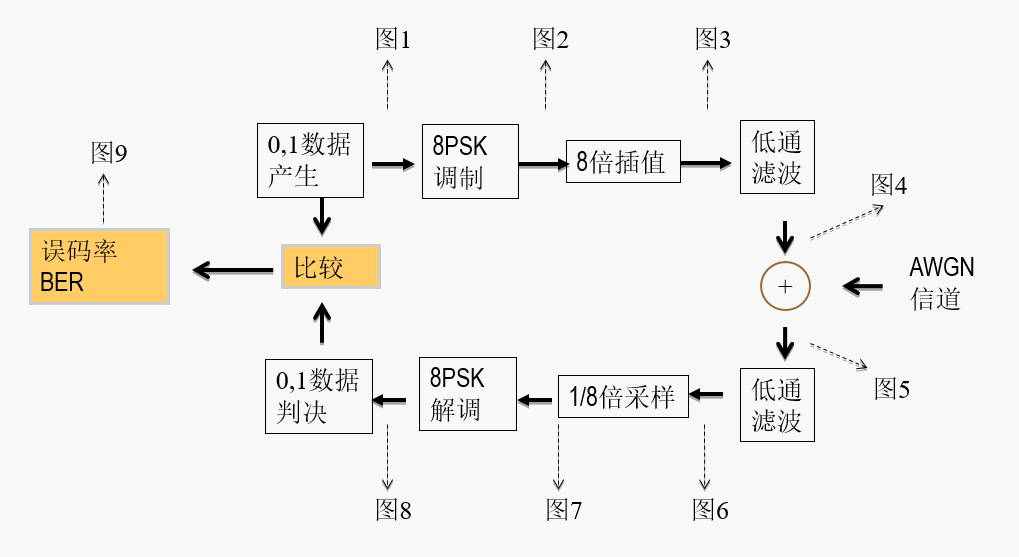
\includegraphics[width = \columnwidth]{blockdiagram.png}
\end{figure}

2. 给出原理表达式和原理框图;

3. 给出仿真程序;

4. 给出仿真结果并分析、讨论、比较;

5. 画出理论与仿真误码率曲线;

6. 将自己设计的滤波器同平方根升余弦低通滤波器比较,分析不同。


%%%%%%%%%%%%%%%%%%%%%%%%%
\section{实验原理}

\subsection{MPSK}
\begin{enumerate}

\item MPSK - multiple phase shift keying 多进制数字相位调制 , 又称多相制,是二相制的推广。它是利用载波的多种不同相位状态来表征数字信息的调制方式。多进制数字相位调制也有绝对相位调制(MPSK)和相对相位调制(MDPSK)两种。

\begin{figure}[H]
\centering
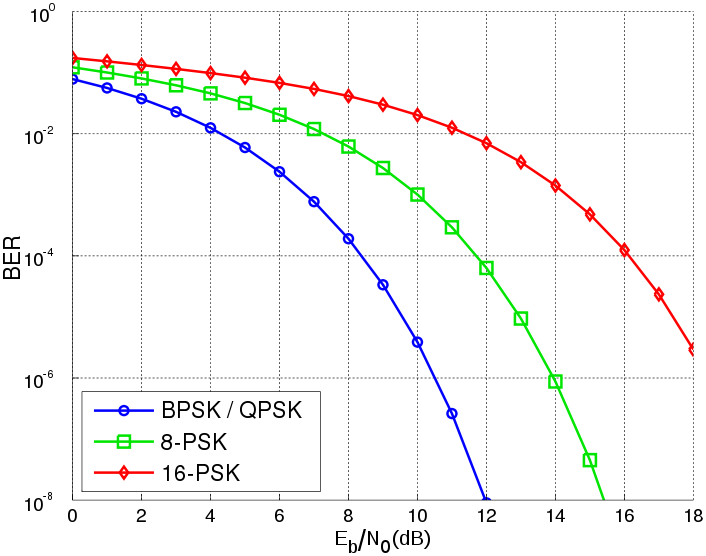
\includegraphics[width = 0.5\columnwidth]{BER.png}
\end{figure}

\item 8PSK (8 Phase Shift Keying 8移相键控) 是一种相位调制算法。相位调制(调相)是频率调制(调频)的一种演变,载波的相位被调整用于把数字信息的比特编码到每一词相位改变(相移)。因为8PSK拥有8种状态,所以8PSK每个符号(symbol)可以编码3个比特(bits)。8PSK抗链路恶化的能力(抗噪能力)不如QPSK,但提供了更高的数据吞吐容量。

\begin{figure}[H]
\centering
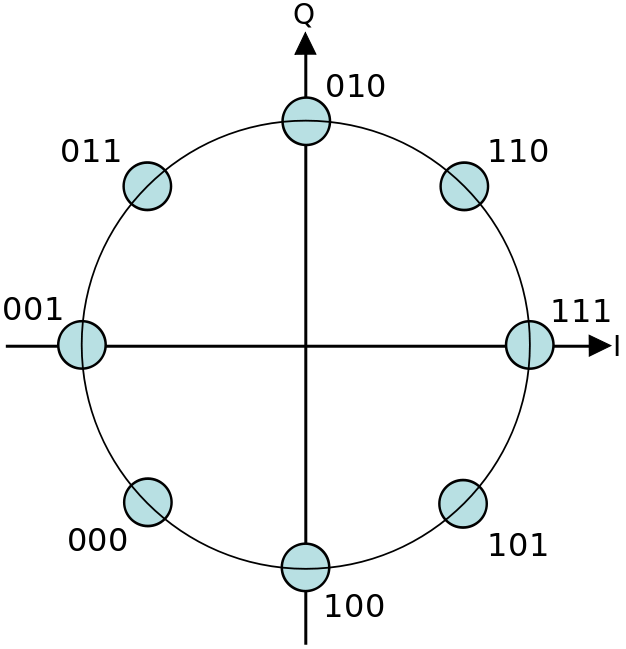
\includegraphics[width = 0.5\columnwidth]{MPSK.png}
\end{figure}


\end{enumerate}


\section{代码及仿真结果}

以自己设计的等波纹滤波器,在SNR=10处的结果为例:

\subsection{0/1数据产生}
\begin{lstlisting}
% Audio Input

clear
load /home/ykx/Audio_Communication_System/ber_standard.mat
M = 8;
K = log2(M);

% sample: datapoints of the audio
% fs: frequency of samplerate
% cnt\_point: number of datapoints
% cnt\_track: number of tunnels
basepath = '/home/ykx/Audio_Communication_System/';
wav = [basepath 'music.wav'];
[sample, fs] = audioread(wav, 'native');
info = audioinfo(wav);
[cnt_point, cnt_track] = size(sample);

% reshape to represent every symbol with 3 bits
sample = reshape(sample, [], 1);
bits = reshape(double(dectobin(sample, 16)) - 48, 3, []);
Ns = length(bits);
BER = [];   
theory = [];

% display and save
figure(1)
subplot(3,1,1)
plot(sample)
title('Audio\_TD');
subplot(3,1,2)
plot(abs(fft(sample)))
title('Audio\_FD');
subplot(3,1,3)
plot(reshape(bits, 1, []))
title('Generated Binary Sequence');
saveas(1, [basepath 'figure/audio.png']);
\end{lstlisting}

\begin{figure}[H]
\centering{}
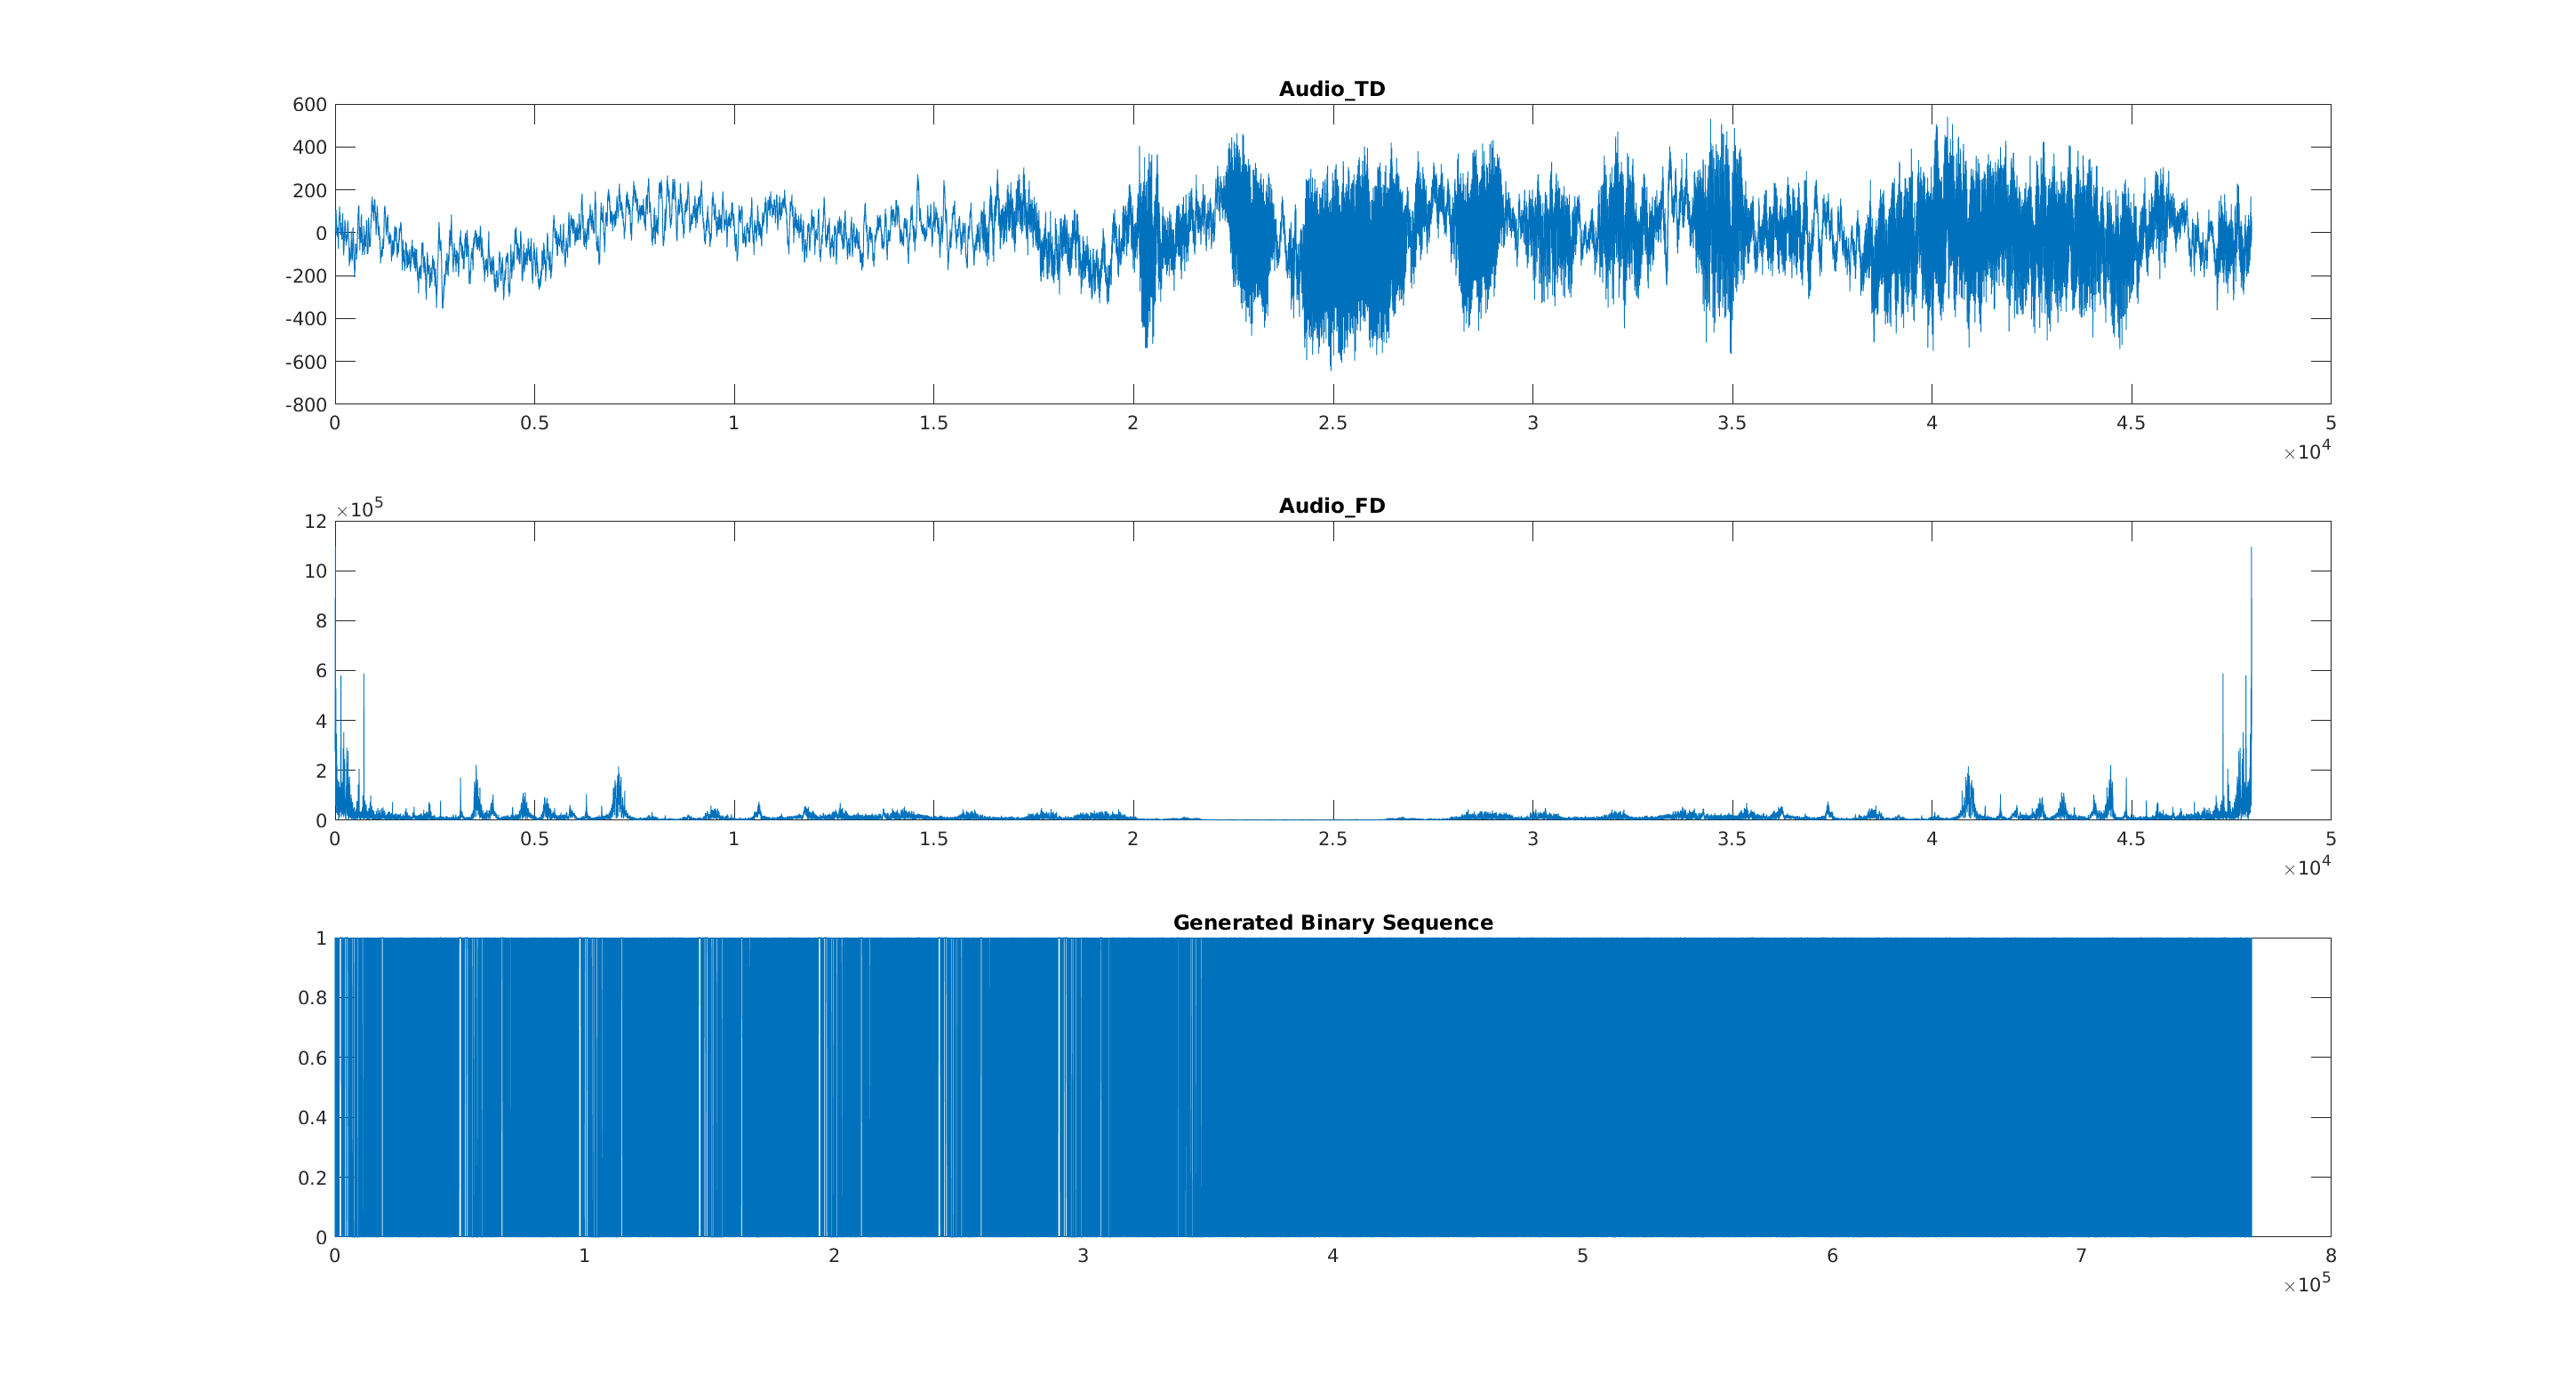
\includegraphics[width = 1\columnwidth]{audio.png}
\end{figure}

读取\verb|music.wav|文件,受计算能力的限制,音频文件选取采样率为8000Hz,量化位数为16bits,时长为6s,总点数为48000,量化后比特数为768000,以3bits一组,构成3*256000数组。

上图显示的依次是音频的时域、频域图像,以及量化成比特序列后的图像。

\subsection{8PSK调制}

\begin{lstlisting}
% Generate 8PSK Signal

%8PSK symbols
sym_map=[1;(1+1i)/sqrt(2);1i;(-1+1i)/sqrt(2);-1;(-1-1i)/sqrt(2);-1i;(1-1i)/sqrt(2)]; 

s_mpsk = [];
s_I = [];
s_Q = [];

k = 4 * bits(1, :) + 2 * bits(2, :) + bits(3, :) + 1;
s_mpsk = [s_mpsk sym_map(k)];
s_I = [s_I real(sym_map(k))]; % the I branch of 8PSK
s_Q = [s_Q imag(sym_map(k))]; % the Q branch of 8PSK
s = [s_I s_Q];

% display and save
figure(2)
subplot(2,1,1)
stem(s_I, '.')
title('Signal\_I')
subplot(2,1,2)
stem(s_Q, '.')
title('Signal\_Q')
saveas(2, [basepath 'figure/8psk.png']);
\end{lstlisting}

\begin{figure}[H]
\centering
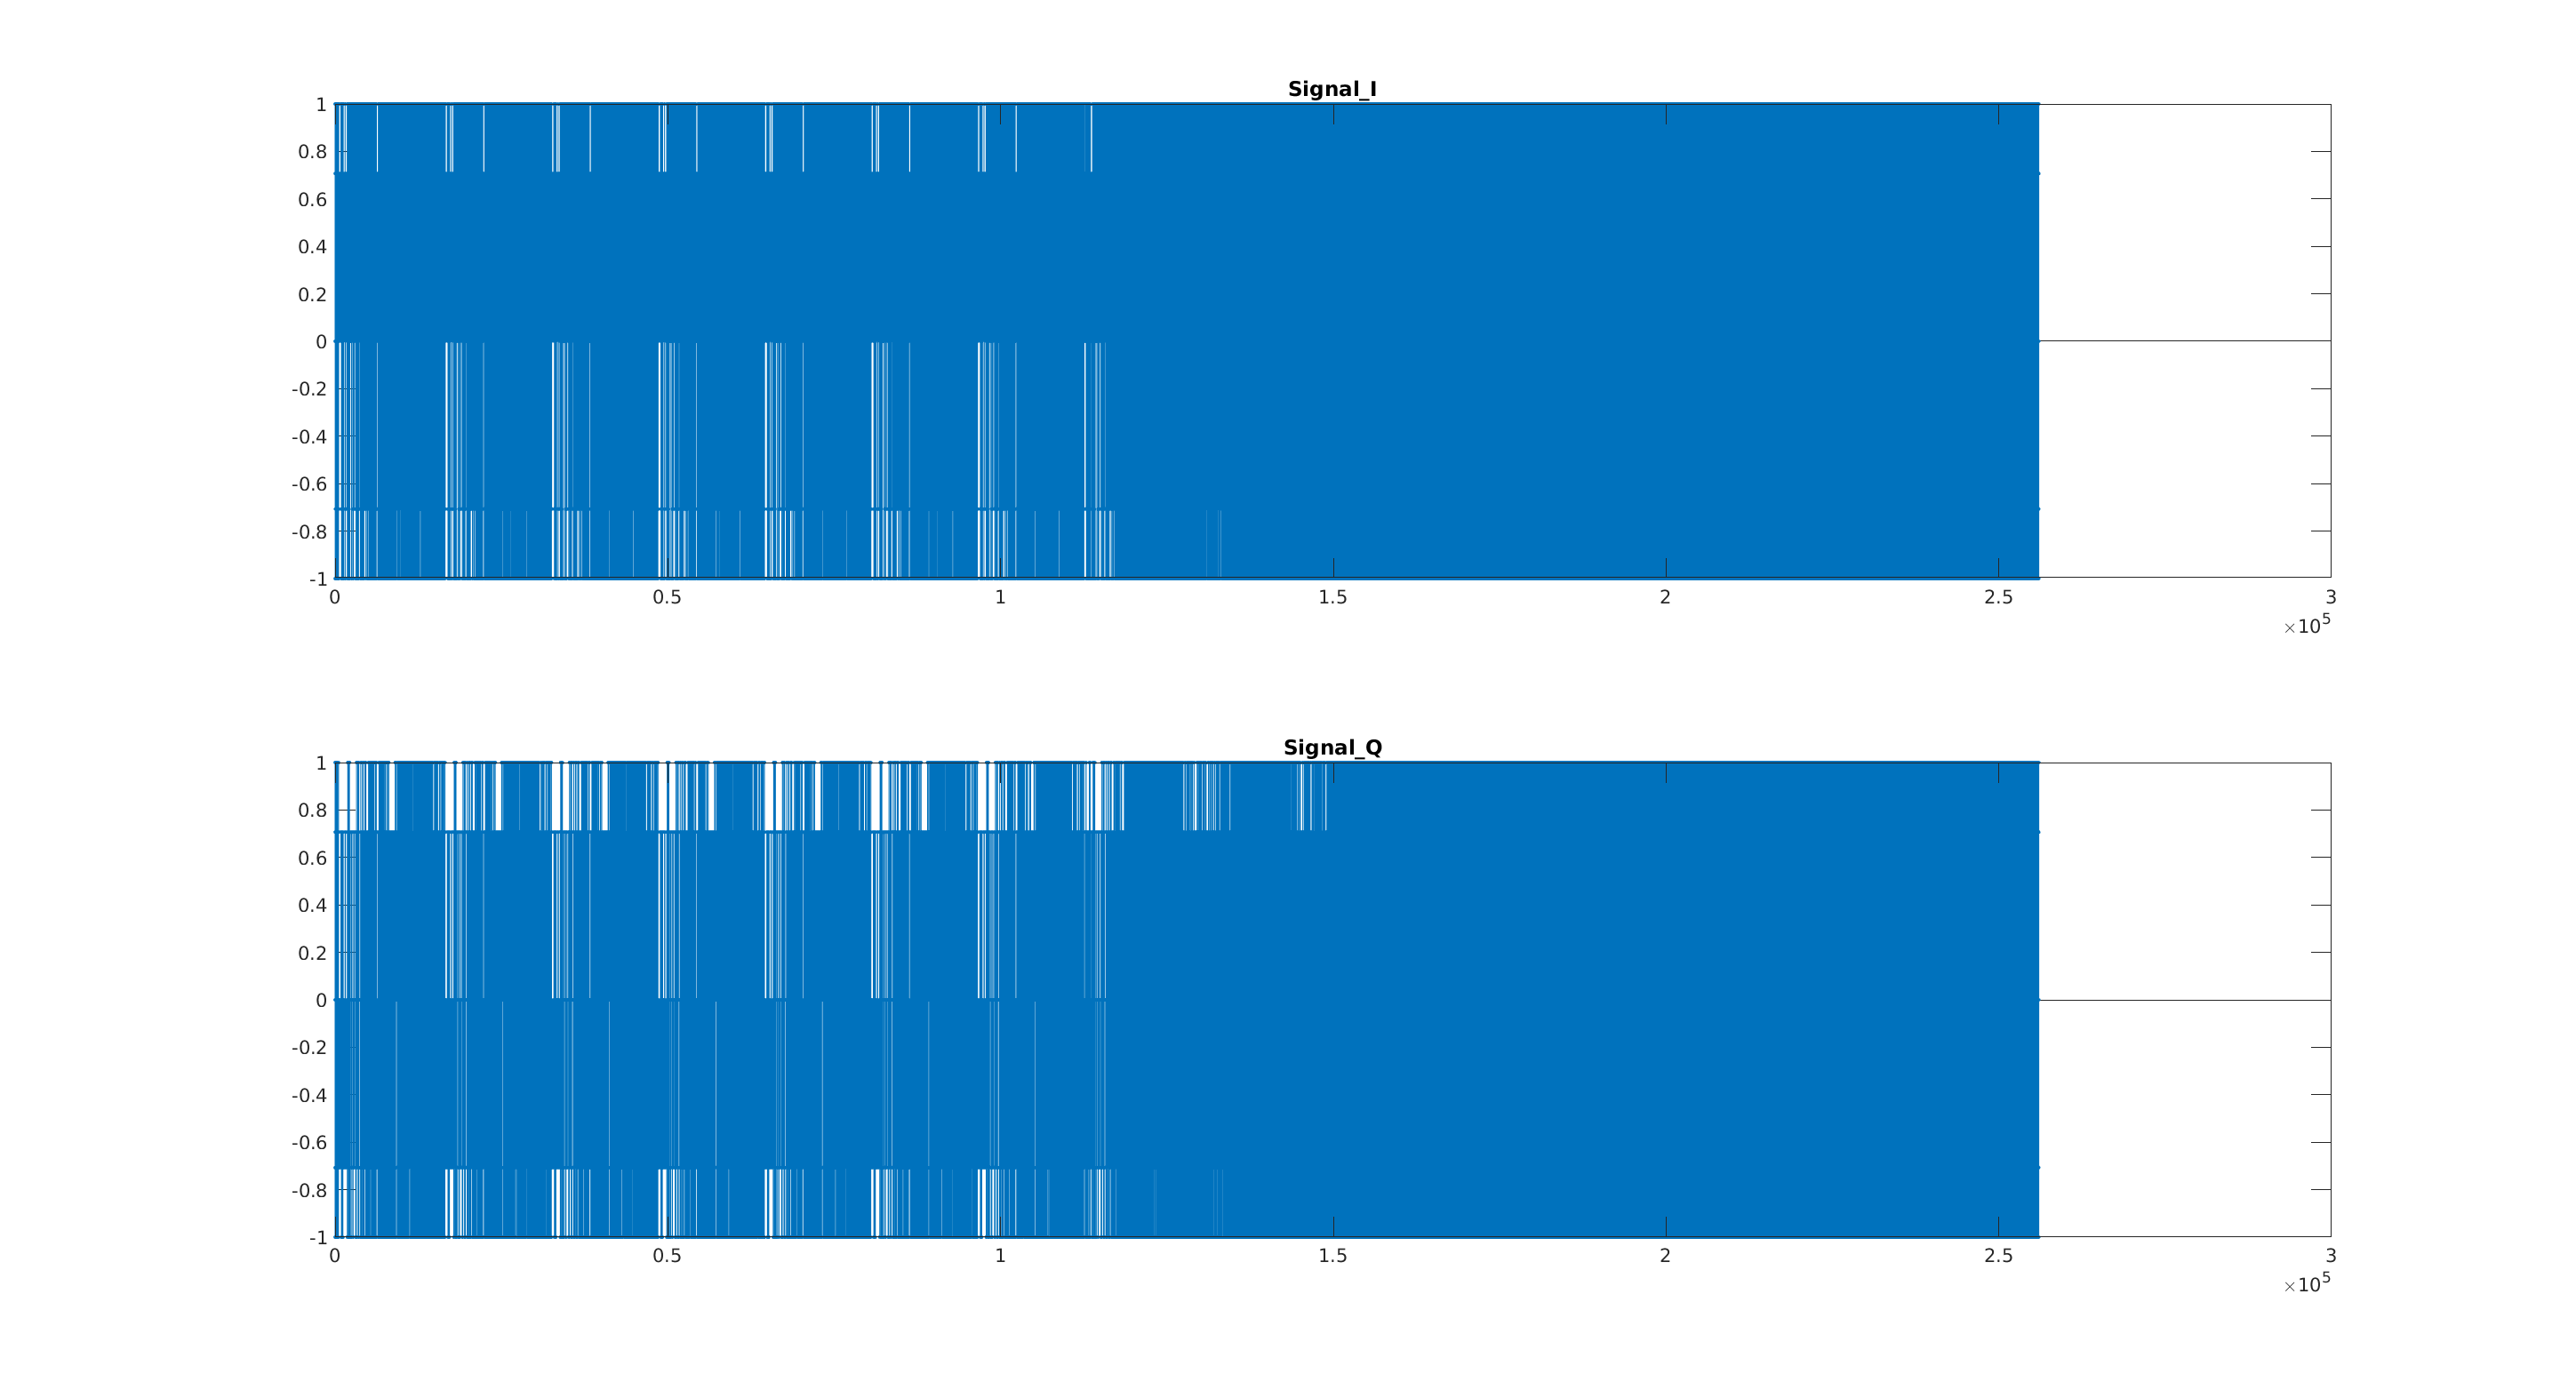
\includegraphics[width = \columnwidth]{8psk.png}
\end{figure}

3bits一组做8PSK调制,映射成复数信号s\_mpsk,分离成两路实信号s\_I,s\_Q。

上图分别显示了s\_I和s\_Q的时域波形。

\subsection{8倍插值}

\begin{lstlisting}
% Upsample

s_upsample = upsample(s, 8);

% display and save
figure(3)
subplot(4,1,1)
stem(s_upsample(:,1), '.');
title('Upsample\_I\_TD')
subplot(4,1,2)
stem(abs(fft(s_upsample(:,1))), '.');
title('Upsample\_I\_FD')
subplot(4,1,3)
stem(s_upsample(:,2), '.');
title('Upsample\_Q\_TD')
subplot(4,1,4)
stem(abs(fft(s_upsample(:,2))), '.');
title('Upsample\_Q\_FD')
saveas(3, [basepath 'figure/upsample.png']);
\end{lstlisting}

\begin{figure}[H]
\centering
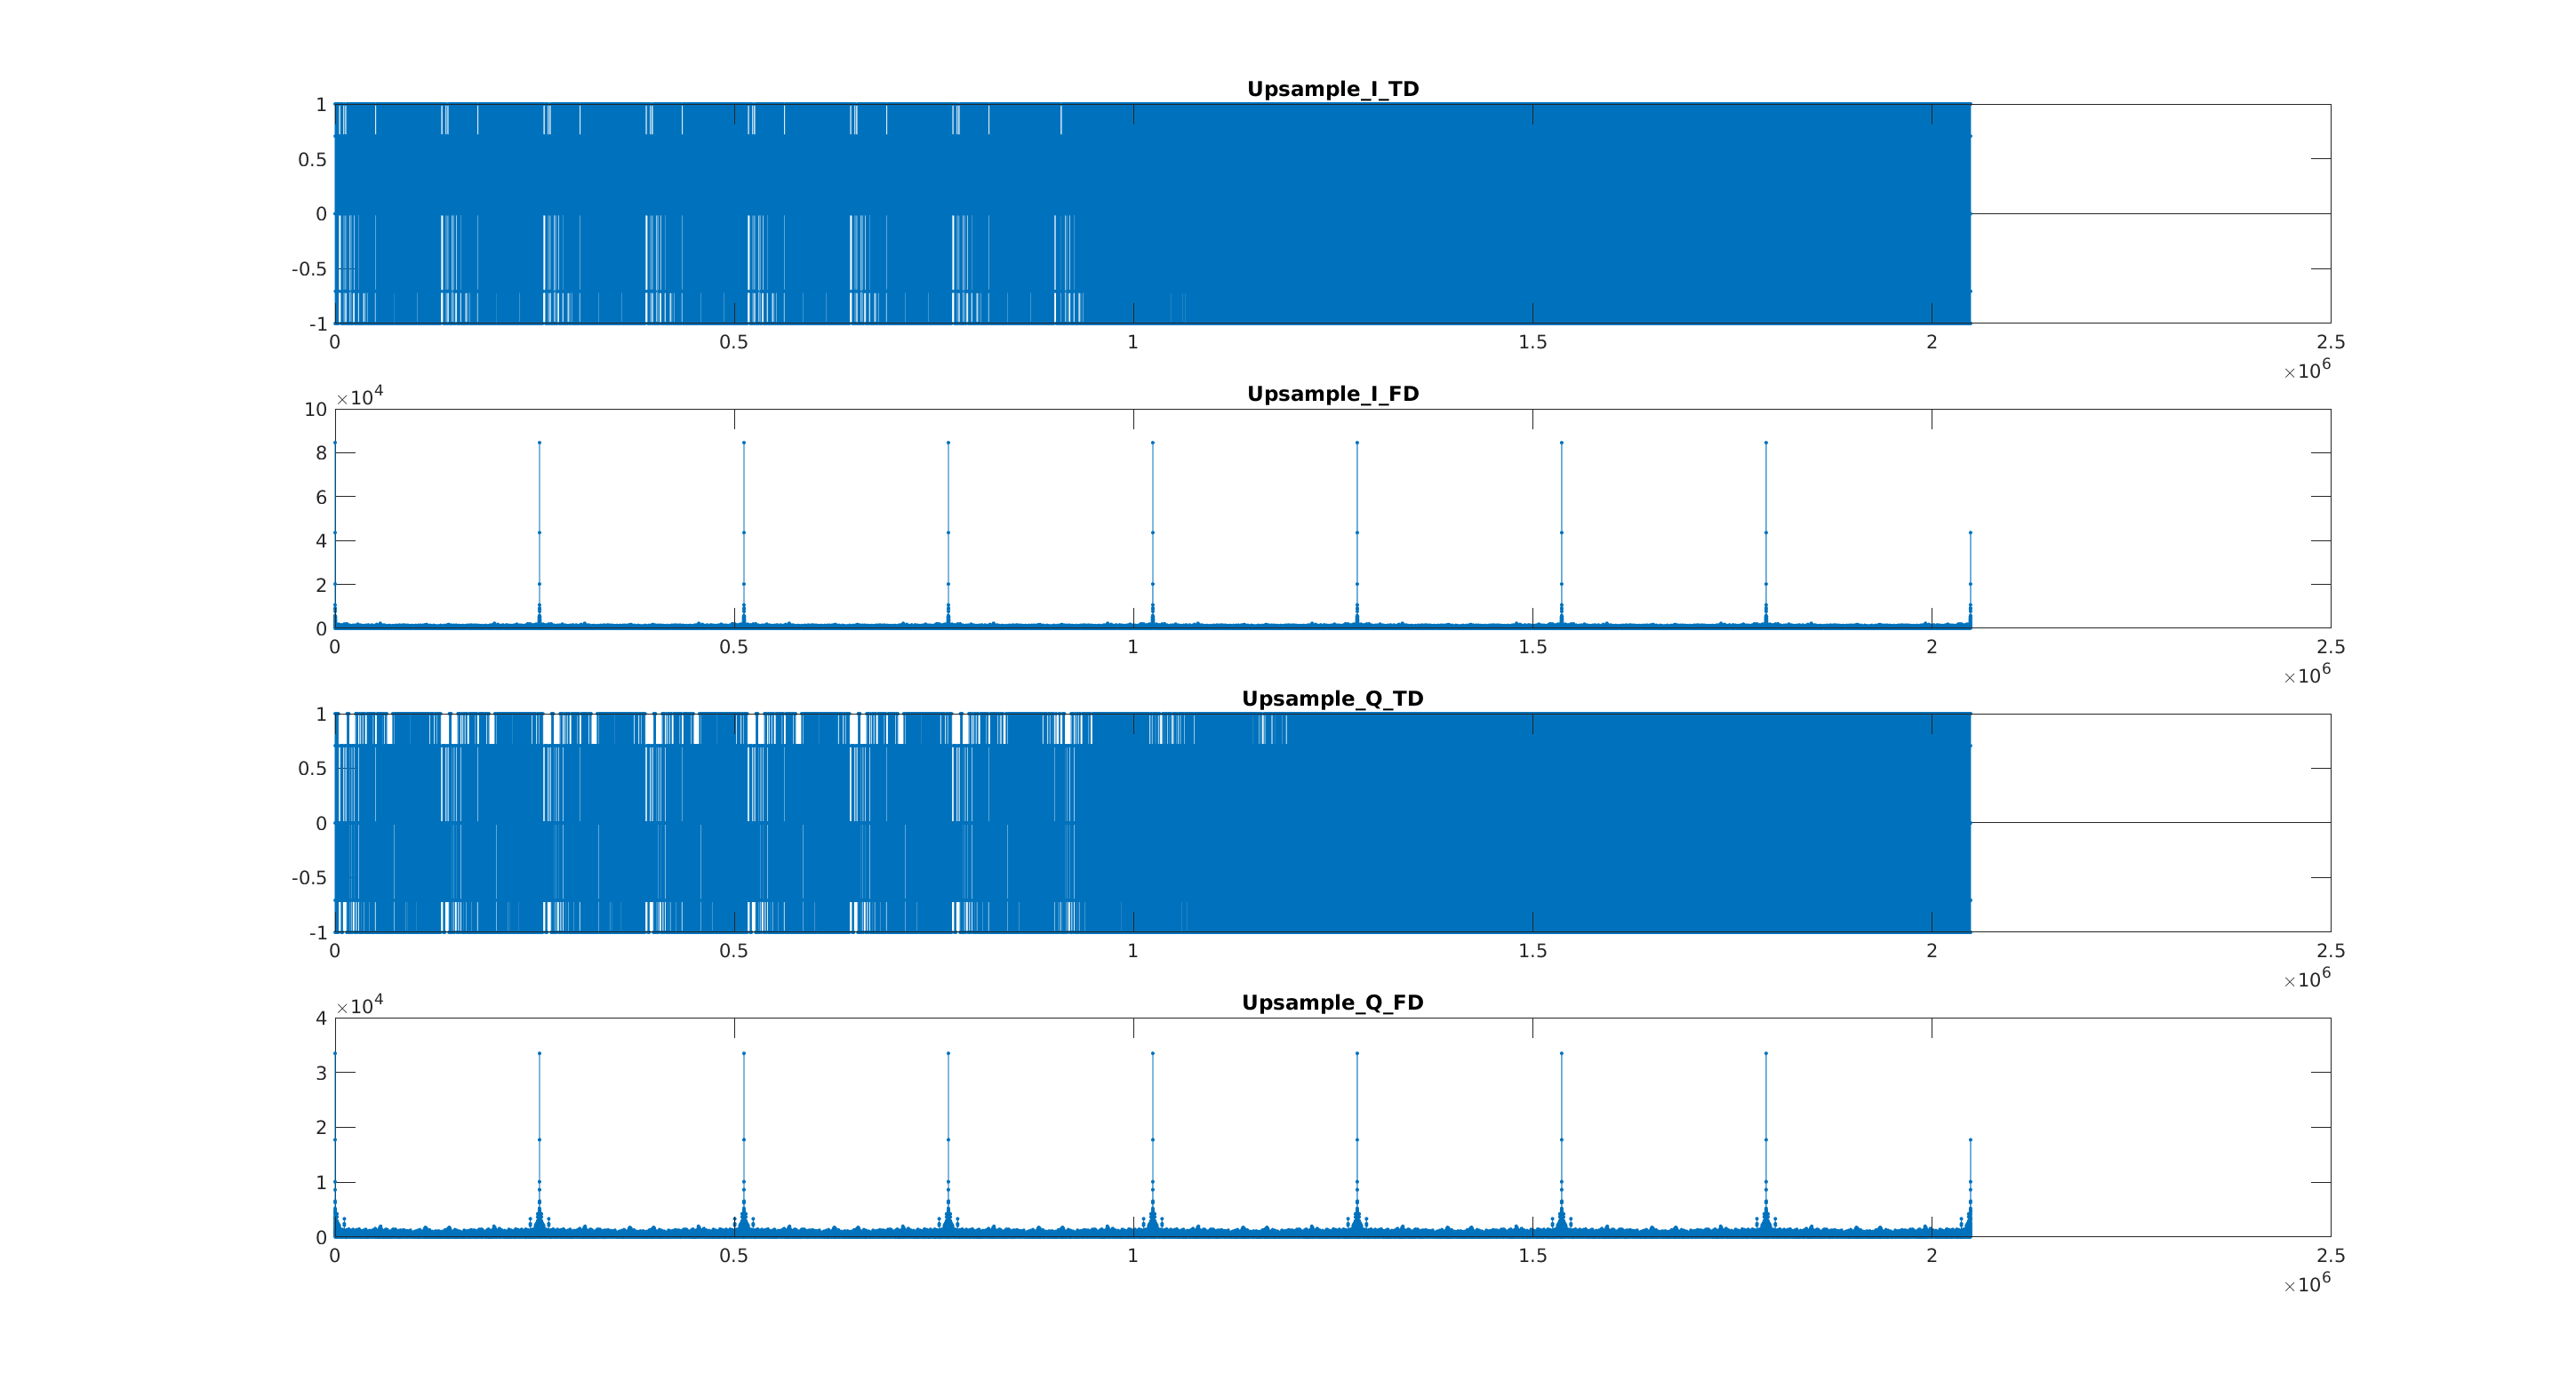
\includegraphics[width = \columnwidth]{upsample.png}
\end{figure}

分别对两支路做8倍上采样得到时域与频域波形如上,可以看到数字频域在0到$2\pi$范围内以$2\pi/8$的间隔重复8次。

\subsection{成型滤波}

首先设计了一个等波纹滤波器,参数设置上,$F_s$选取为2倍信号频率,即$2 * 128000 * 8 / 3 \approx 682666 Hz$,通带频率为$128000 / 3 \approx 42666 Hz$,阻带频率为$128000 / 3 + 4000 \approx  46666 Hz$,通带和阻带波纹分别为1dB和80dB。

\begin{figure}[H]
\centering
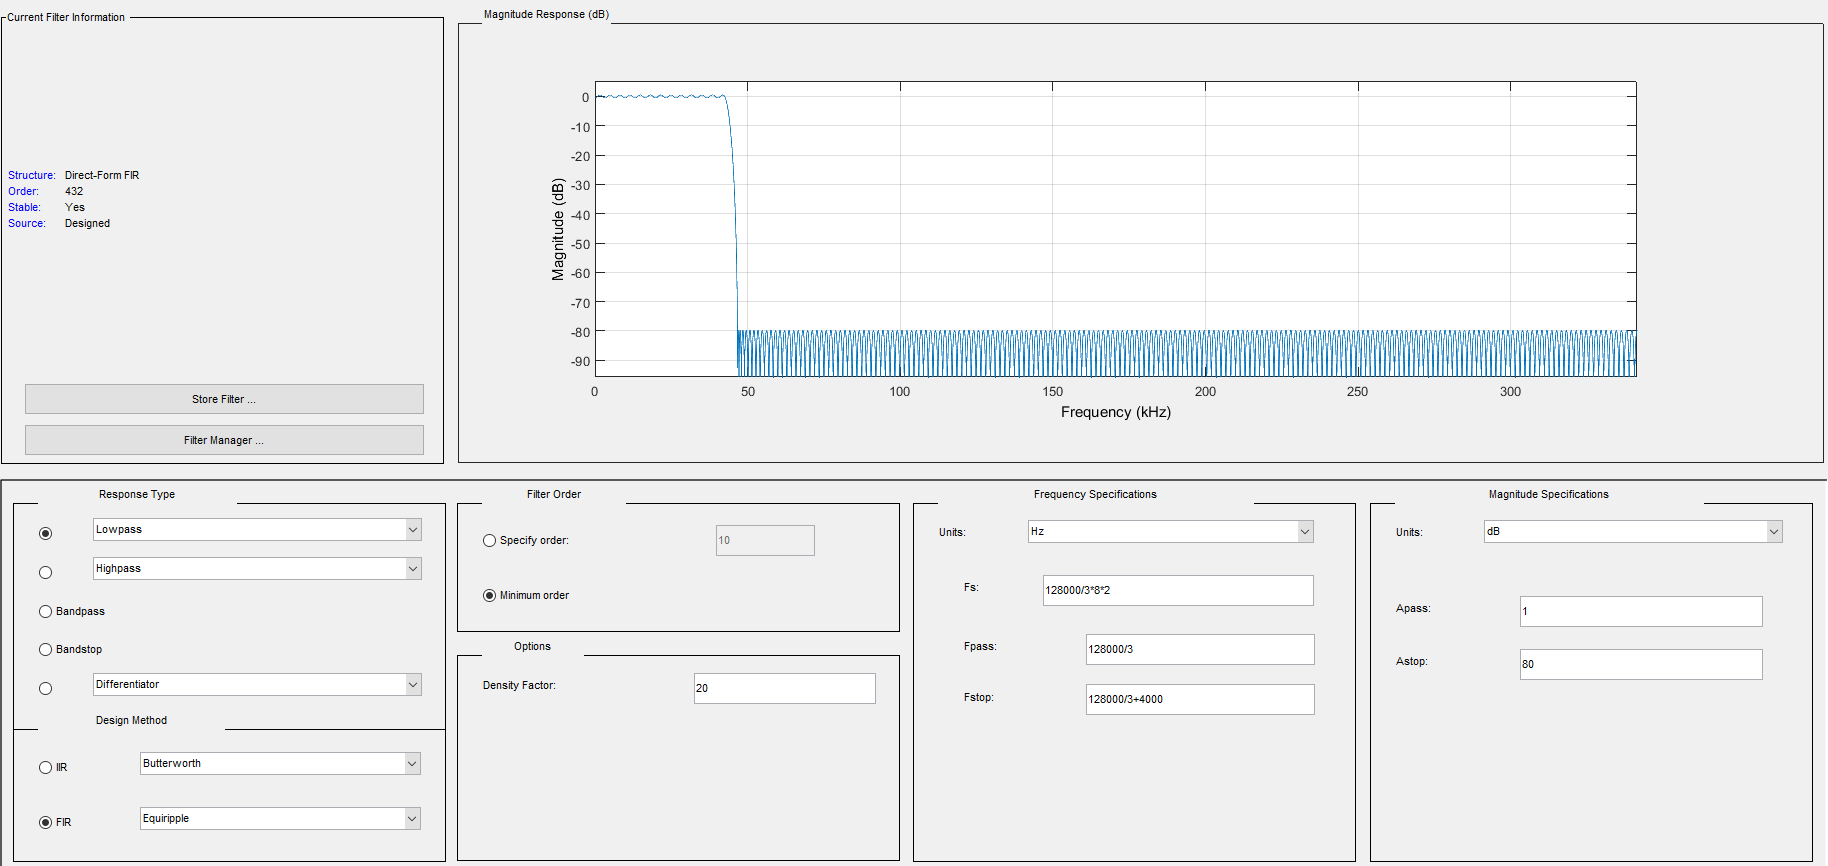
\includegraphics[width = 0.8\columnwidth]{filterparam.png}
\end{figure}

\begin{figure}[H]
\centering
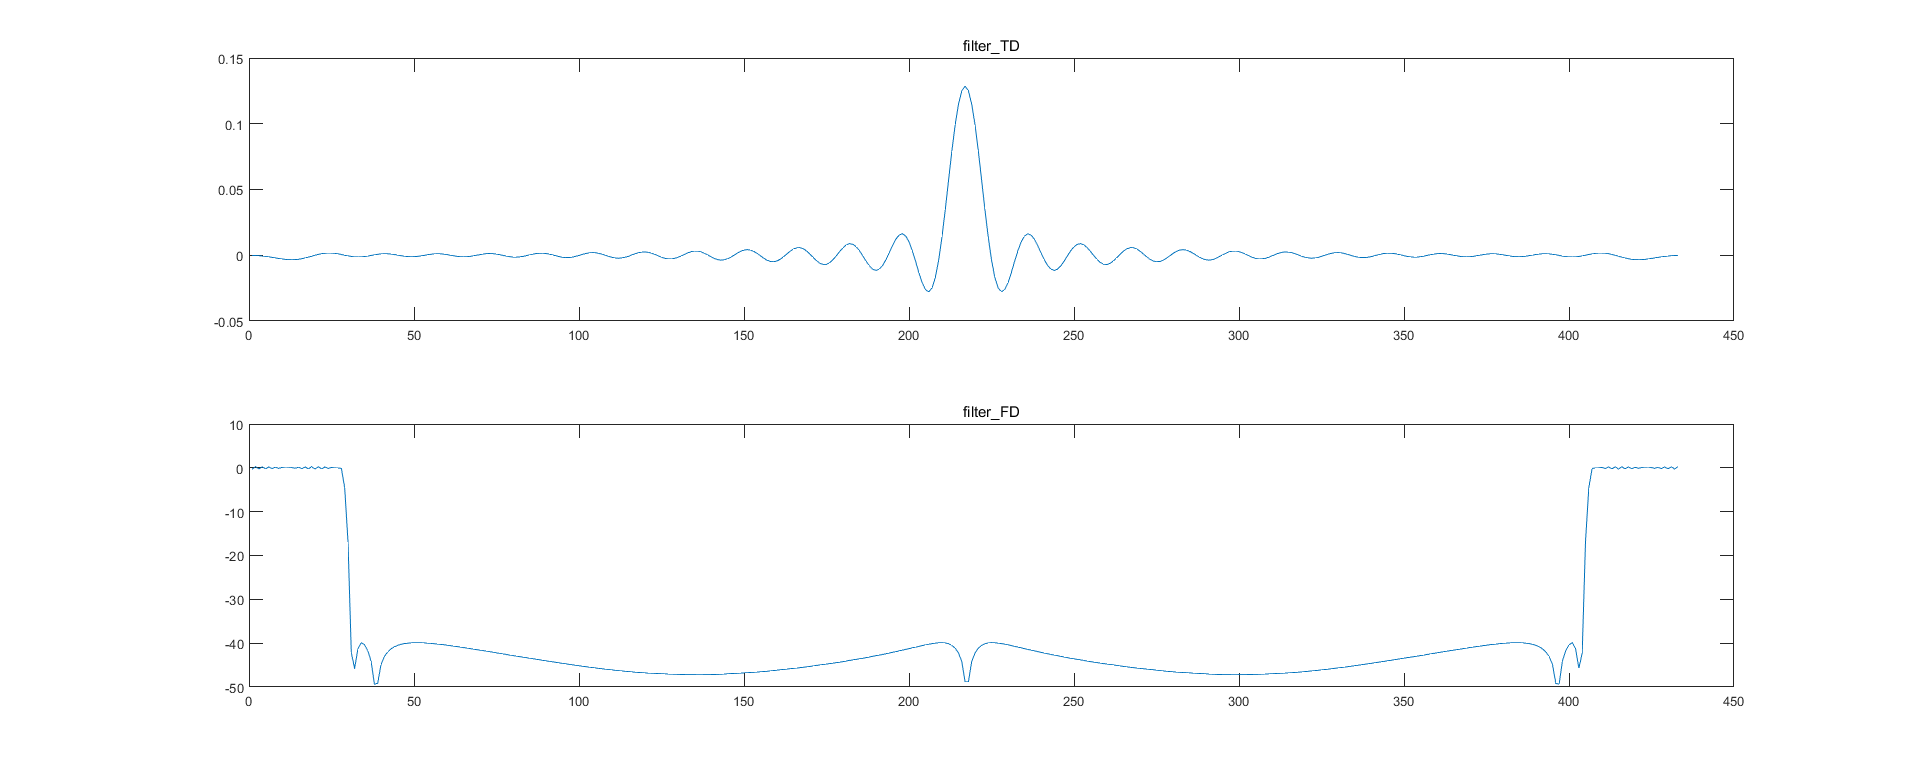
\includegraphics[width = \columnwidth]{filter.png}
\end{figure}

接下来利用该滤波器实现成型滤波:

\begin{lstlisting}
% Shaping Filter

hd = HD;
myfilter = hd.Numerator;
% add zeros after signals
s_transmit = filter(myfilter, 1, [s_upsample; zeros((length(myfilter) - 1) / 2, 2)]);
% cut off the prefix zeros
s_transmit = s_transmit(((length(myfilter)-1)/2+1): end, 1:2);

% display and save
figure(4)
subplot(2,1,1)
plot(s_transmit);
legend('signal\_I', 'signal\_Q');
title('Shaping\_TD')
subplot(2,1,2)
plot(abs(fft(s_transmit)));
legend('signal\_I', 'signal\_Q');
title('Shaping\_FD')
saveas(4, [basepath 'figure/shaping.png']);

% combine two branches
s_transmit = s_transmit(:,1) + 1i * s_transmit(:,2);
\end{lstlisting}

\begin{figure}[H]
\centering
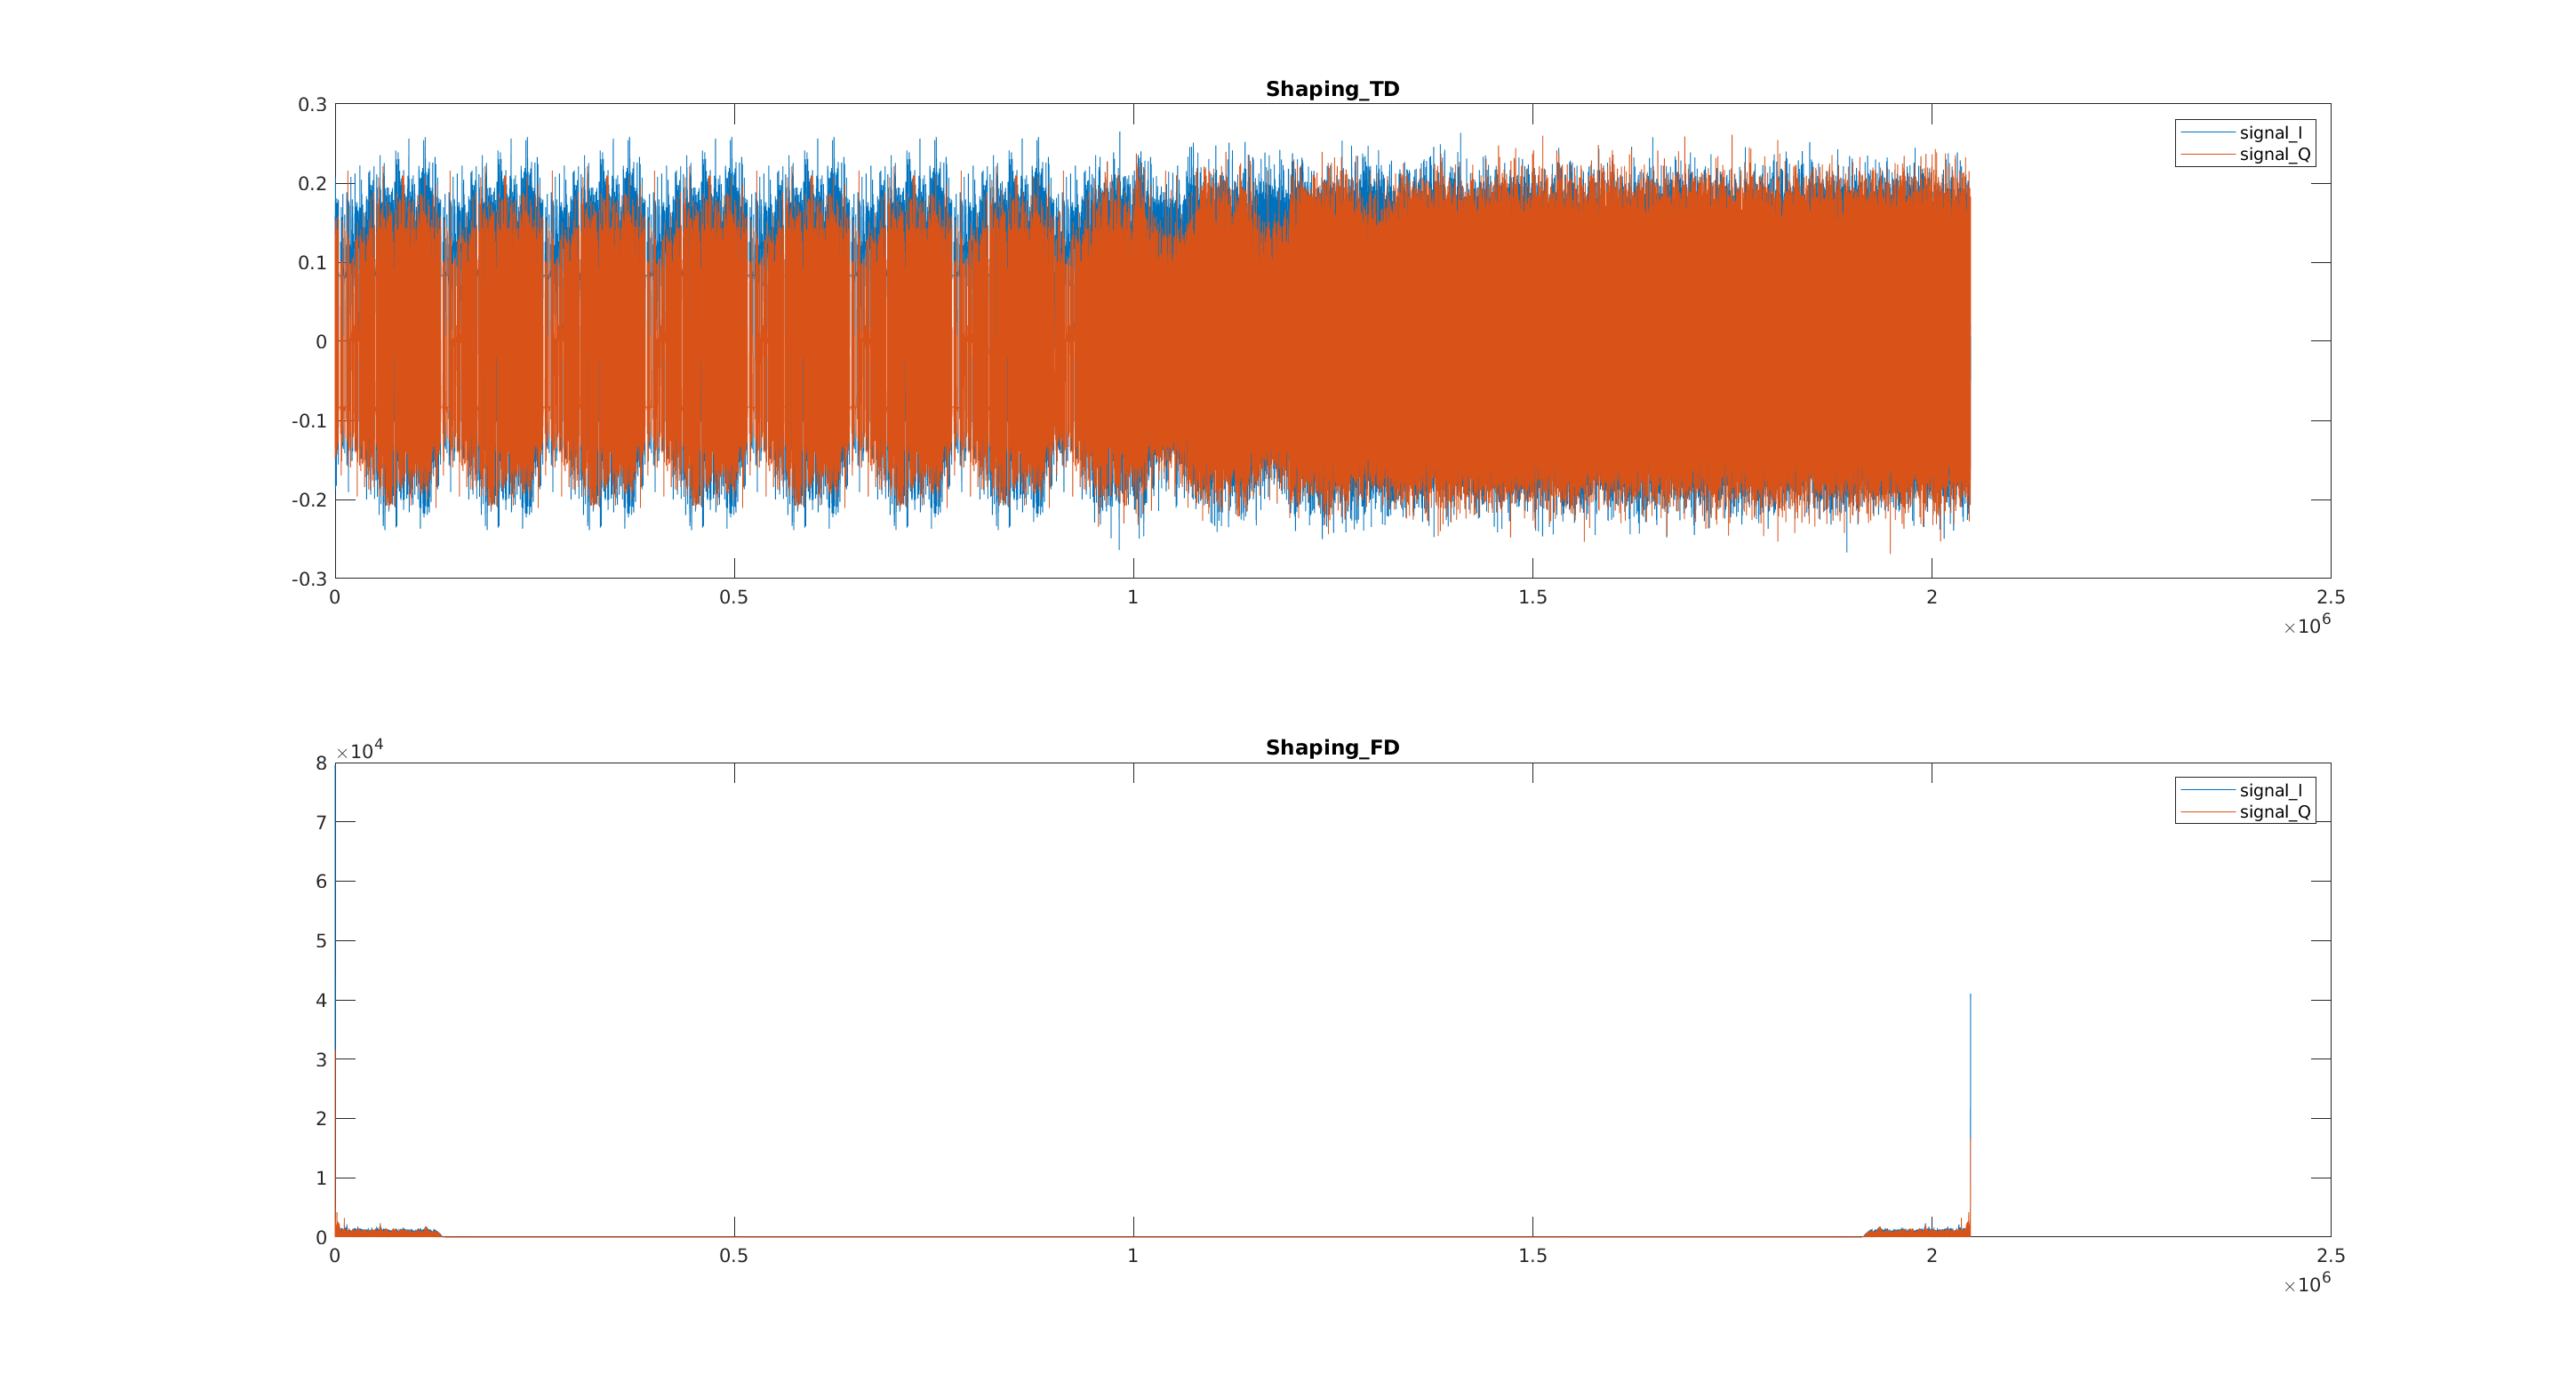
\includegraphics[width = \columnwidth]{shaping.png}
\end{figure}

由于数字滤波器存在延时效应,所以在滤波前要先在序列末尾补零,滤波后舍去序列中的前导零。

最后将两支路合并成复数信号,准备通过AWGN信道。

\subsection{AWGN信道}

\begin{lstlisting}
% AWGN Channel

Es_range = 10.^([[-7] [8:1:22]]/10); % Energy per symbol
for item = 1:16
    Es = Es_range(item);
    Eb = Es/K;                % Energy per bit
    N0 = 2;
    SNR = 10 * log10((K * Eb/N0) / 8);
    s_awgn = awgn(s_transmit, SNR, 'measured');
    
    % display and save
    figure(5)
    subplot(2,1,1)
    plot(abs(s_awgn), 'b');
    hold on;
    plot(abs(s_transmit), 'r');
    legend('after\_awgn', 'before\_awgn');
    title('AWGN\_Amplitude');
    hold off;
    subplot(2,1,2)
    plot(angle(s_awgn), 'b');
    hold on;
    plot(angle(s_transmit), 'r');
    legend('after\_awgn', 'before\_awgn');
    title('AWGN\_Angle');
    hold off;
    saveas(5, fullfile(basepath, 'figure/', string(item), '/awgn.png'));
\end{lstlisting}

\begin{figure}[H]
\centering
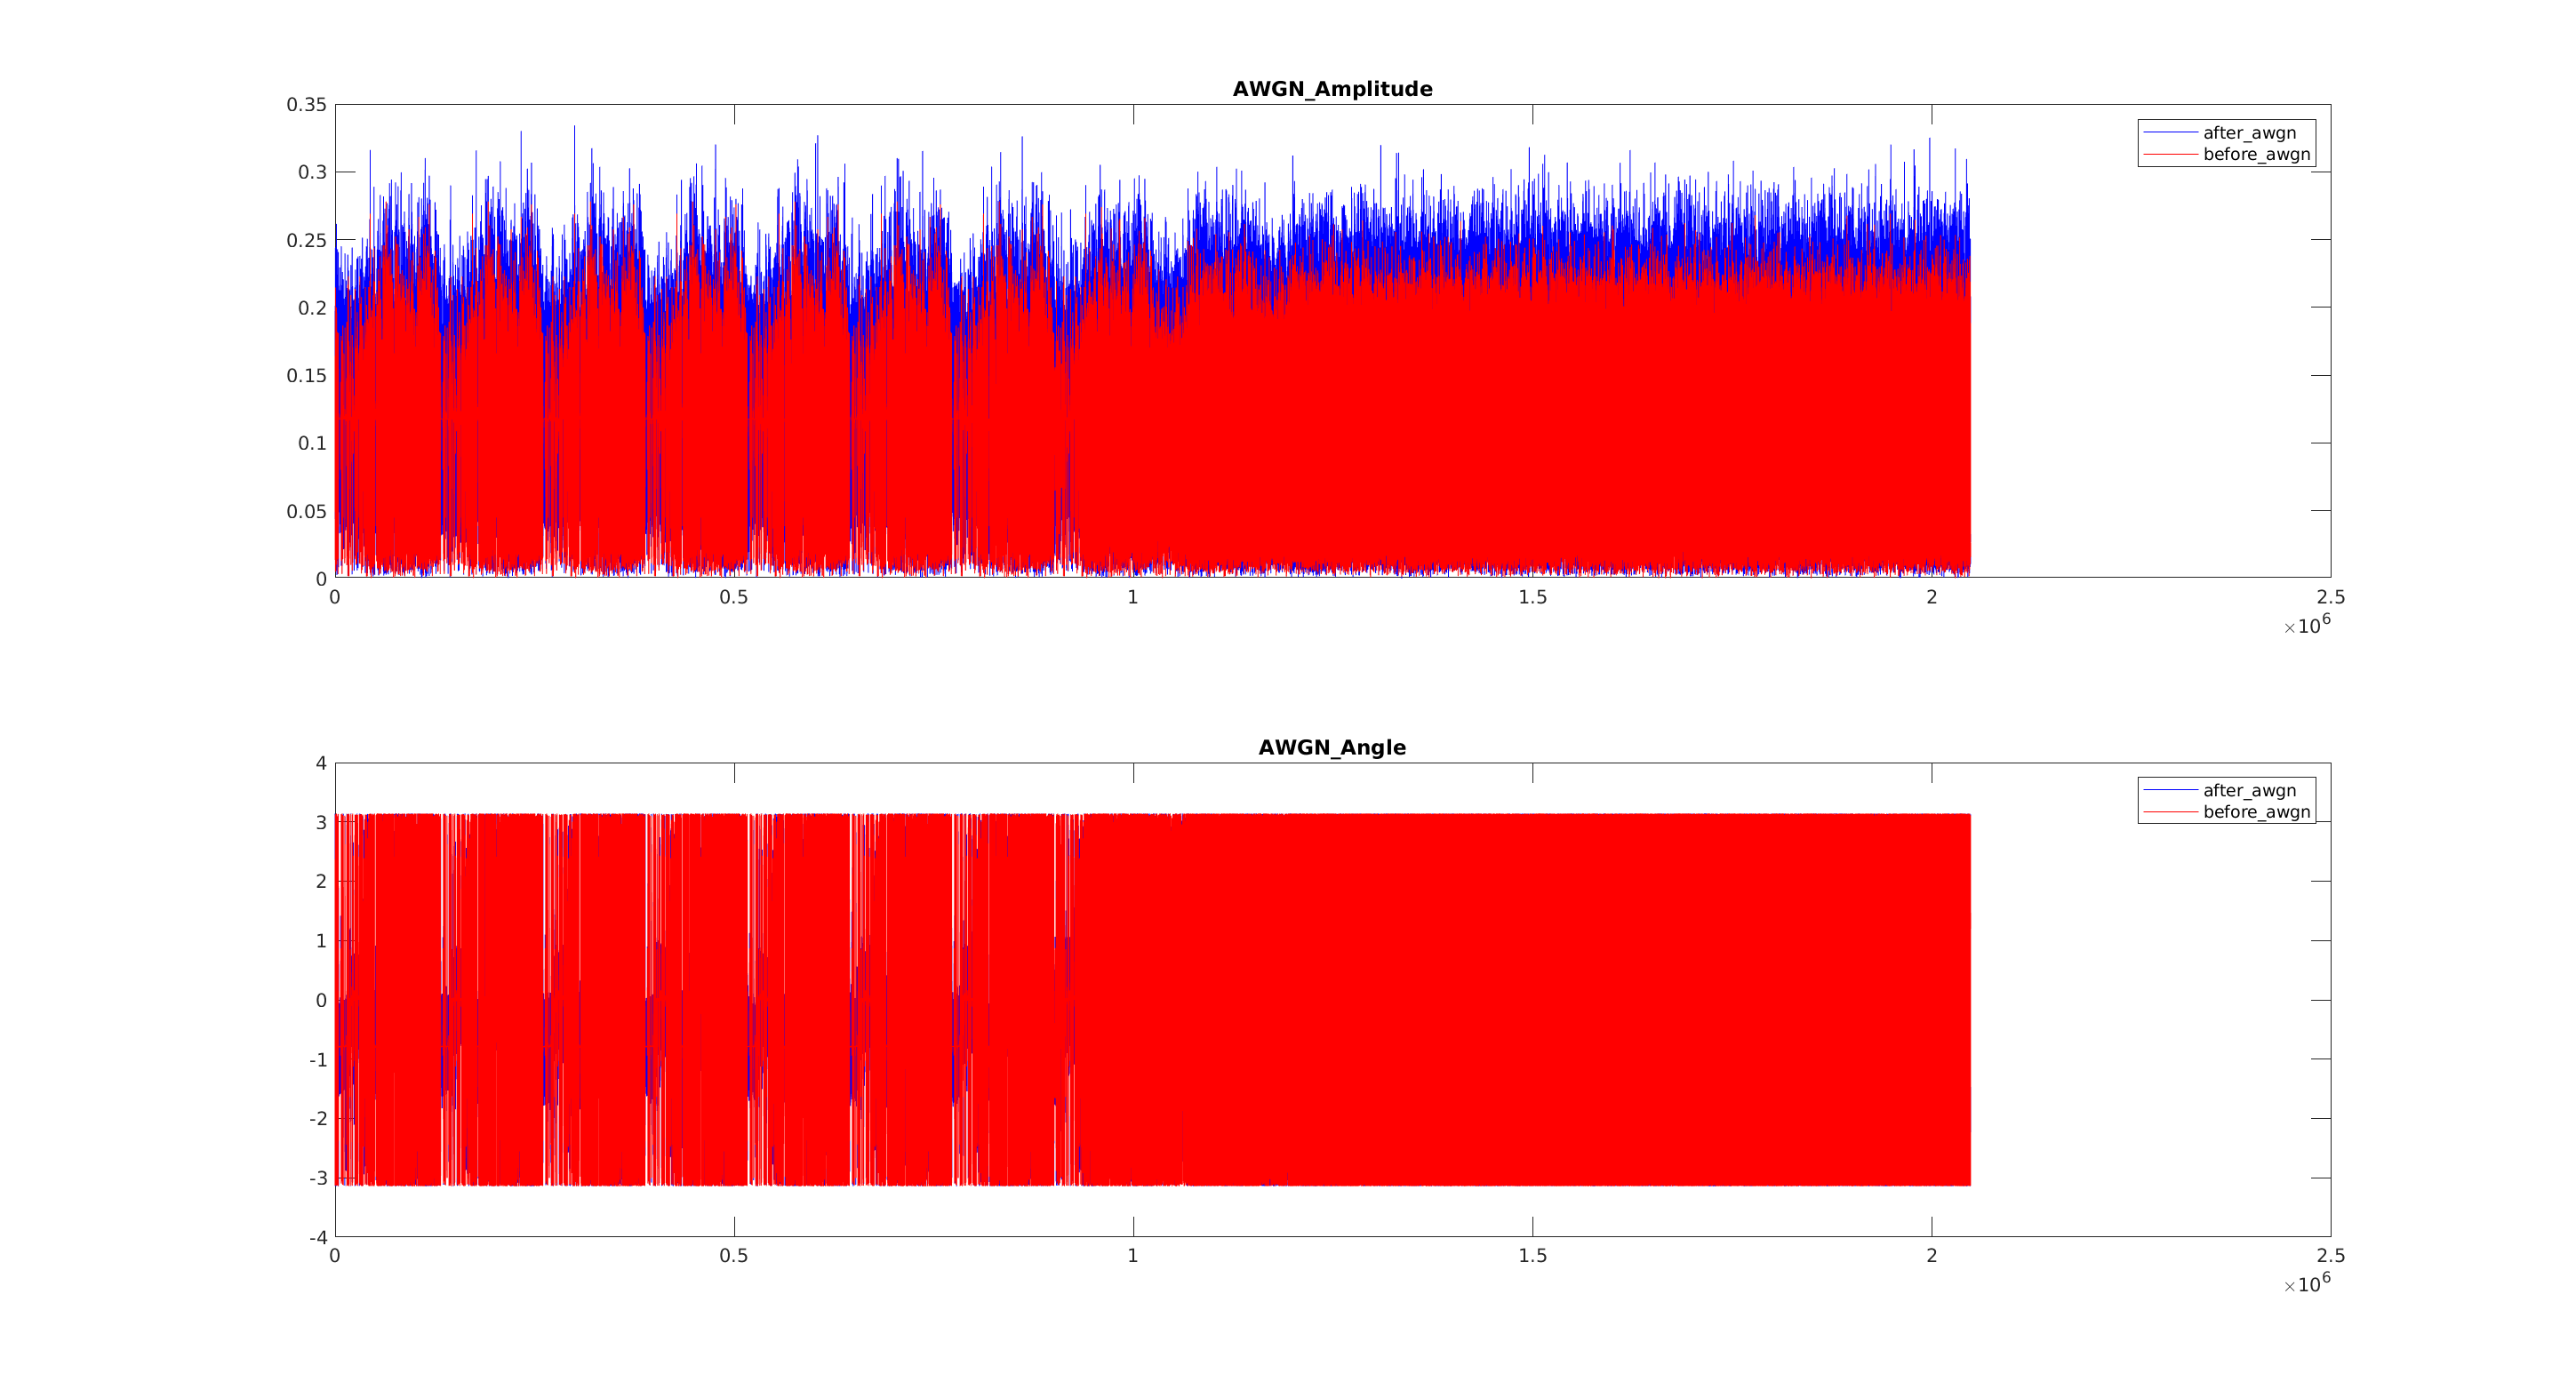
\includegraphics[width = \columnwidth]{awgn.png}
\end{figure}

设计一系列的符号功率值,循环以便最终得到BER-EbN0图像。从幅值上可以看到通过AWGN信道后,有用信号上附加了一定的噪声信号。

\subsection{低通滤波}

\begin{lstlisting}
    % Match Filter

    s_receive = filter(myfilter, 1, [s_awgn; zeros((length(myfilter) - 1) / 2, 1)]);
    s_receive = s_receive(((length(myfilter)-1)/2+1): end, 1);
    
    % display and save
    figure(6)
    subplot(3,1,1)
    plot(abs(s_receive), 'b');
    title('after filter');
    subplot(3,1,2)
    plot(abs(s_awgn), 'r');
    title('after awgn');
    subplot(3,1,3)
    plot(abs(s_transmit), 'y');
    title('before awgn');
    saveas(6, fullfile(basepath, 'figure/', string(item), '/matchedfilter.png'));
\end{lstlisting}

\begin{figure}[H]
\centering
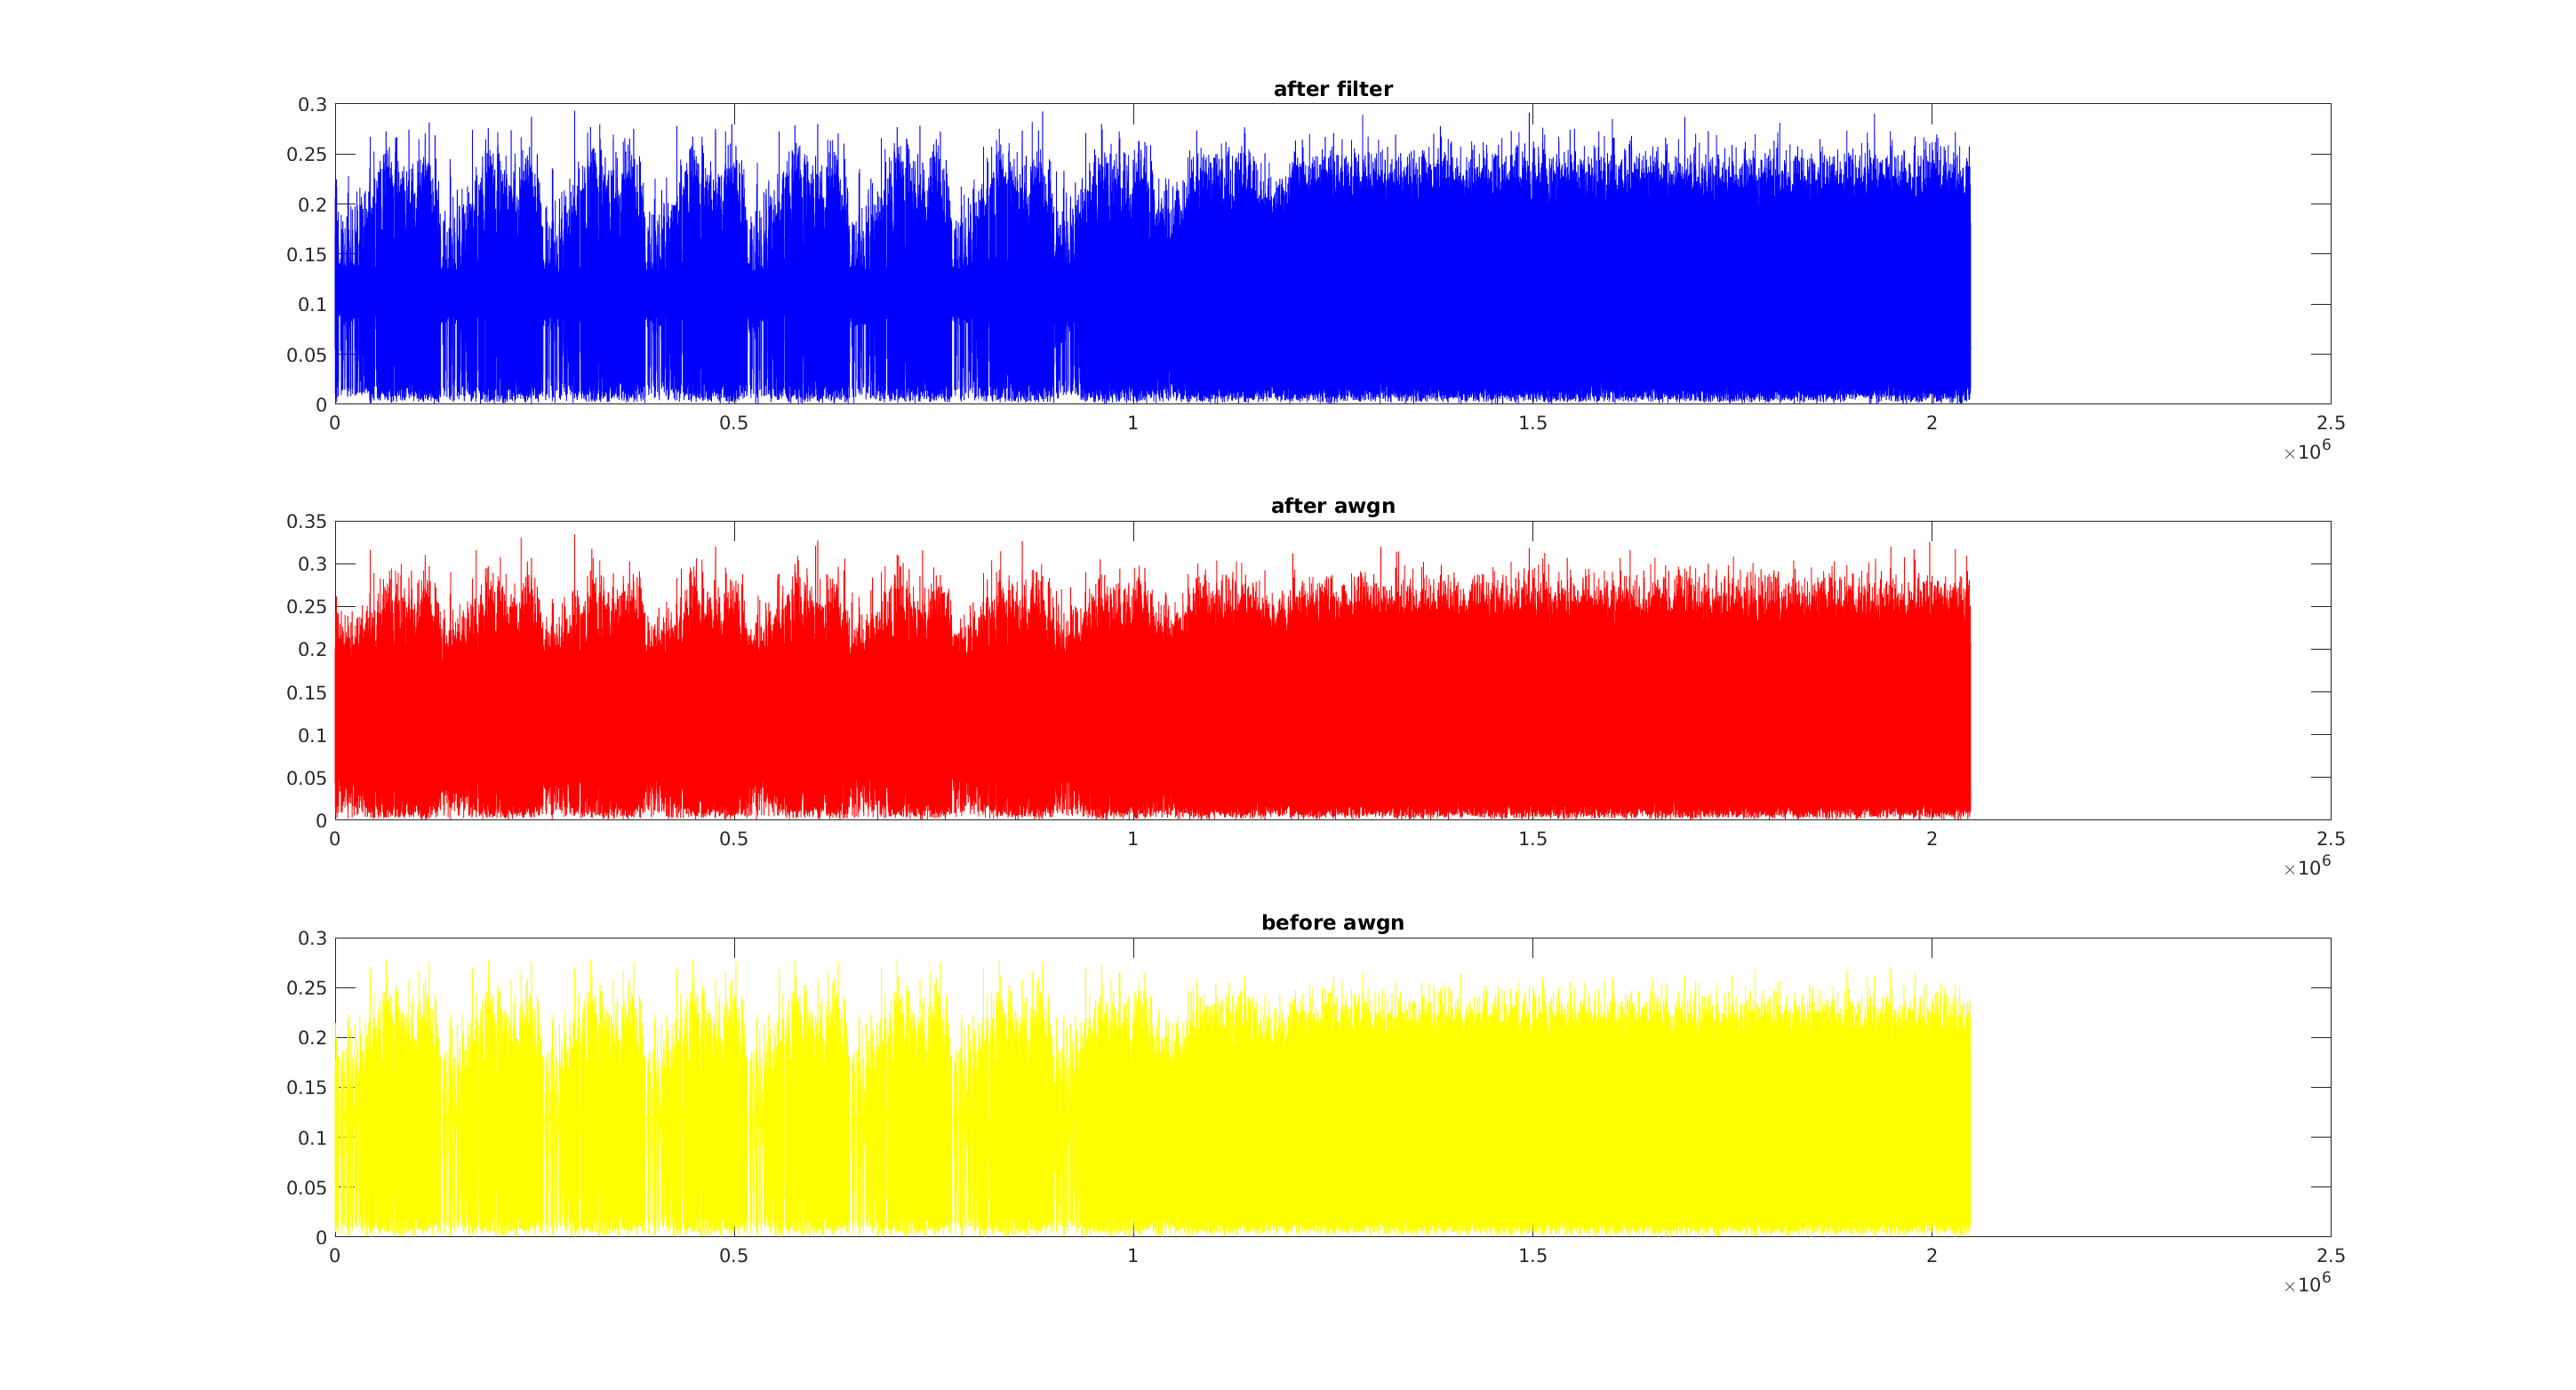
\includegraphics[width = \columnwidth]{matchedfilter.png}
\end{figure}

做一次低通滤波,由三条时域图像可以粗略看到,低通滤波后的波形更接近通过AWGN信道前的波形,部分噪声被滤除。

\subsection{1/8下采样}

\begin{lstlisting}
    % Downsample

    s_downsample = downsample(s_receive, 8);
    % divide into two branches
    s_downsample = [real(s_downsample) imag(s_downsample)];
    
    %display and save
    figure(7)
    periodogram(s_downsample);
    title('Downsample\_pdf');
    saveas(7, fullfile(basepath, 'figure/', string(item), '/downsample.png'));
\end{lstlisting}

\begin{figure}[H]
\centering
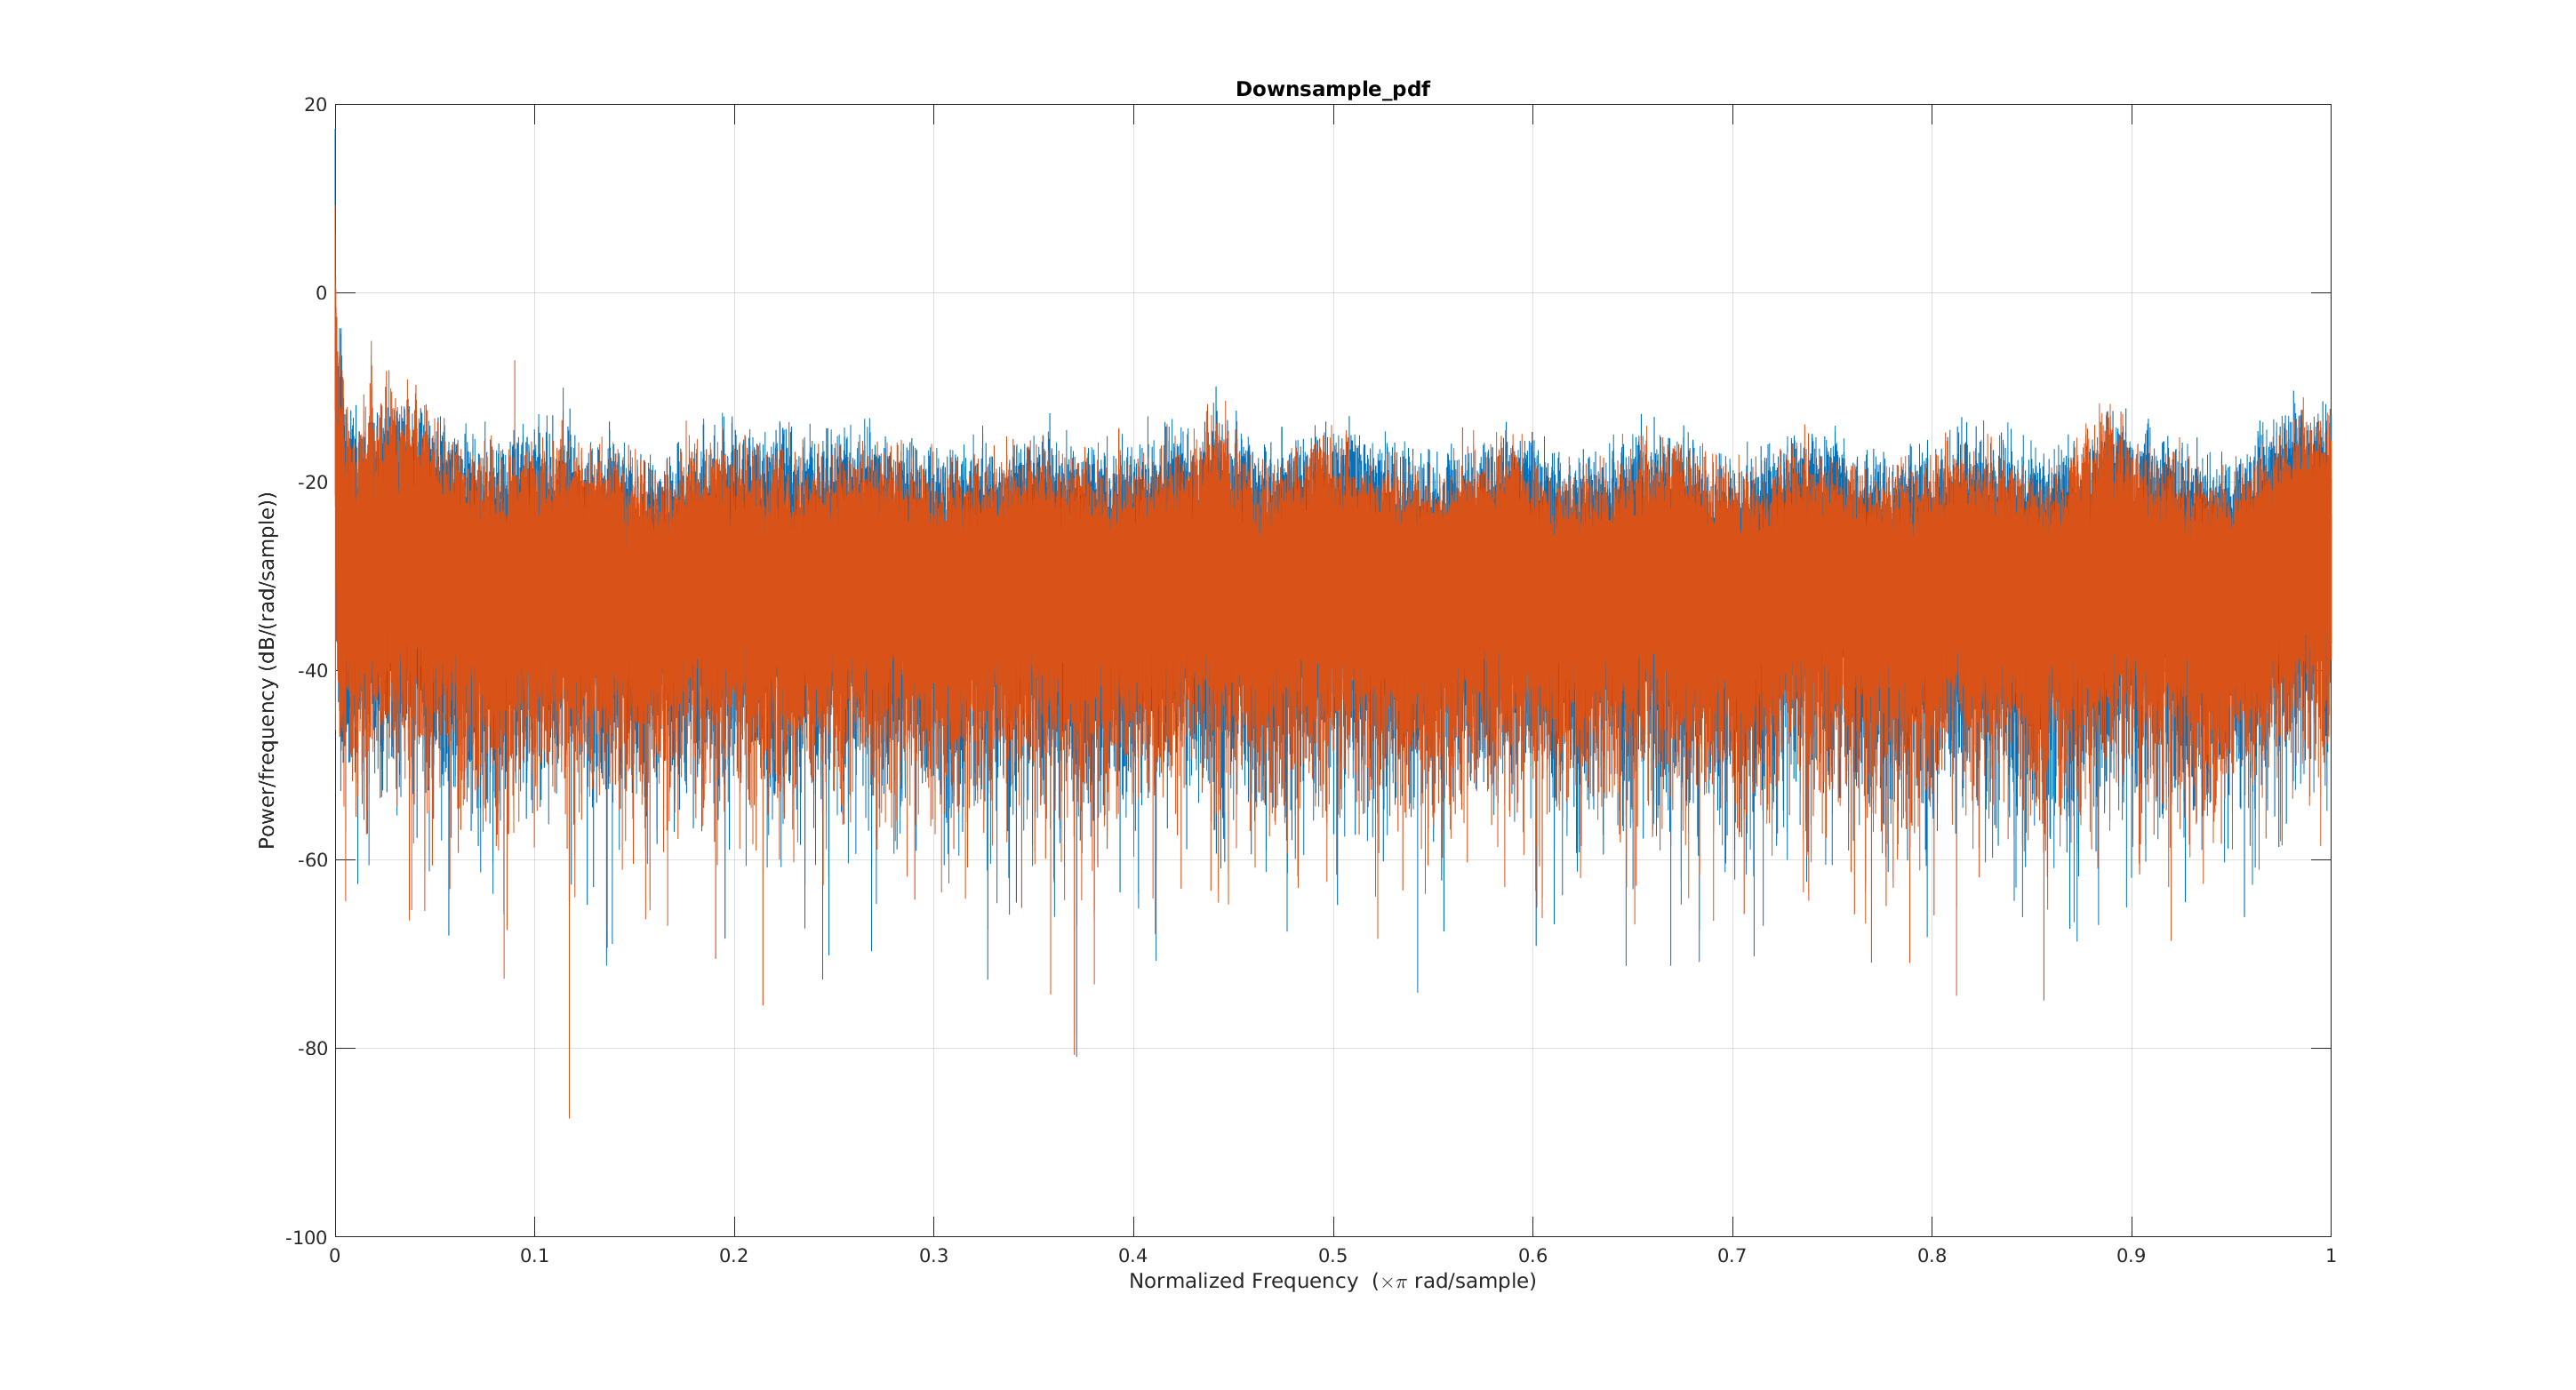
\includegraphics[width = \columnwidth]{downsample.png}
\end{figure}

做1/8下采样,并将复数信号按照实部和虚部分离成两支路,上图为两支路的功率谱密度函数图像。

\subsection{8PSK解调及判决}

\begin{lstlisting}
    % 8PSK Judgement

    s_demodulate = s_downsample;

    % display and save
    figure(8)
    plot(s_demodulate(:,1), s_demodulate(:,2), 'b.')
    title('Constellation Diagram');
    saveas(8, fullfile(basepath, 'figure/', string(item), '/constellation.png'));

    % calculate the distance to 8 phase points
    s_result = s_demodulate(:,1) - 1i * s_demodulate(:,2);
    s_result = s_result';
    distance = abs(repmat(s_result, [M, 1]) - repmat(sym_map, [1, Ns]));

    % get the minimun distance and the order
    [min_dis, min_pos] = min(uint32(distance .* 10000));

    % display and save
    figure(9)
    subplot(3,1,1)
    plot(k)
    subplot(3,1,2)
    plot(min_pos)
    subplot(3,1,3)
    plot(k-min_pos)
    saveas(9, fullfile(basepath, 'figure/', string(item), '/error.png'));

    % demodulate from symbols to bits sequence
    min_pos = min_pos - 1;
    bits_result = [];
    bits_result = [bits_result sign(bitand(min_pos, 4))]    ;
    bits_result = [bits_result; sign(bitand(min_pos, 2))];
    bits_result = [bits_result; mod(min_pos, 2)];

    % display and save
    figure(11)
    subplot(2,1,1)
    plot(reshape(bits, 1, []), 'b');
    title('transmitted\_bits');
    subplot(2,1,2)
    plot(reshape(bits_result, 1, []), 'r');
    title('received\_bits');
    saveas(11, fullfile(basepath, 'figure/', string(item), '/bits.png'));
\end{lstlisting}

\begin{figure}[H]
\centering
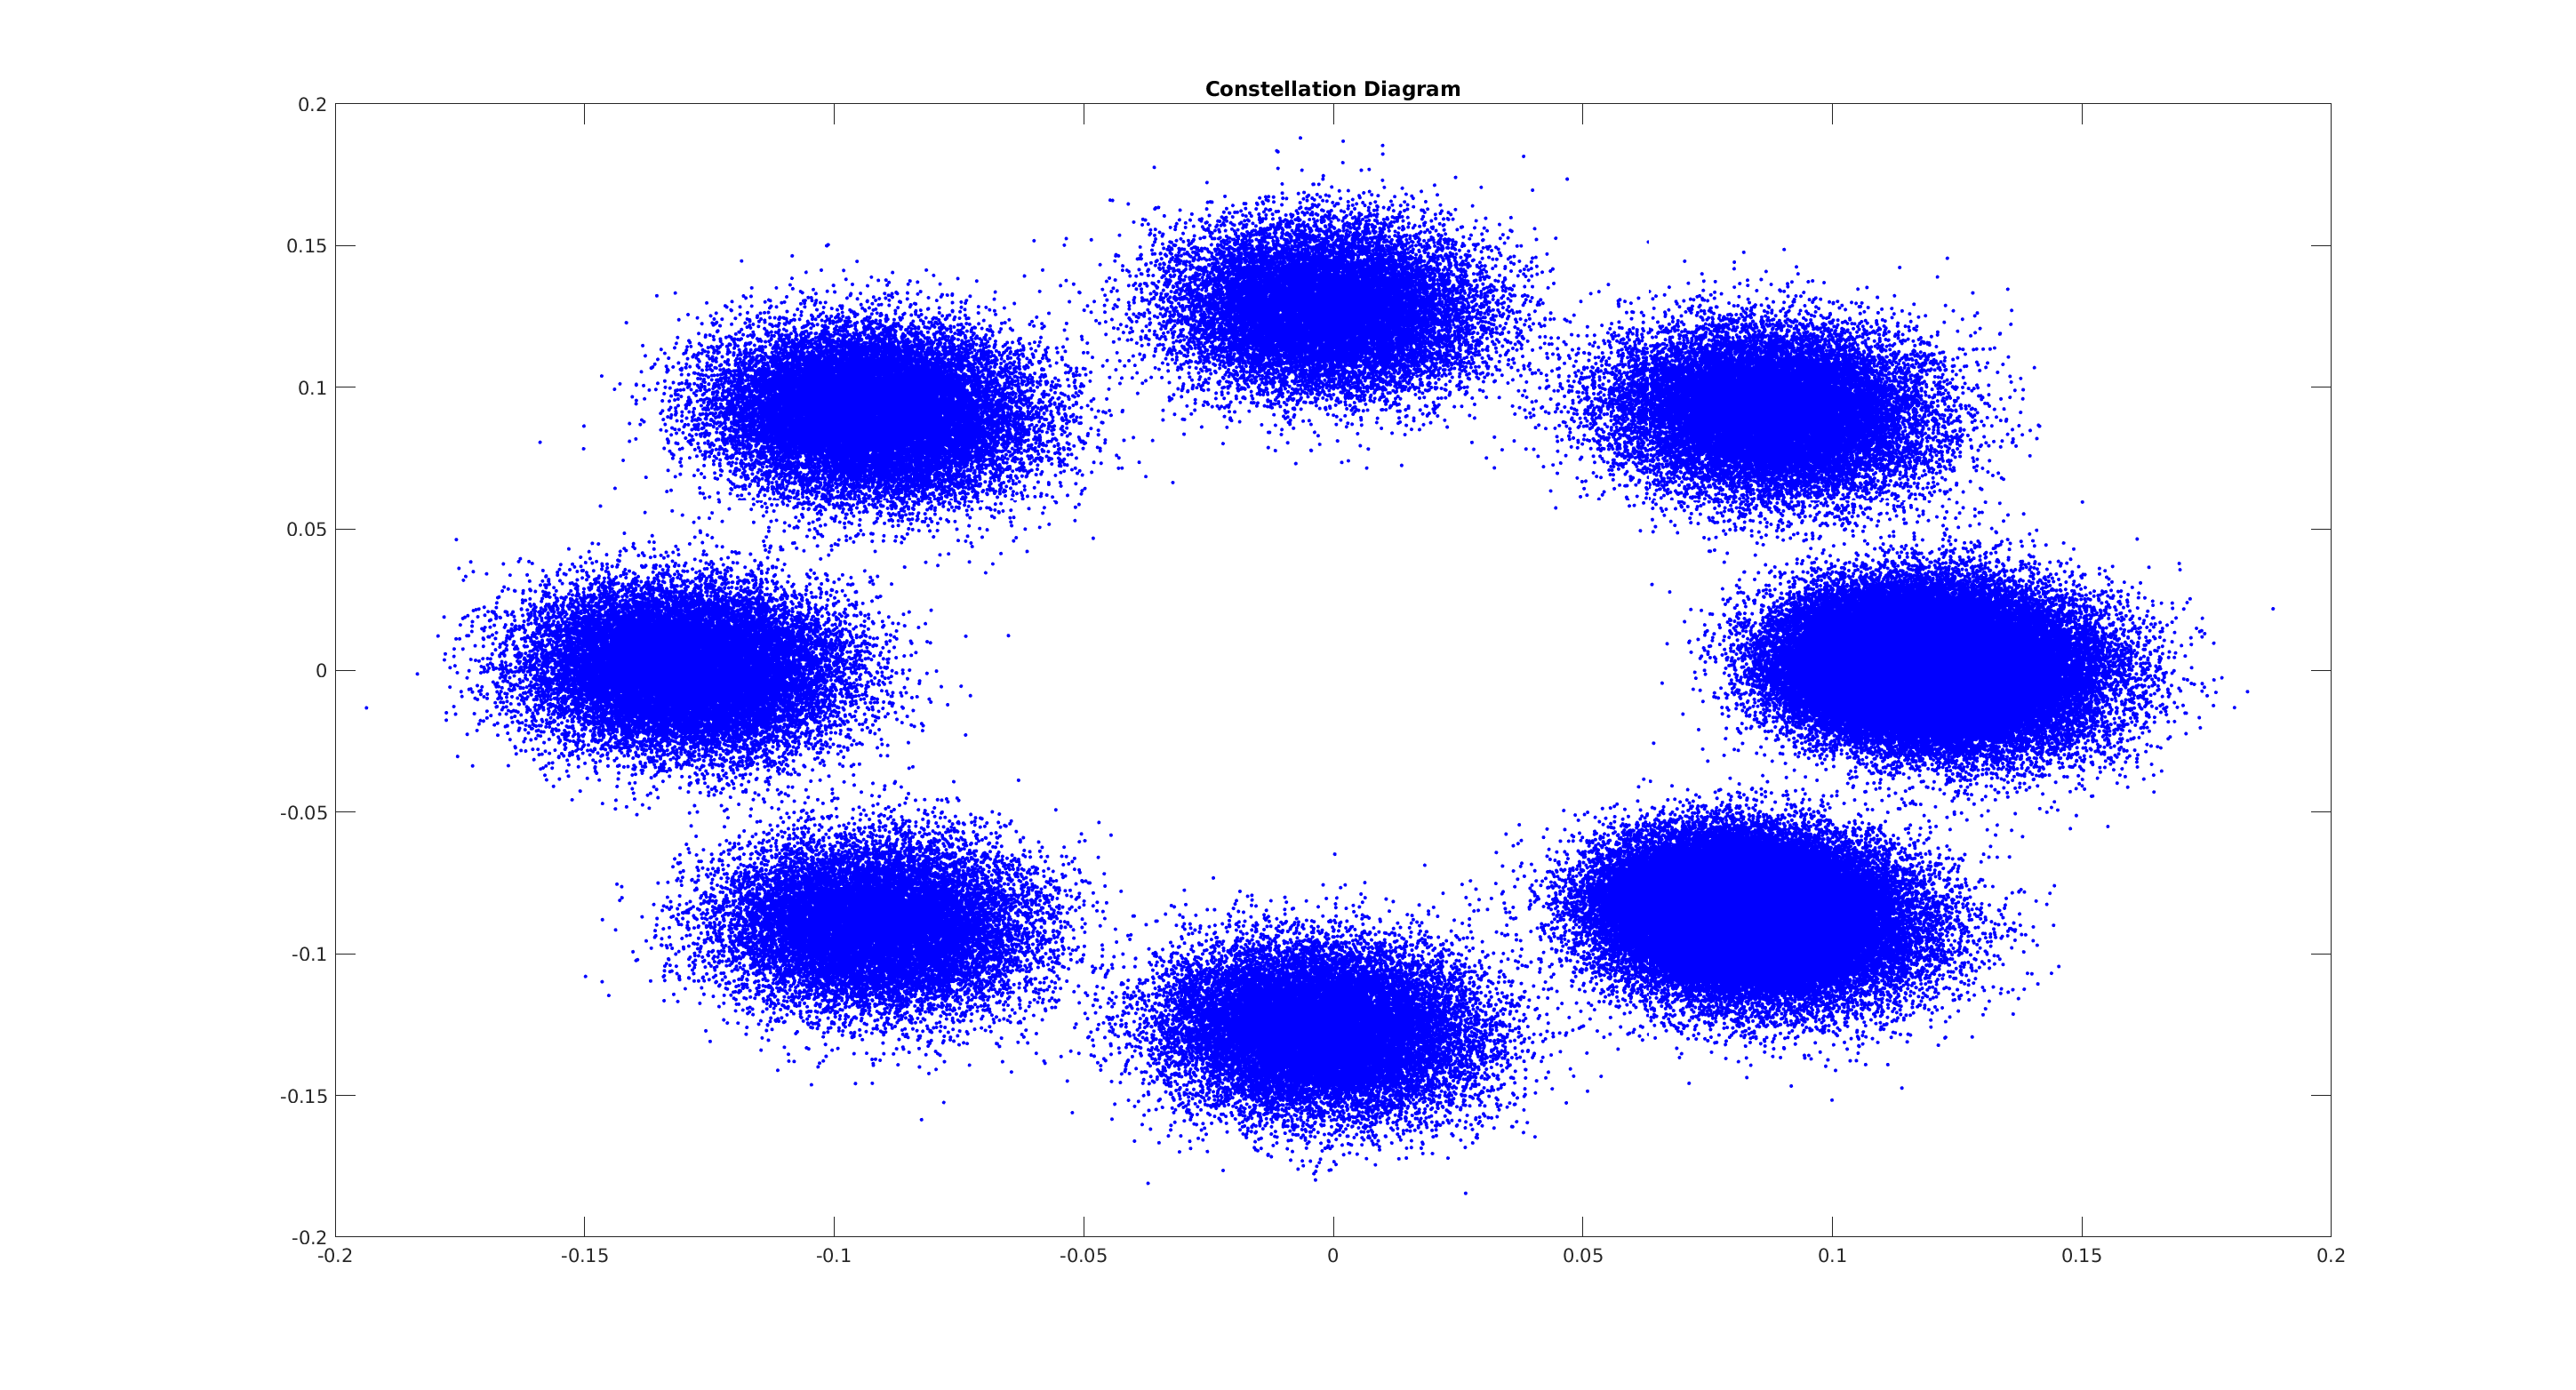
\includegraphics[width = \columnwidth]{constellation.png}
\end{figure}


符号判决采用距离比较的方法,将接收到的各个符号同8PSK的8个相位点求距离,取距离最小的点作为判决结果,得到星座图。由于是SNR=10时的图像,可以看到星座图较为明显地分为了8个密集区,对应8PSK的8个相位点。


\begin{figure}[H]
\centering
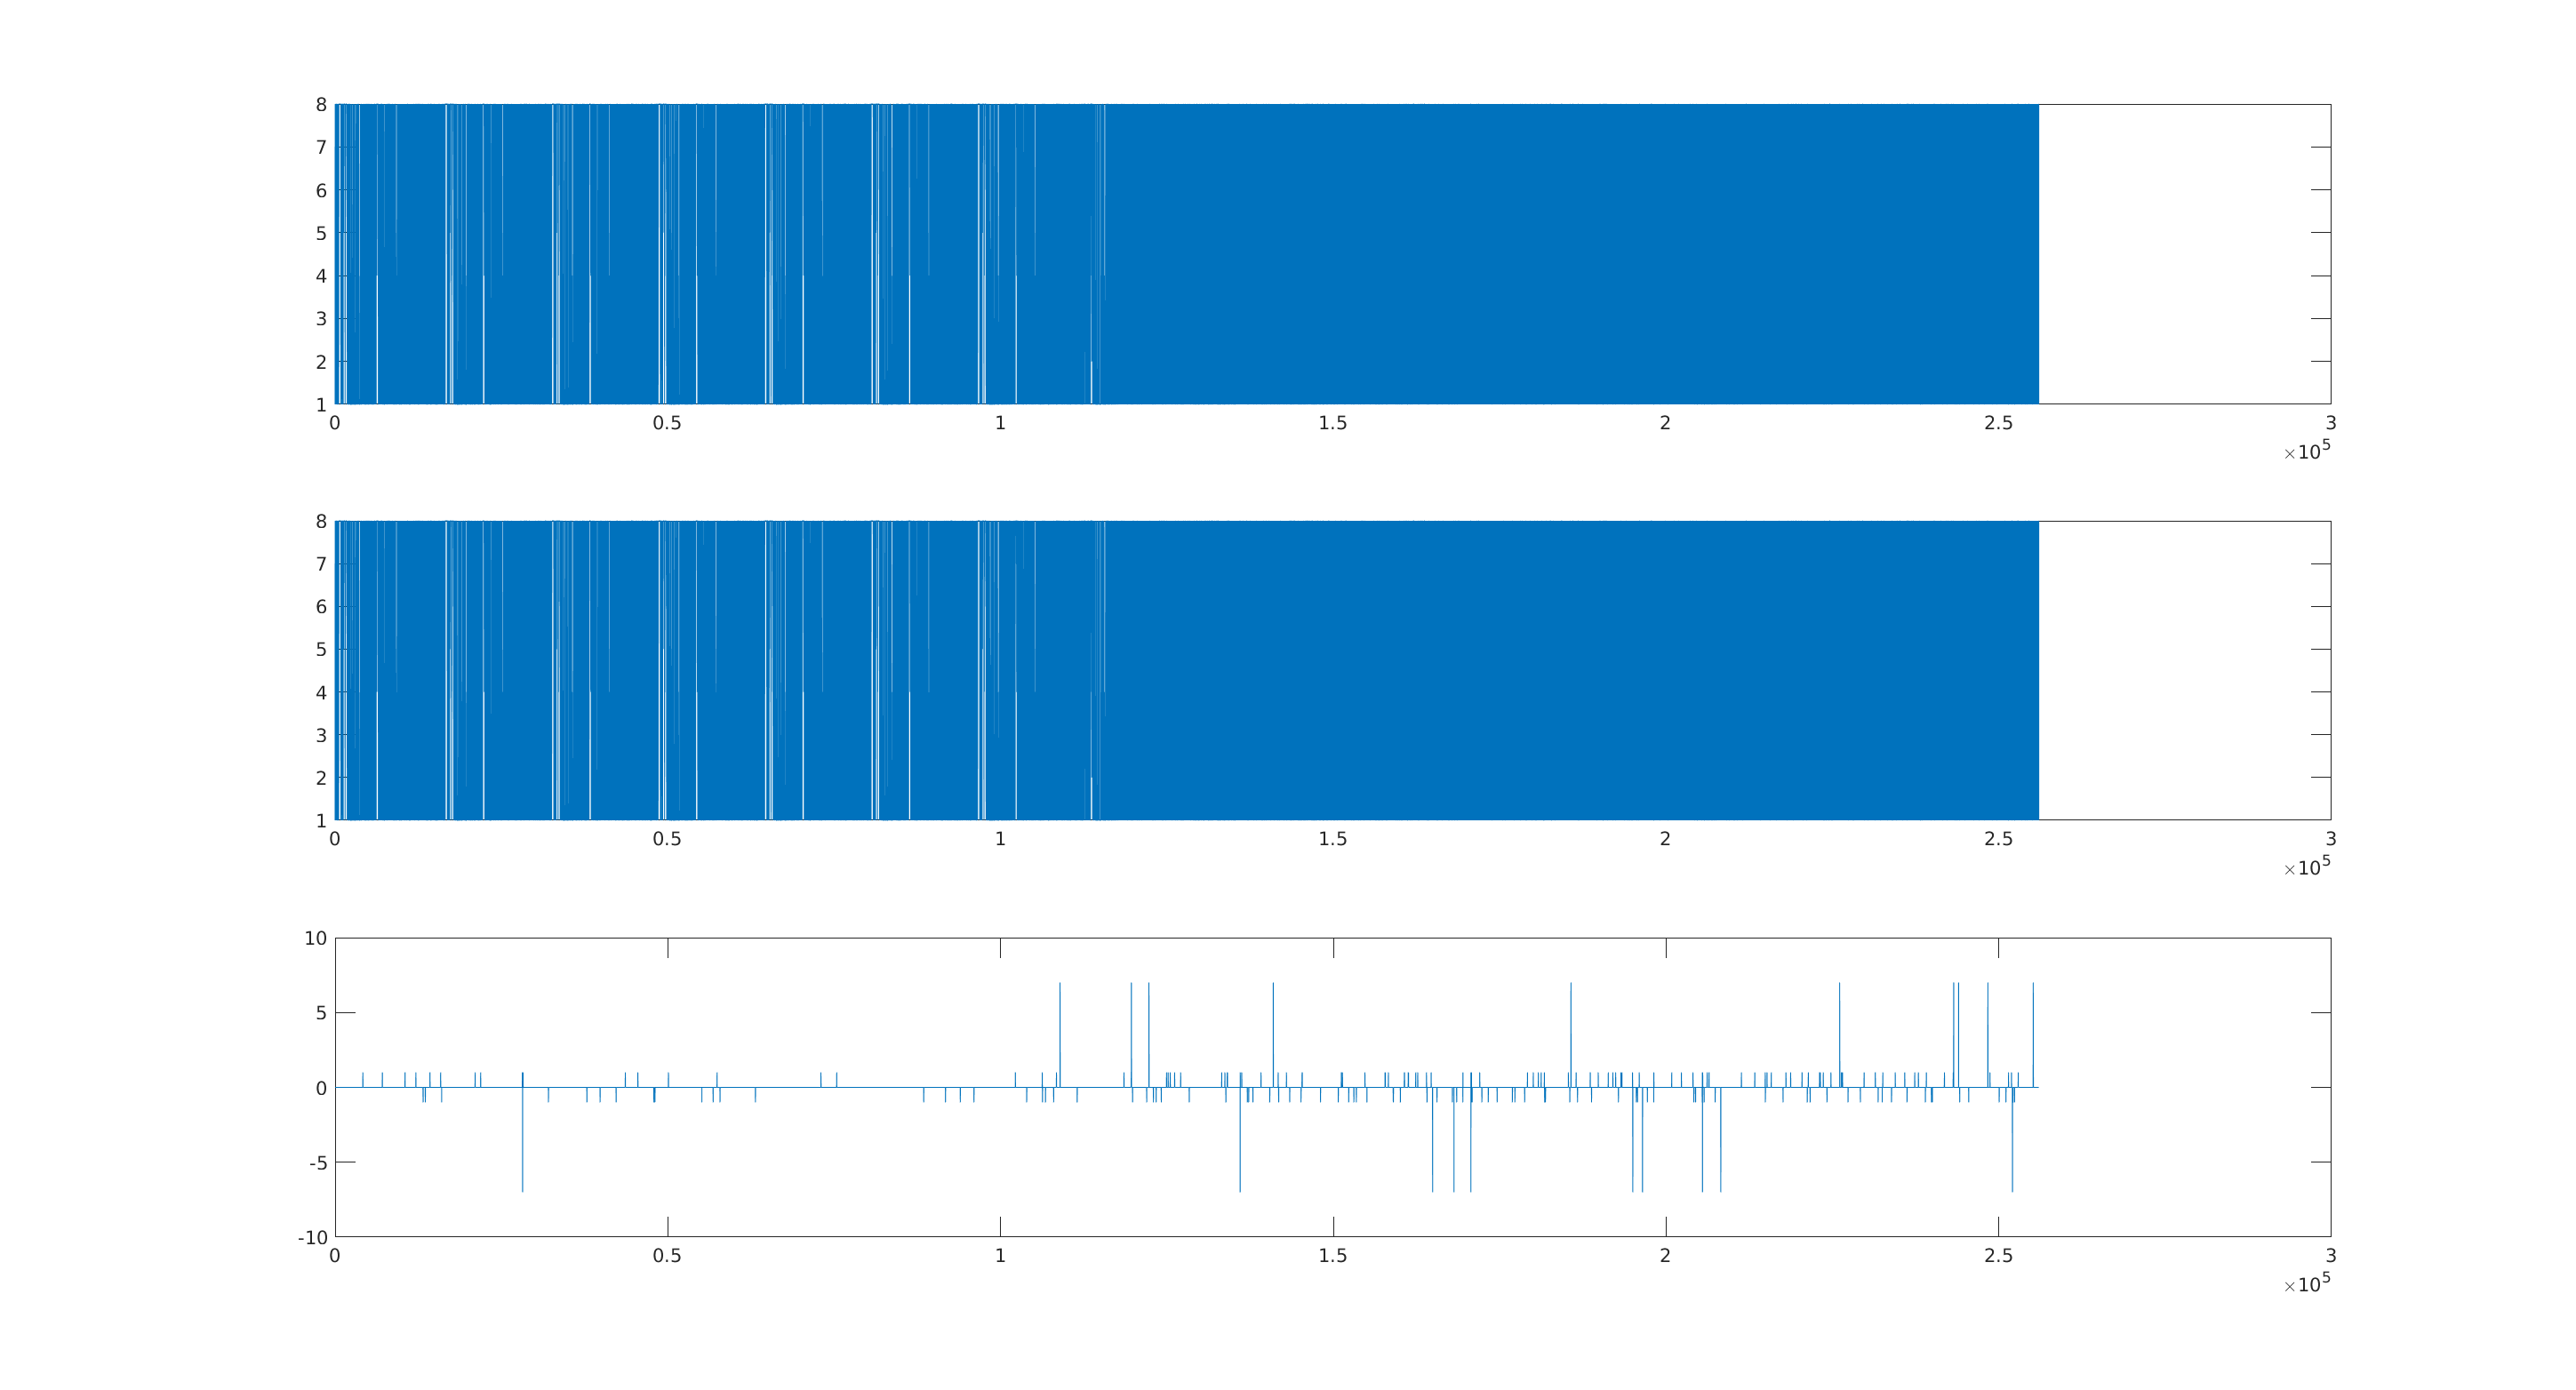
\includegraphics[width = \columnwidth]{error.png}
\end{figure}

同时做出发送比特序列和接收比特序列的图像,由于过于密集不够直观,故做出第三条图像,为二者差值,可以看到存在少量的错判。

\subsection{误码率计算}

\begin{lstlisting}
    % Calculate
    
    bits_error = abs(bits_result-bits);
    BER = [BER biterr(bits, bits_result)];
    
end

% display and save
figure(10)
hold off;
BE = BER;
BER = BER / (3 * length(bits));
plot(10 * log10(Es_range/(K * N0)) , 10 * log10(BER), 'b');
hold on;
% plot the theoretical curve
plot(bers0.data{1,1}, 10 * log10(bers0.data{1,2}), 'r');
title('BER(dB)-EbN0(dB)')
legend('simulate result', 'theoretical calculation');
saveas(10, [basepath 'figure/BER-EBN0.png']);
\end{lstlisting}

\begin{figure}[H]
\centering
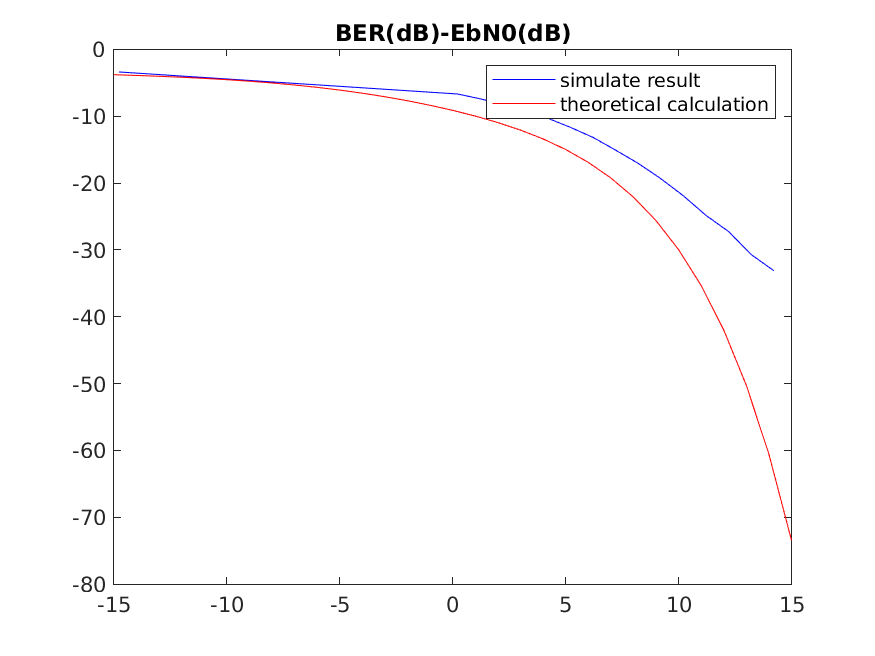
\includegraphics[width = \columnwidth]{BER-EBN0.png}
\end{figure}

最后的误码率曲线采用对数坐标,可以看到当EbN0较低时,仿真结果与理论曲线吻合较好,但当EbN0大于10dB时,两条曲线有数量级的差距,仿真结果明显差于理想曲线。

结合滤波器的时域、频域曲线分析可知,在这种设计下的滤波器存在较强的符号间干扰,随着噪声的逐渐减小,符号间干扰的作用越来越明显,显著影响到判决结果。

\section{比较与分析}

以上是对整个流程的简单介绍,下面针对不同信噪比、不同滤波器得到的结果进行比较和分析。

\subsection{信噪比的影响}

由星座图可以比较明显直观地看到SNR对于信道性能的影响。

\begin{figure}[H]
\begin{minipage}[t]{0.5\linewidth}
\centering
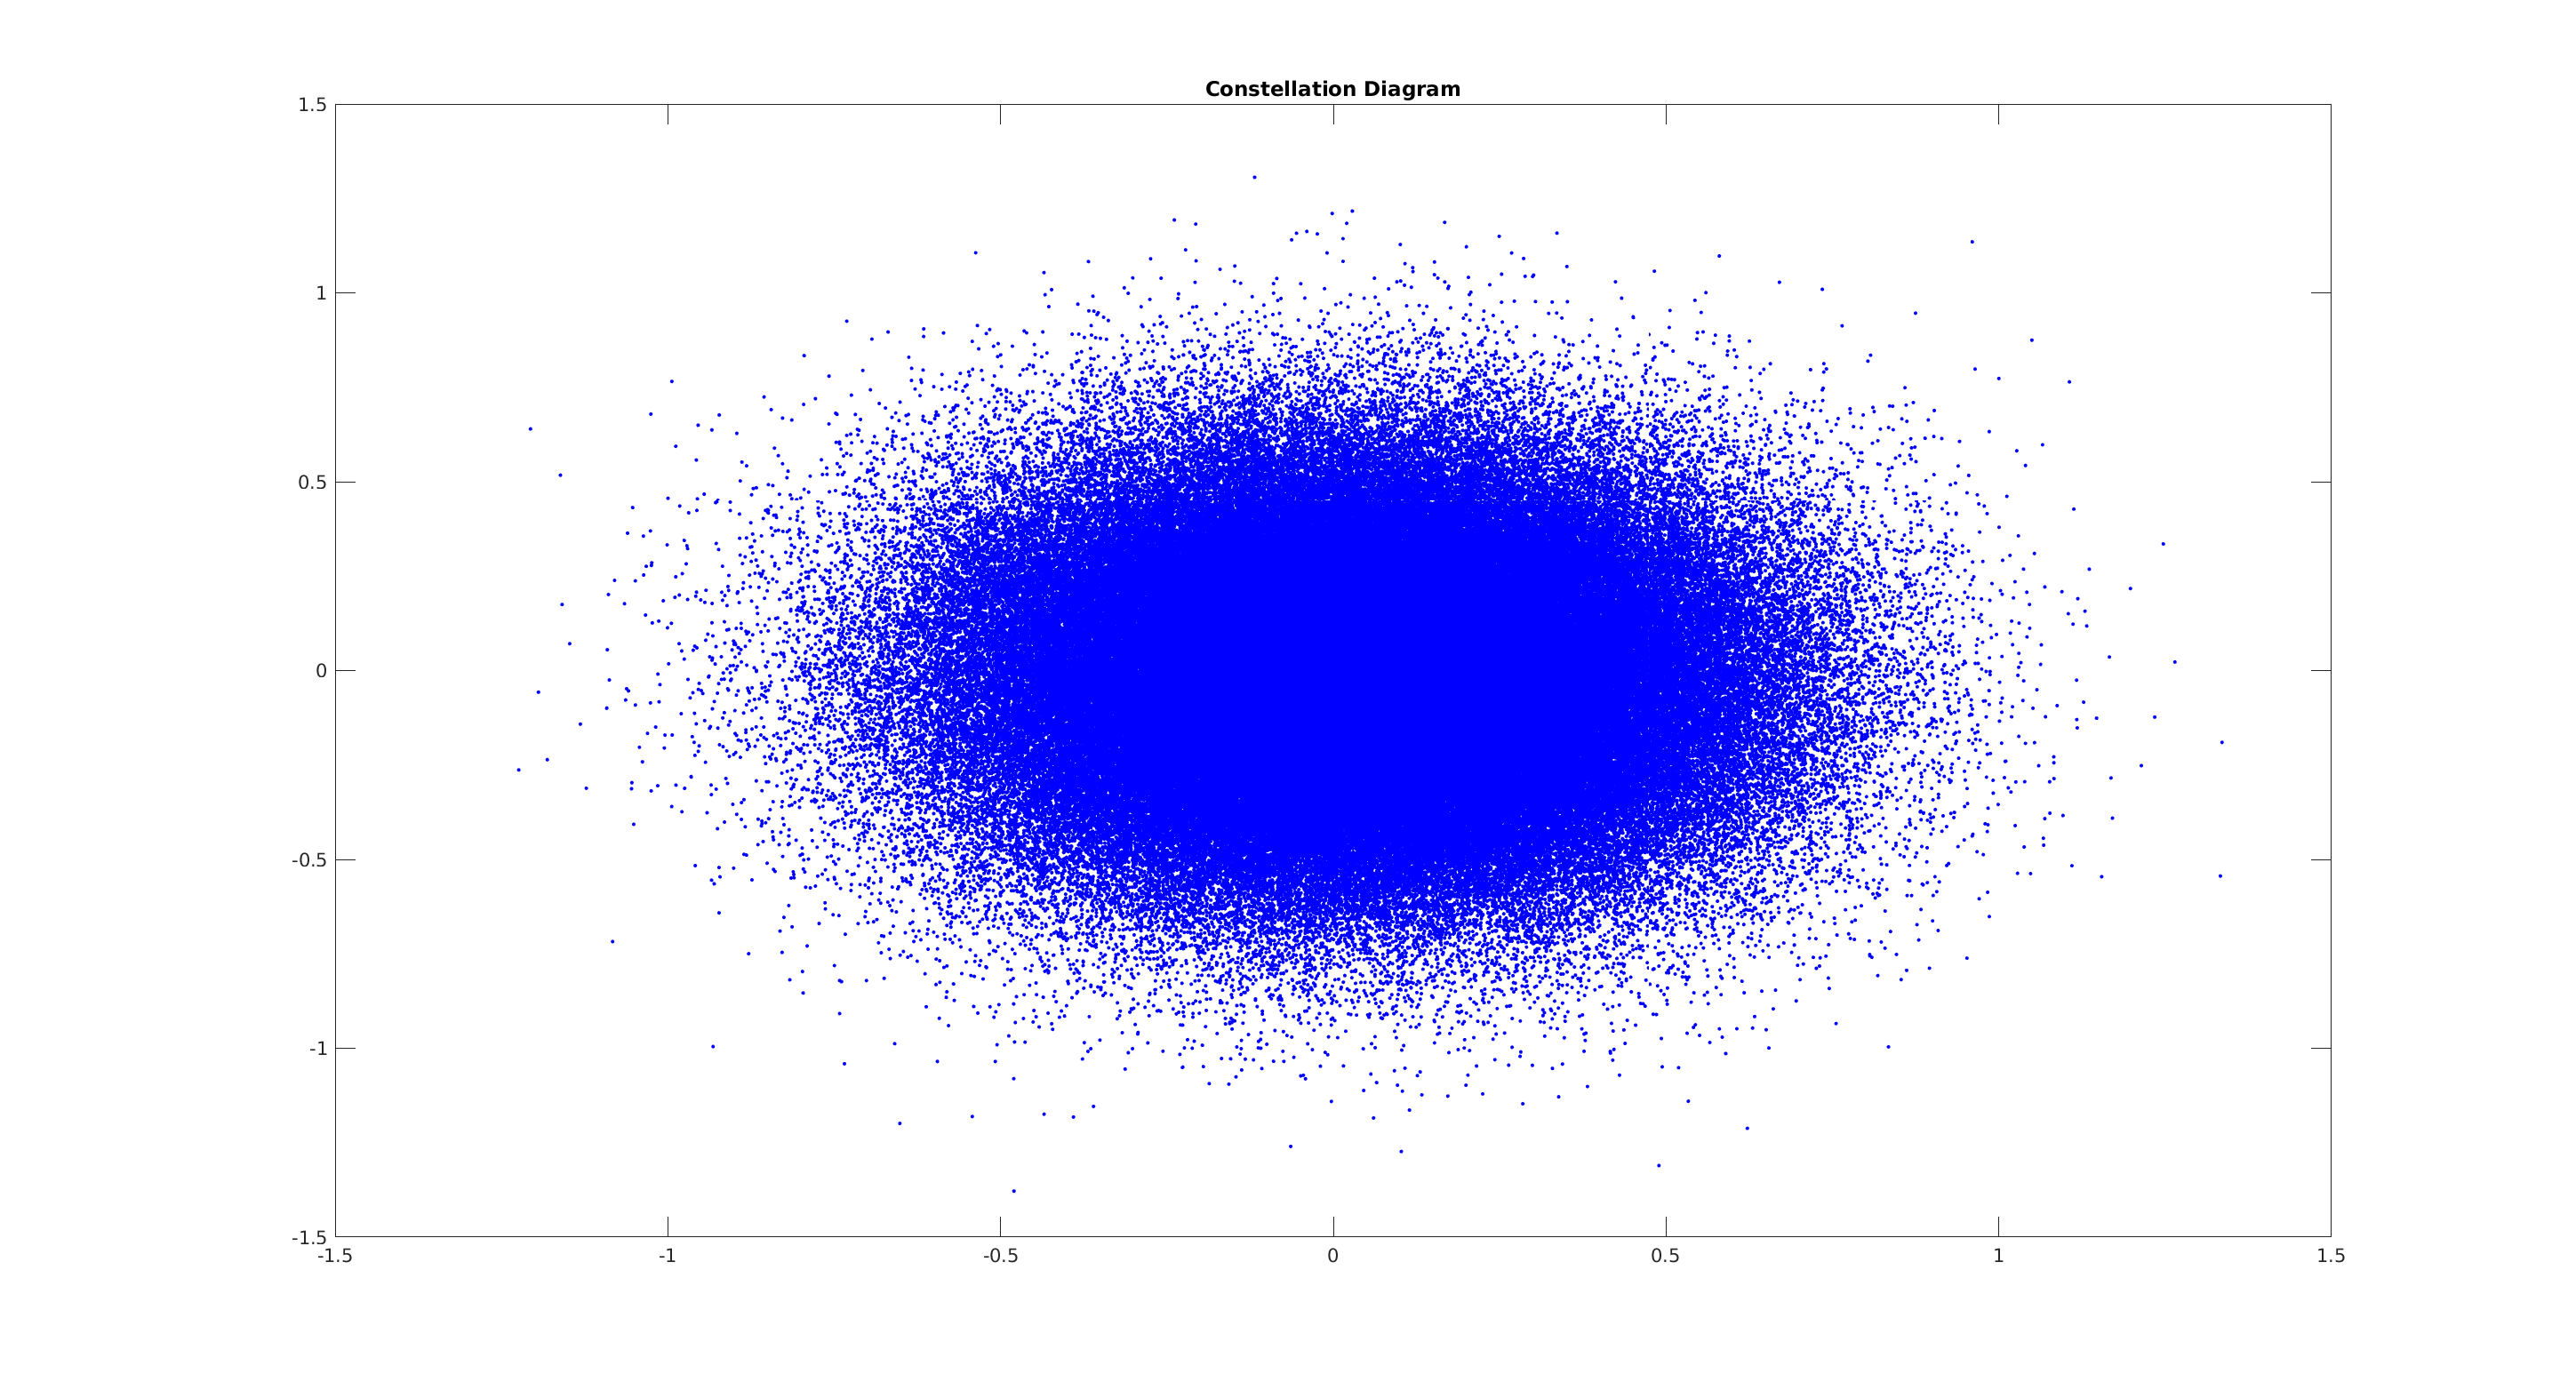
\includegraphics[width=0.9\columnwidth]{constellation1.png}
\caption{SNR=-19dB}
\end{minipage}
\hfill
\begin{minipage}[t]{0.5\linewidth}
\centering
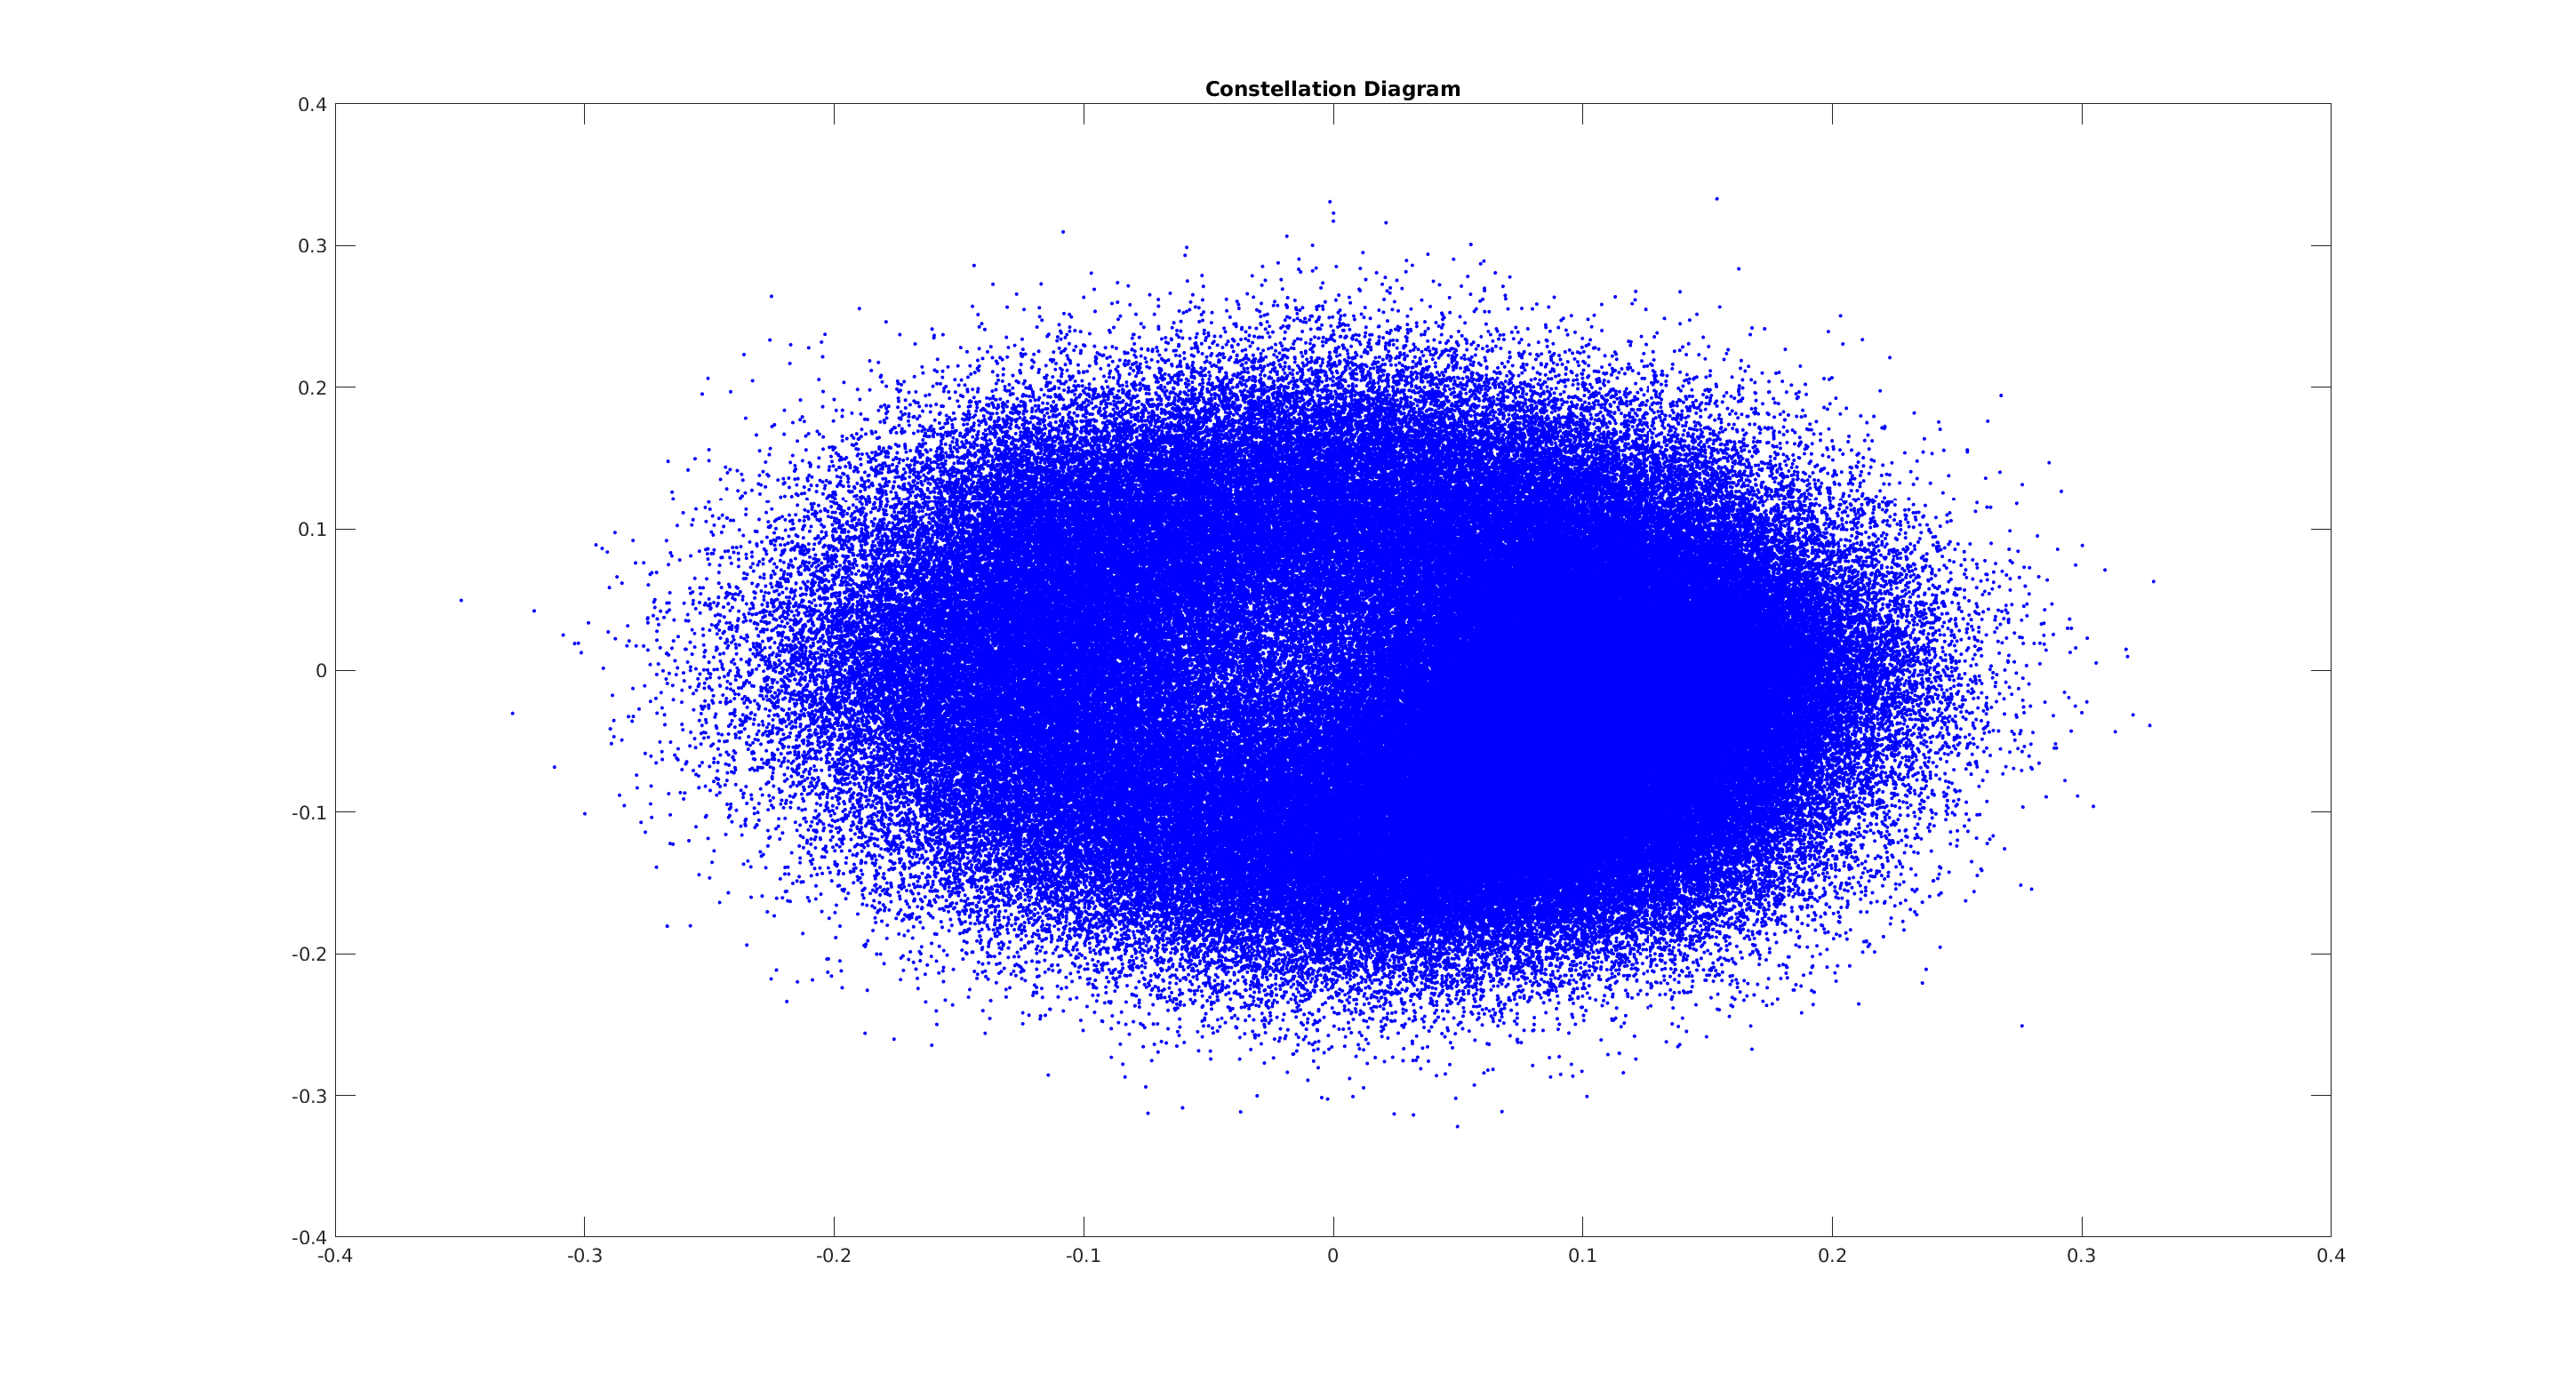
\includegraphics[width=0.9\columnwidth]{constellation2.png}
\caption{SNR=-4dB}
\end{minipage}
\end{figure}


\begin{figure}[H]
\begin{minipage}[t]{0.5\linewidth}
\centering
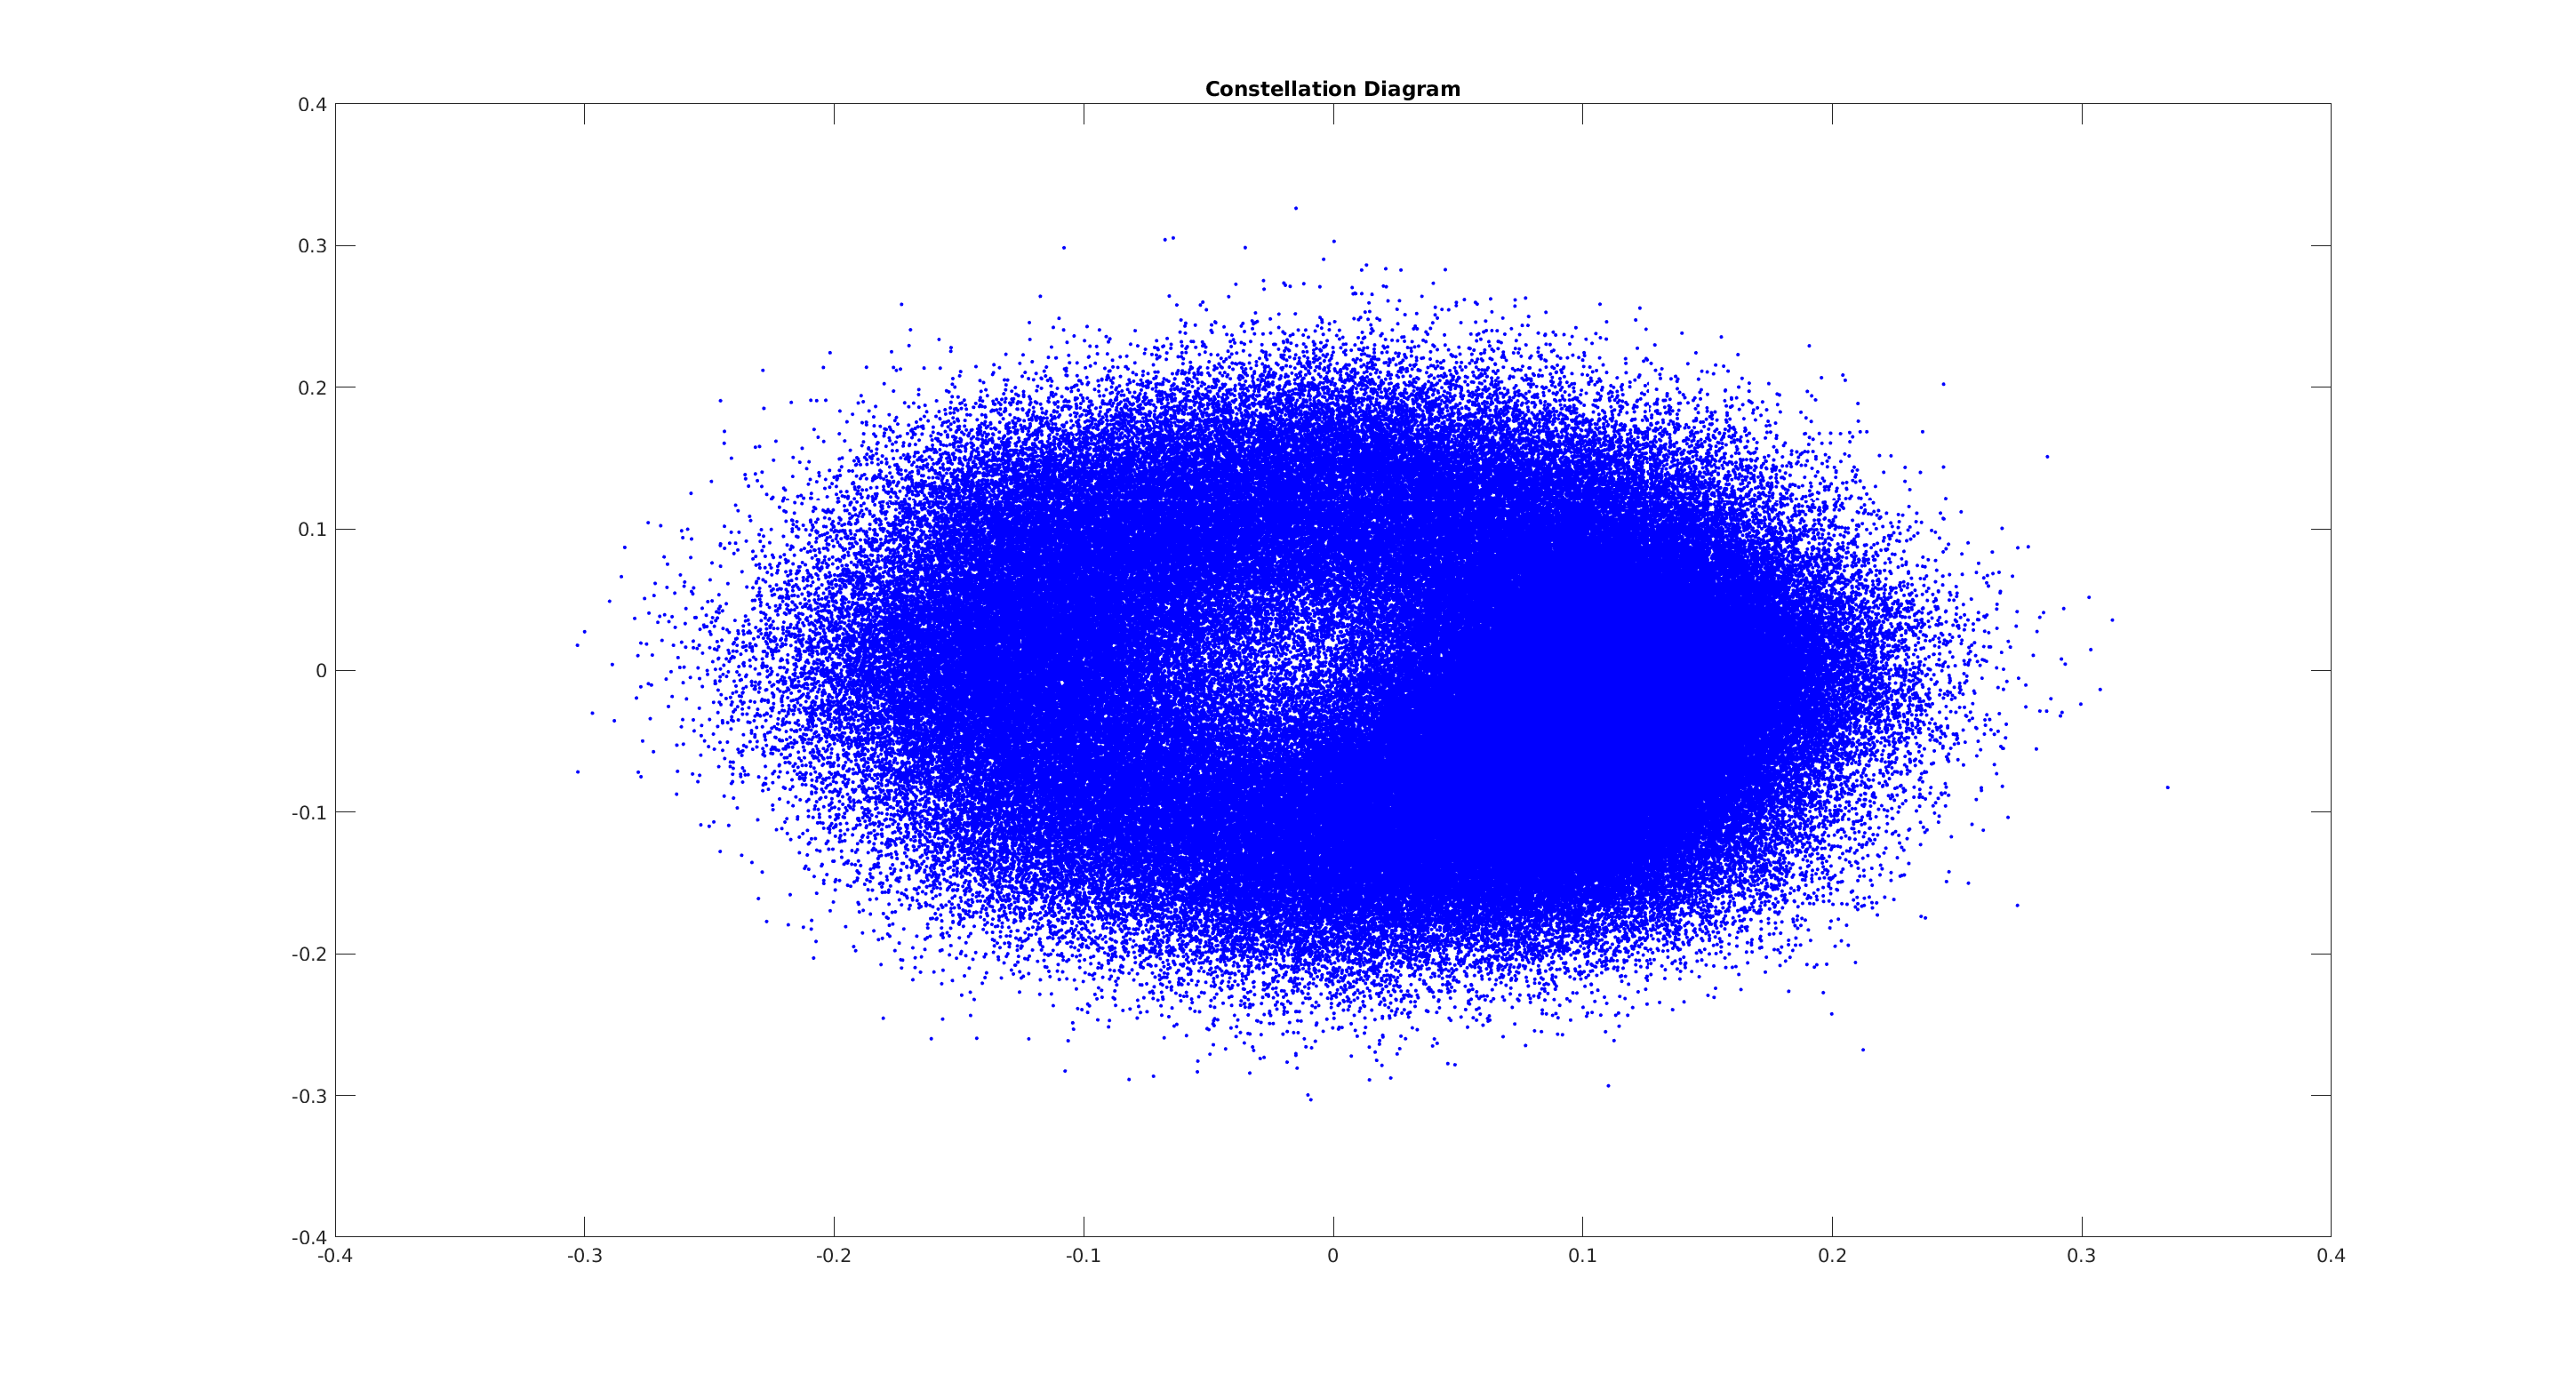
\includegraphics[width=0.9\columnwidth]{constellation3.png}
\caption{SNR=-3dB}
\end{minipage}
\hfill
\begin{minipage}[t]{0.5\linewidth}
\centering
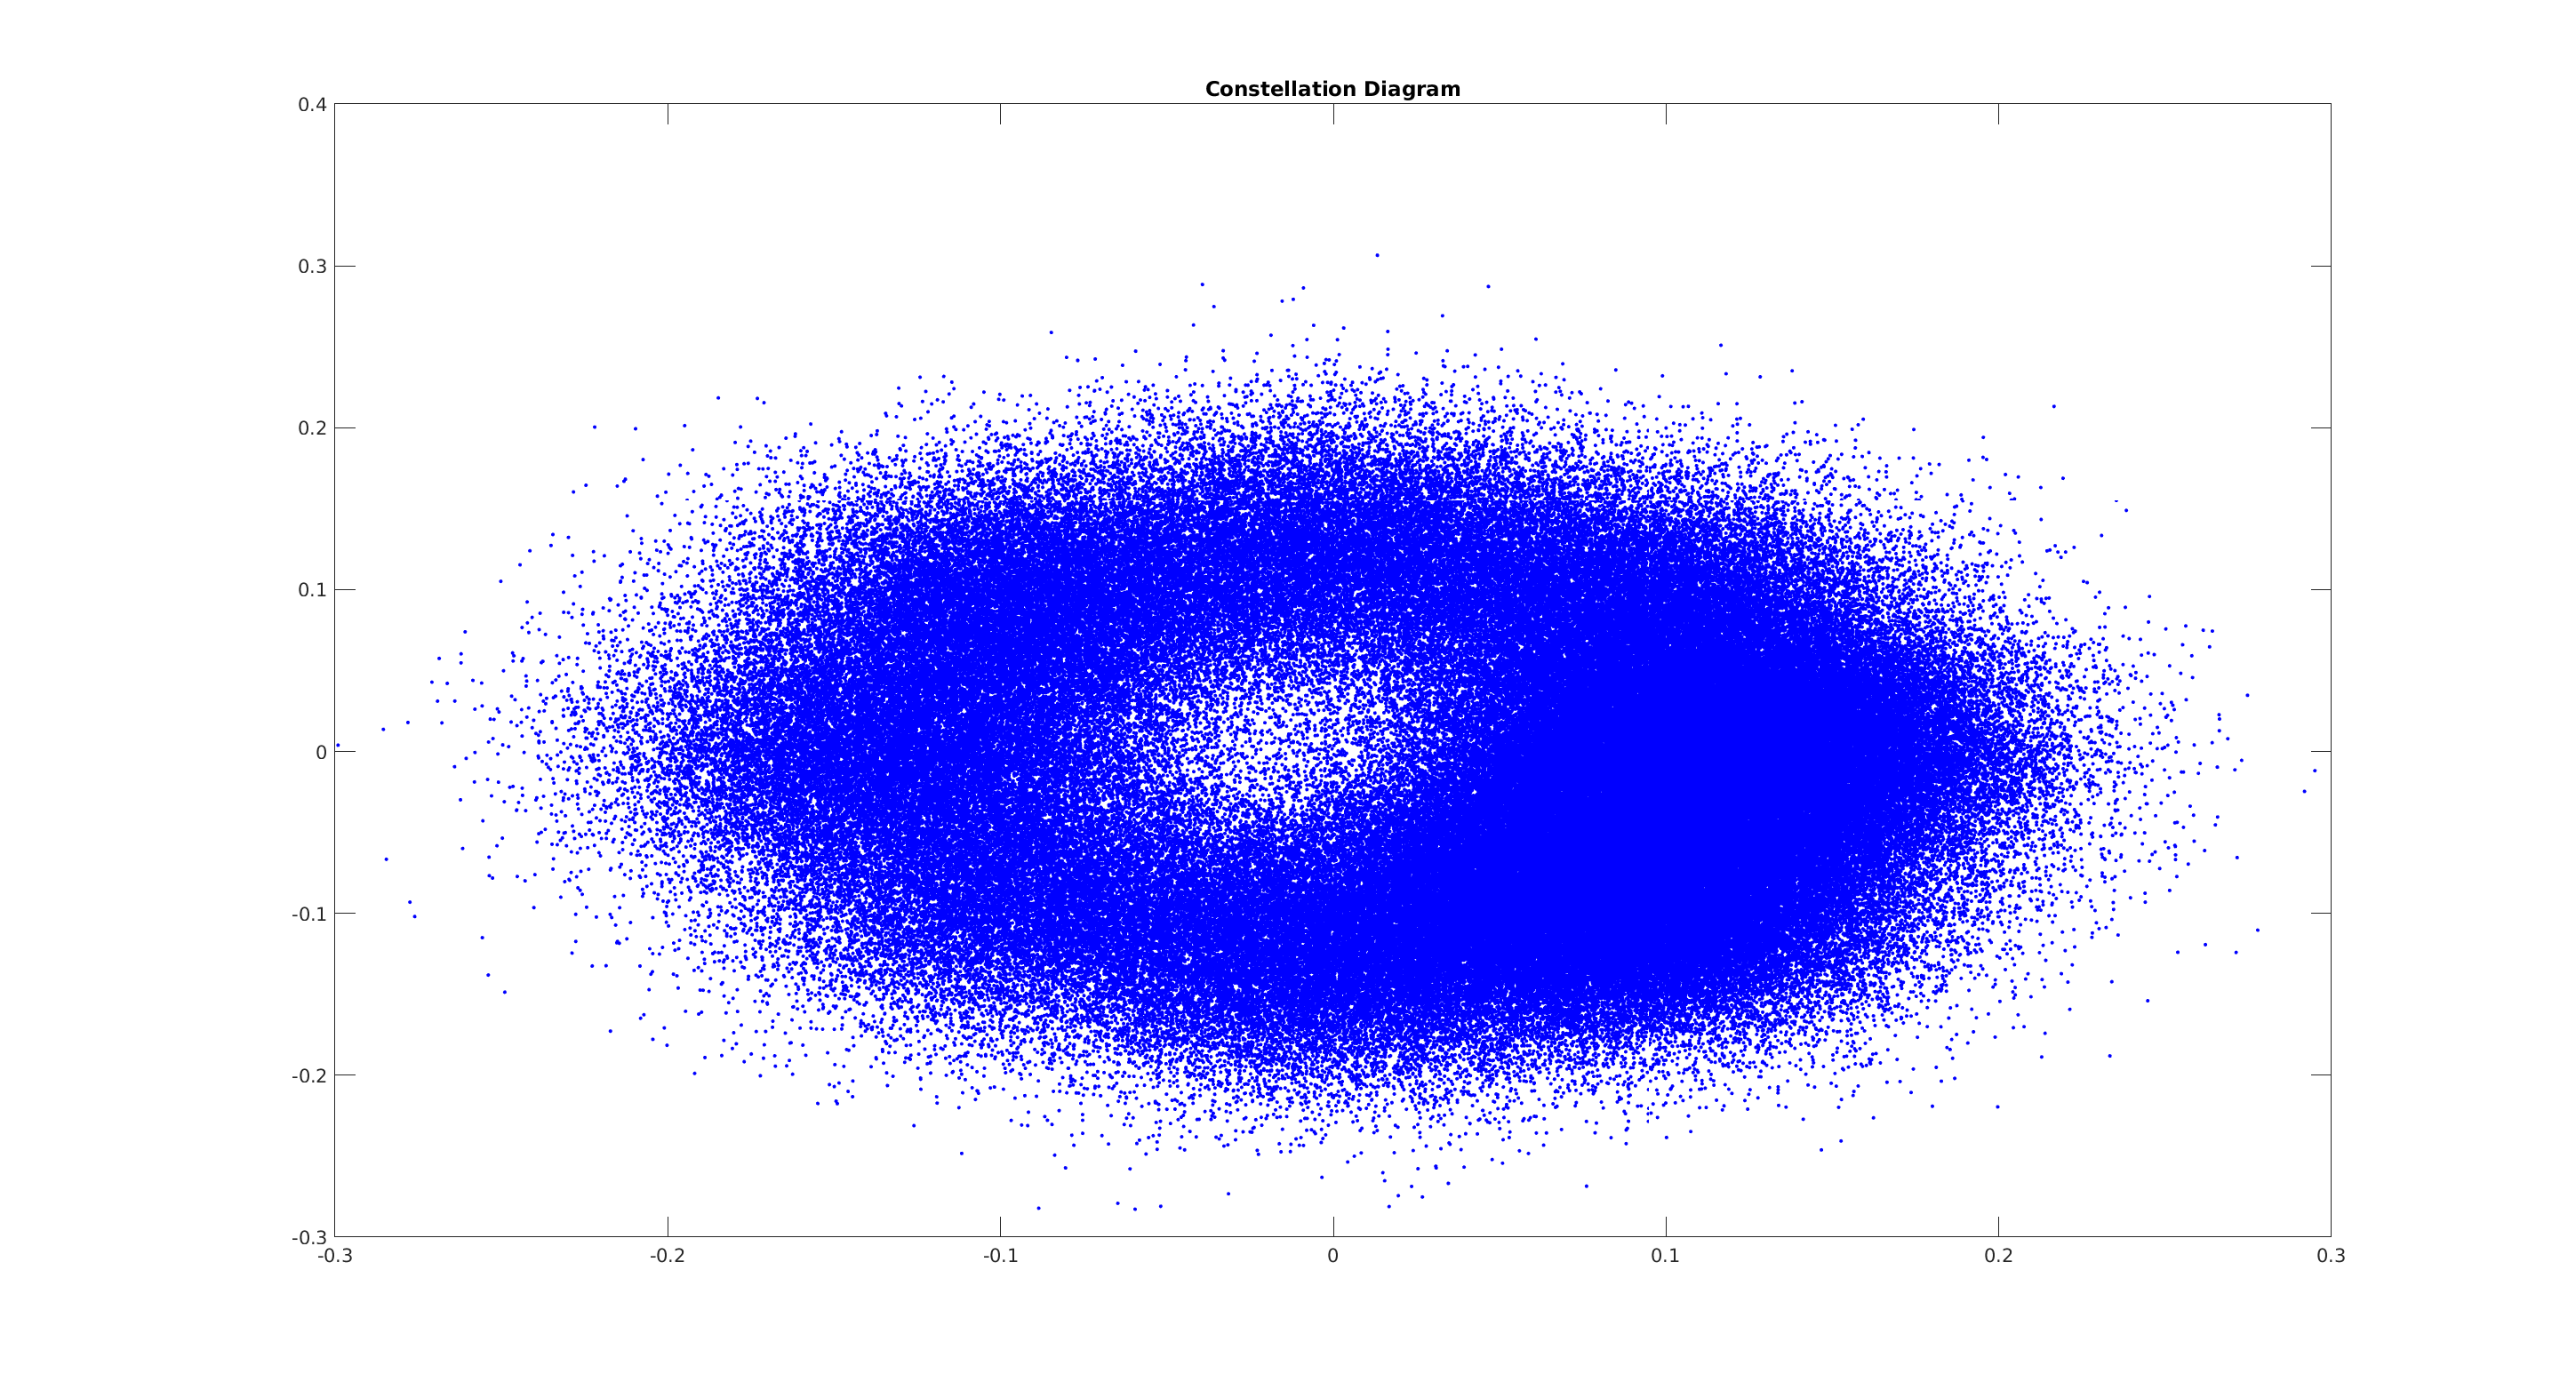
\includegraphics[width=0.9\columnwidth]{constellation4.png}
\caption{SNR=-2dB}
\end{minipage}
\end{figure}


\begin{figure}[H]
\begin{minipage}[t]{0.5\linewidth}
\centering
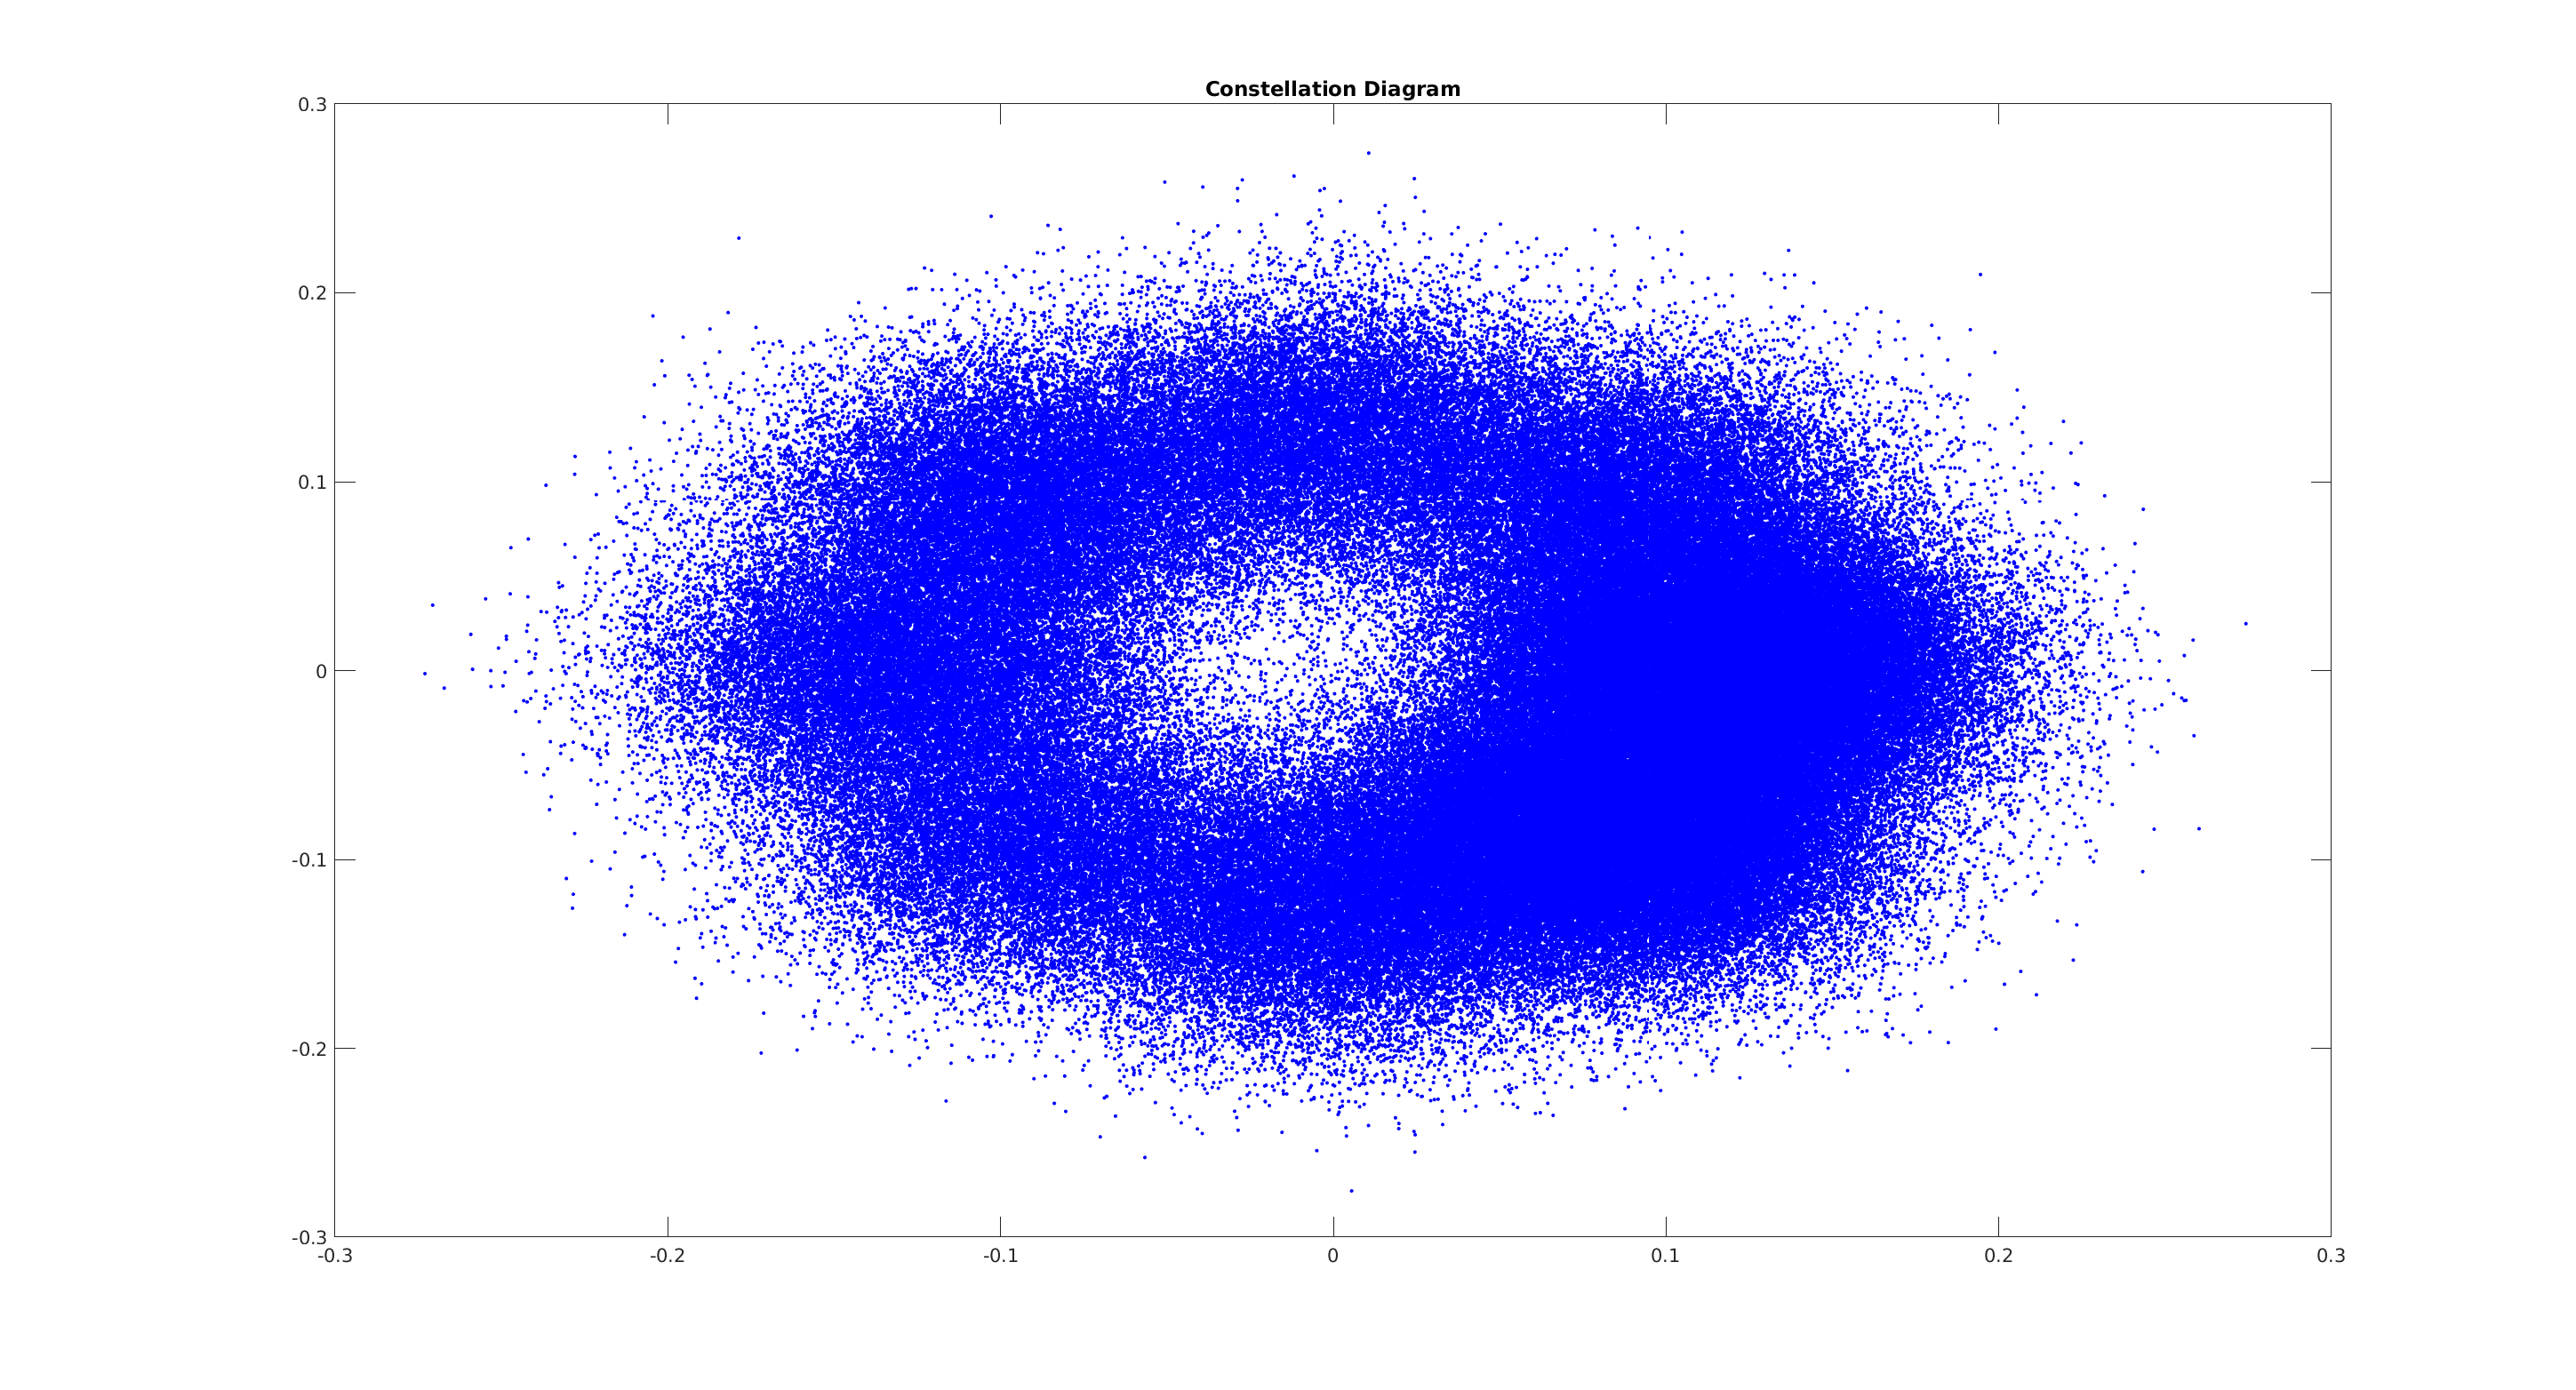
\includegraphics[width=0.9\columnwidth]{constellation5.png}
\caption{SNR=-1dB}
\end{minipage}
\hfill
\begin{minipage}[t]{0.5\linewidth}
\centering
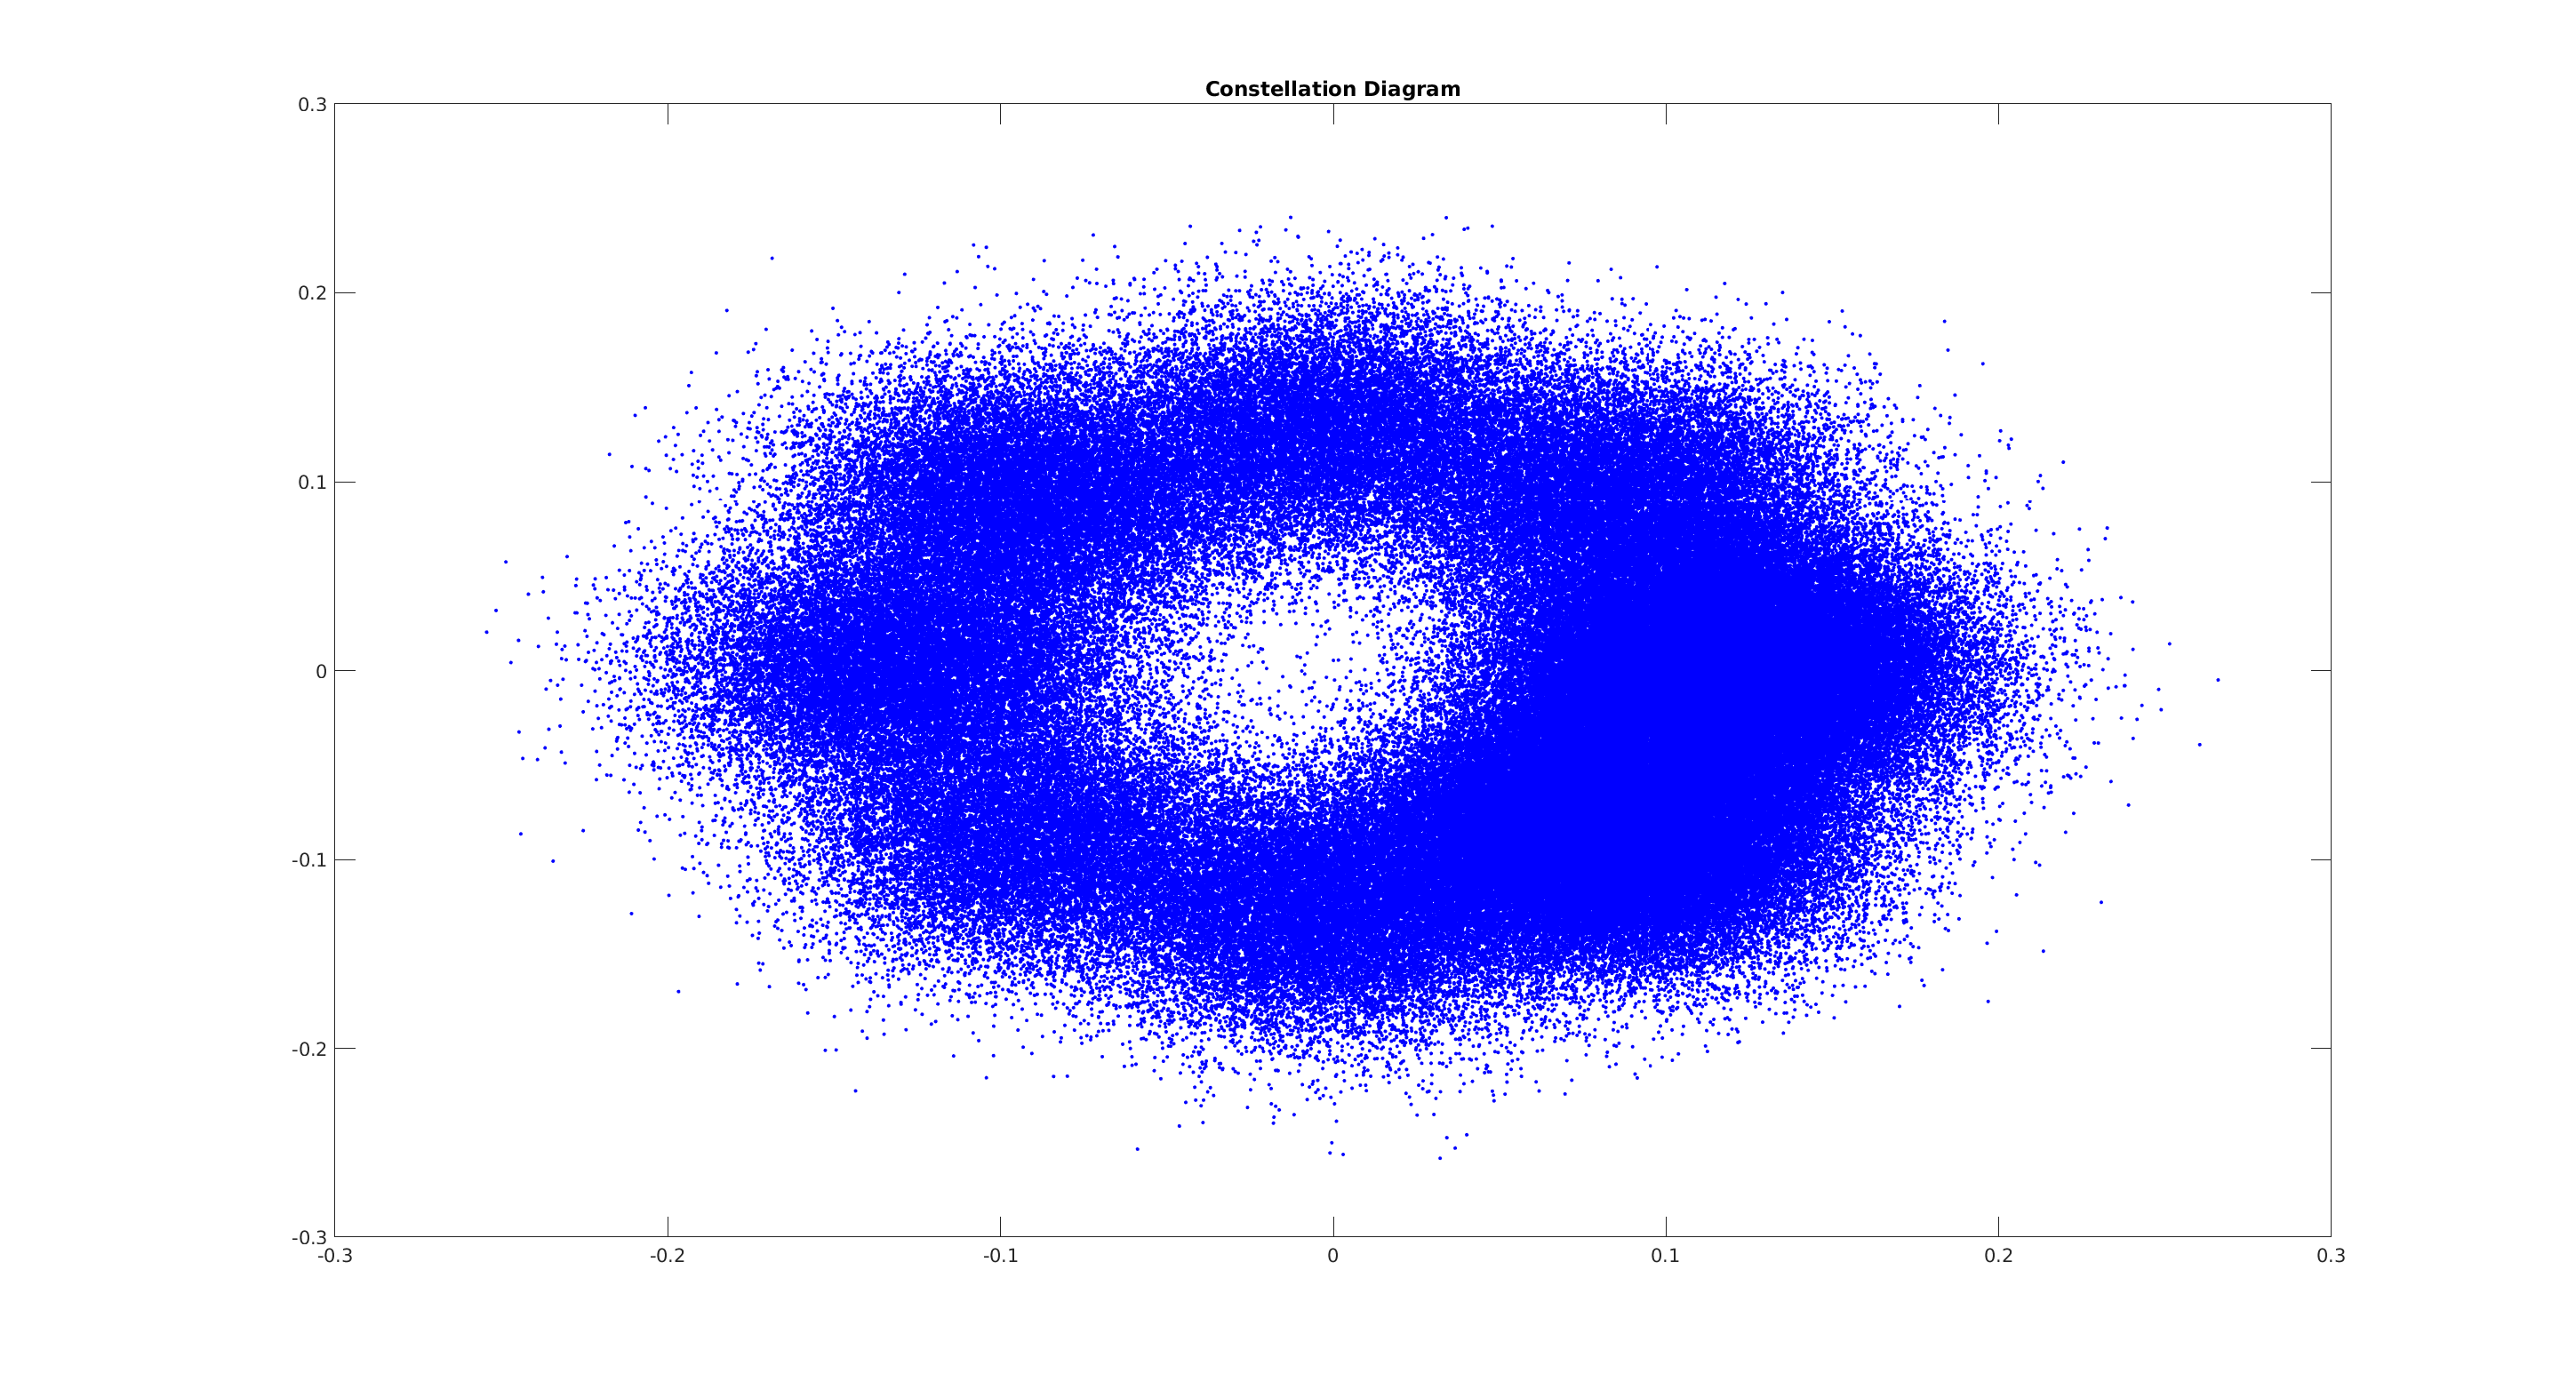
\includegraphics[width=0.9\columnwidth]{constellation6.png}
\caption{SNR=0dB}
\end{minipage}
\end{figure}


\begin{figure}[H]
\begin{minipage}[t]{0.5\linewidth}
\centering
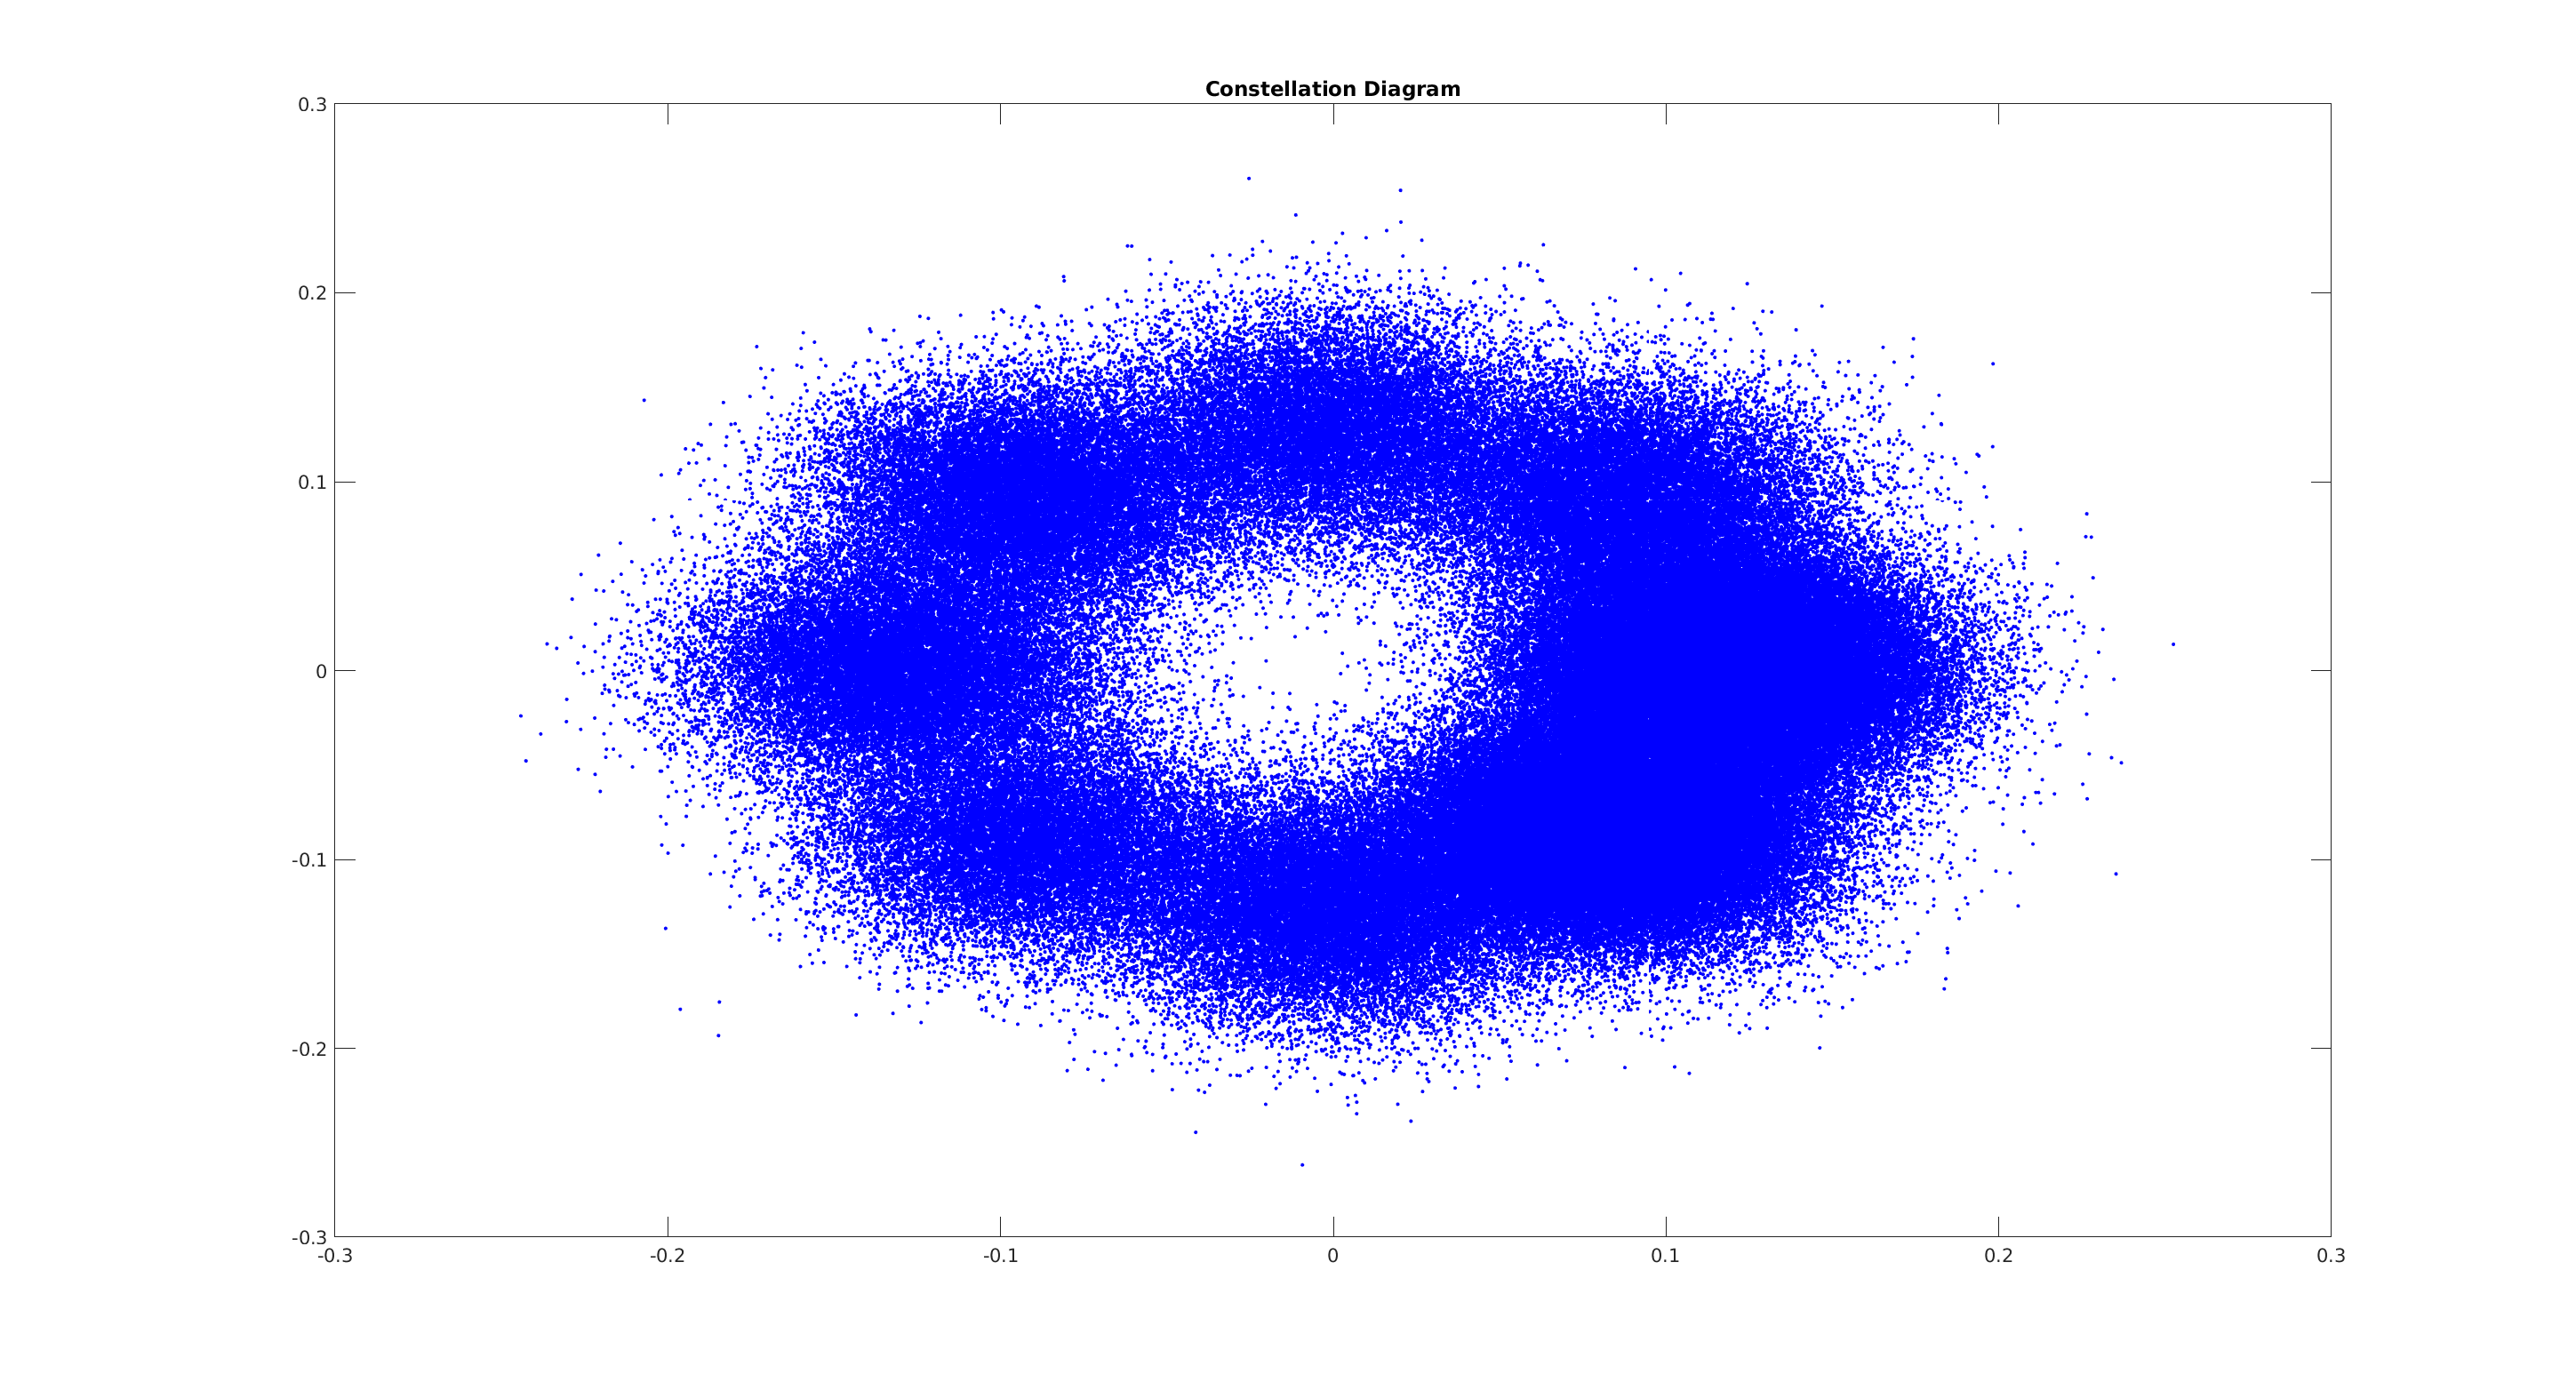
\includegraphics[width=0.9\columnwidth]{constellation7.png}
\caption{SNR=1dB}
\end{minipage}
\hfill
\begin{minipage}[t]{0.5\linewidth}
\centering
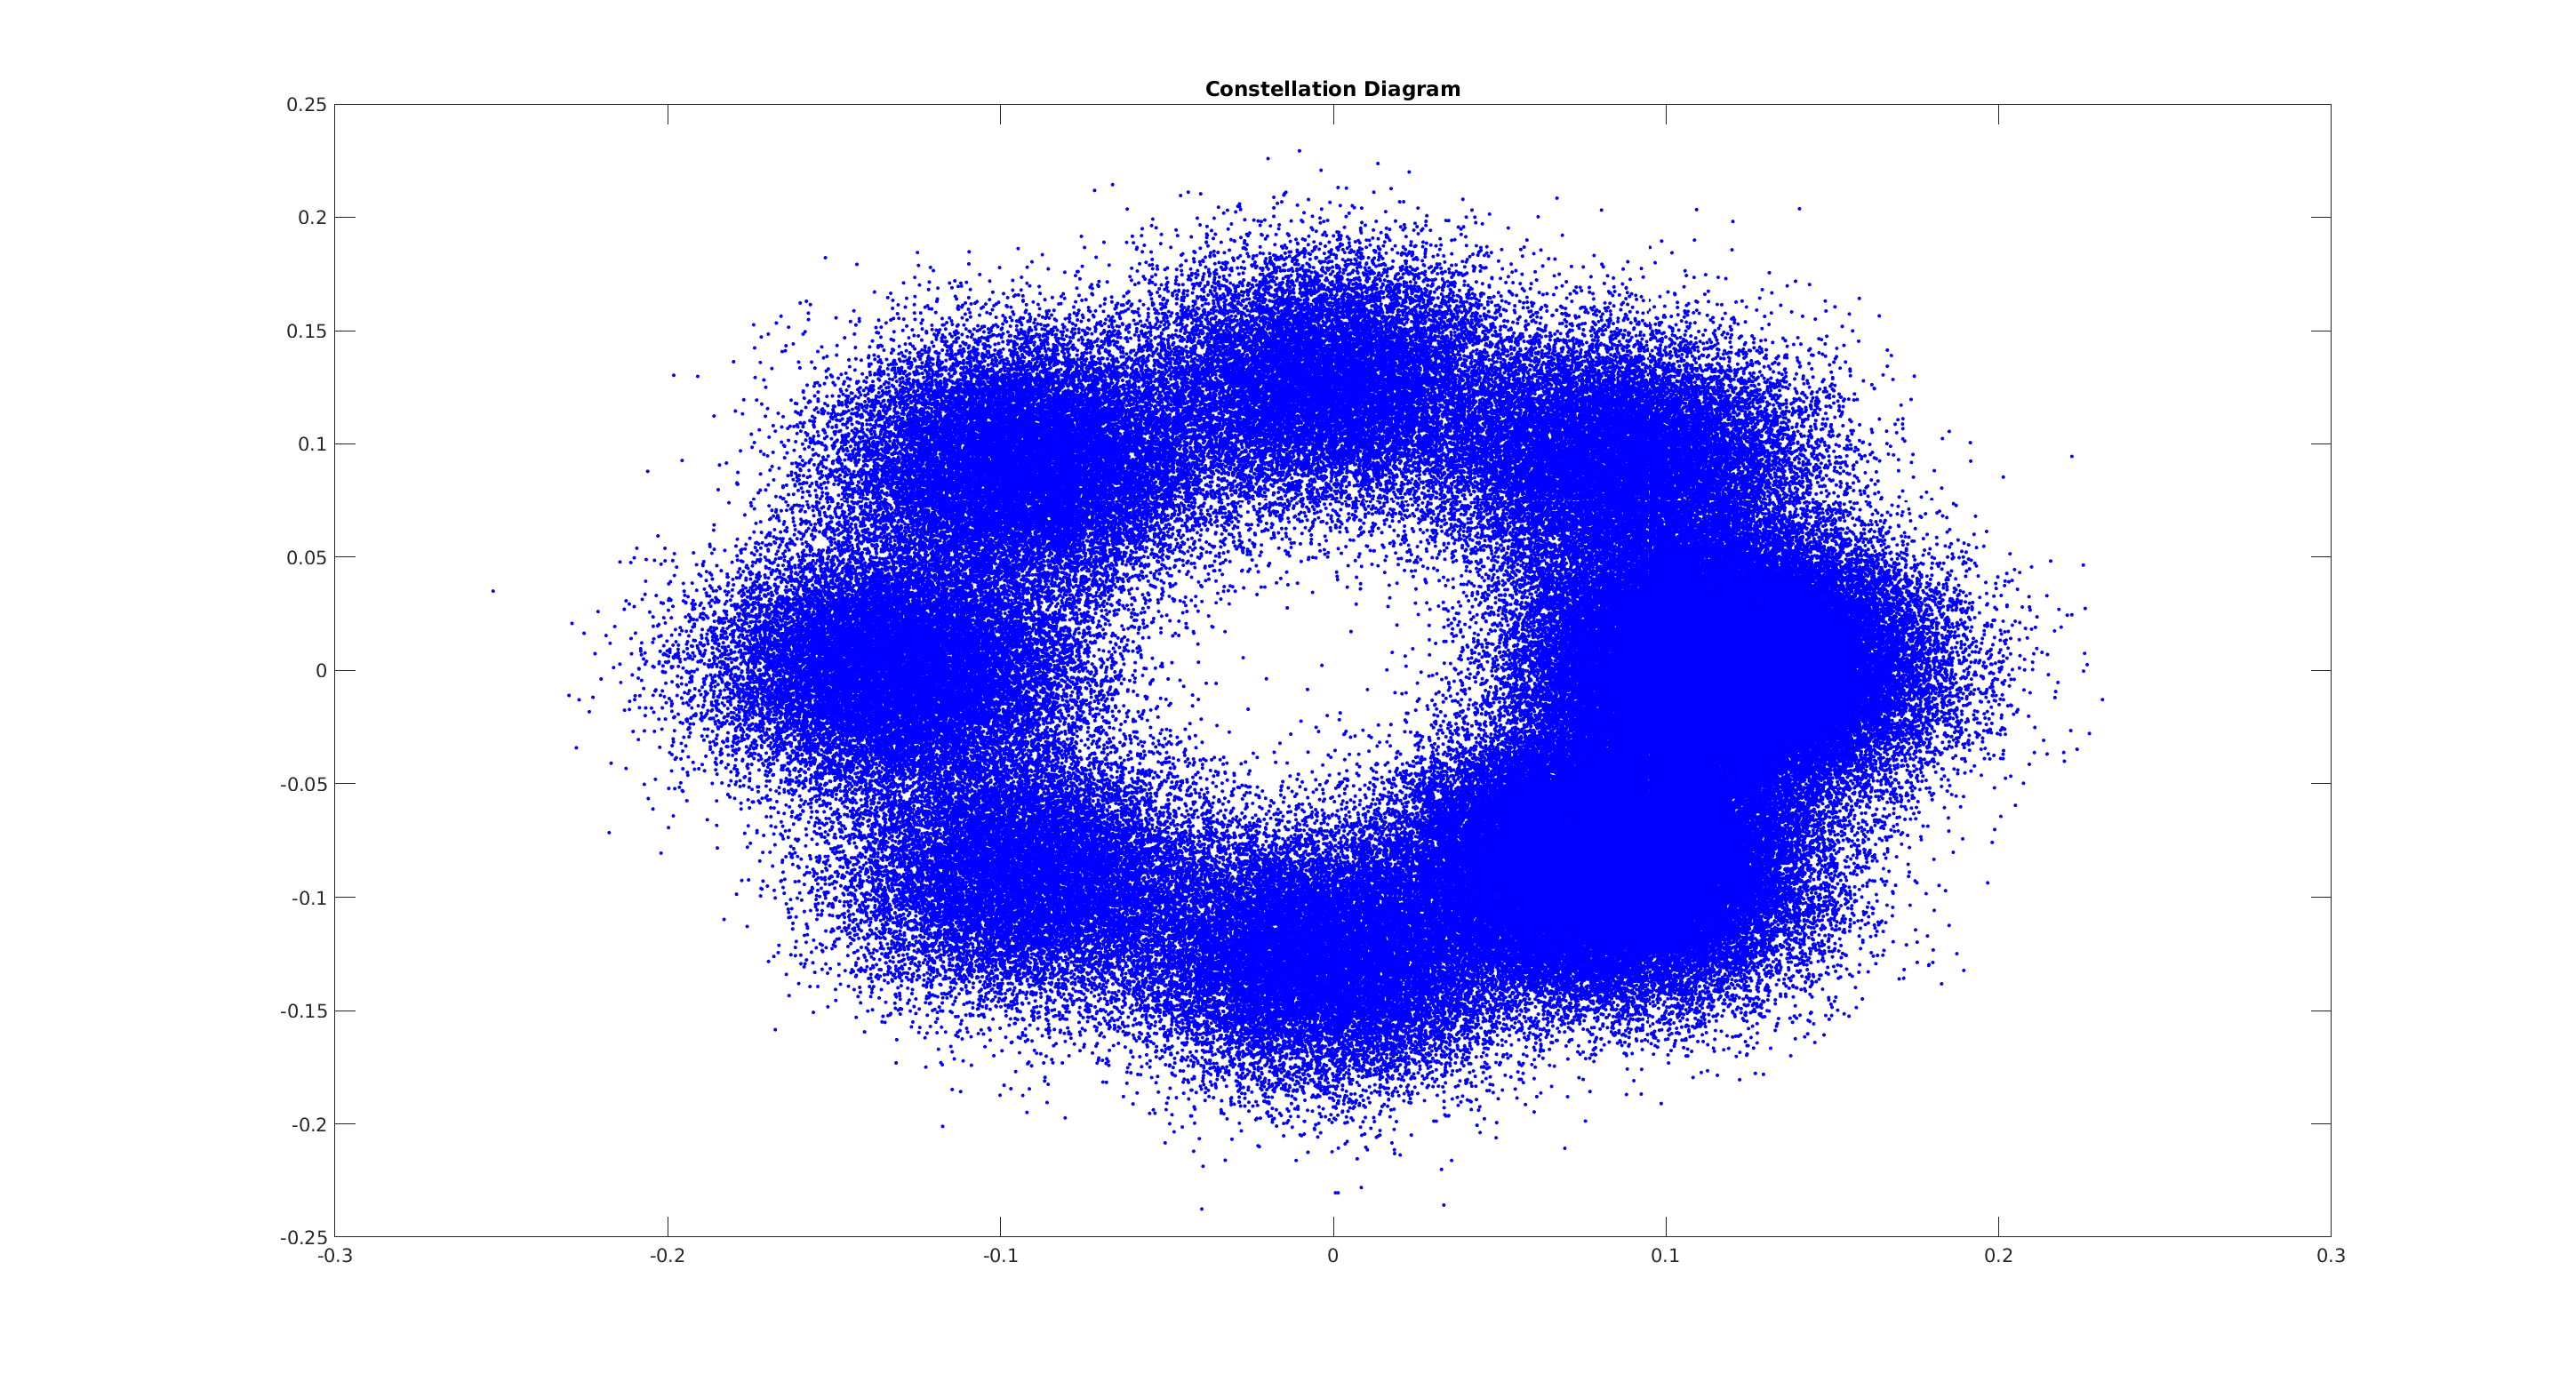
\includegraphics[width=0.9\columnwidth]{constellation8.png}
\caption{SNR=2dB}
\end{minipage}
\end{figure}


\begin{figure}[H]
\begin{minipage}[t]{0.5\linewidth}
\centering
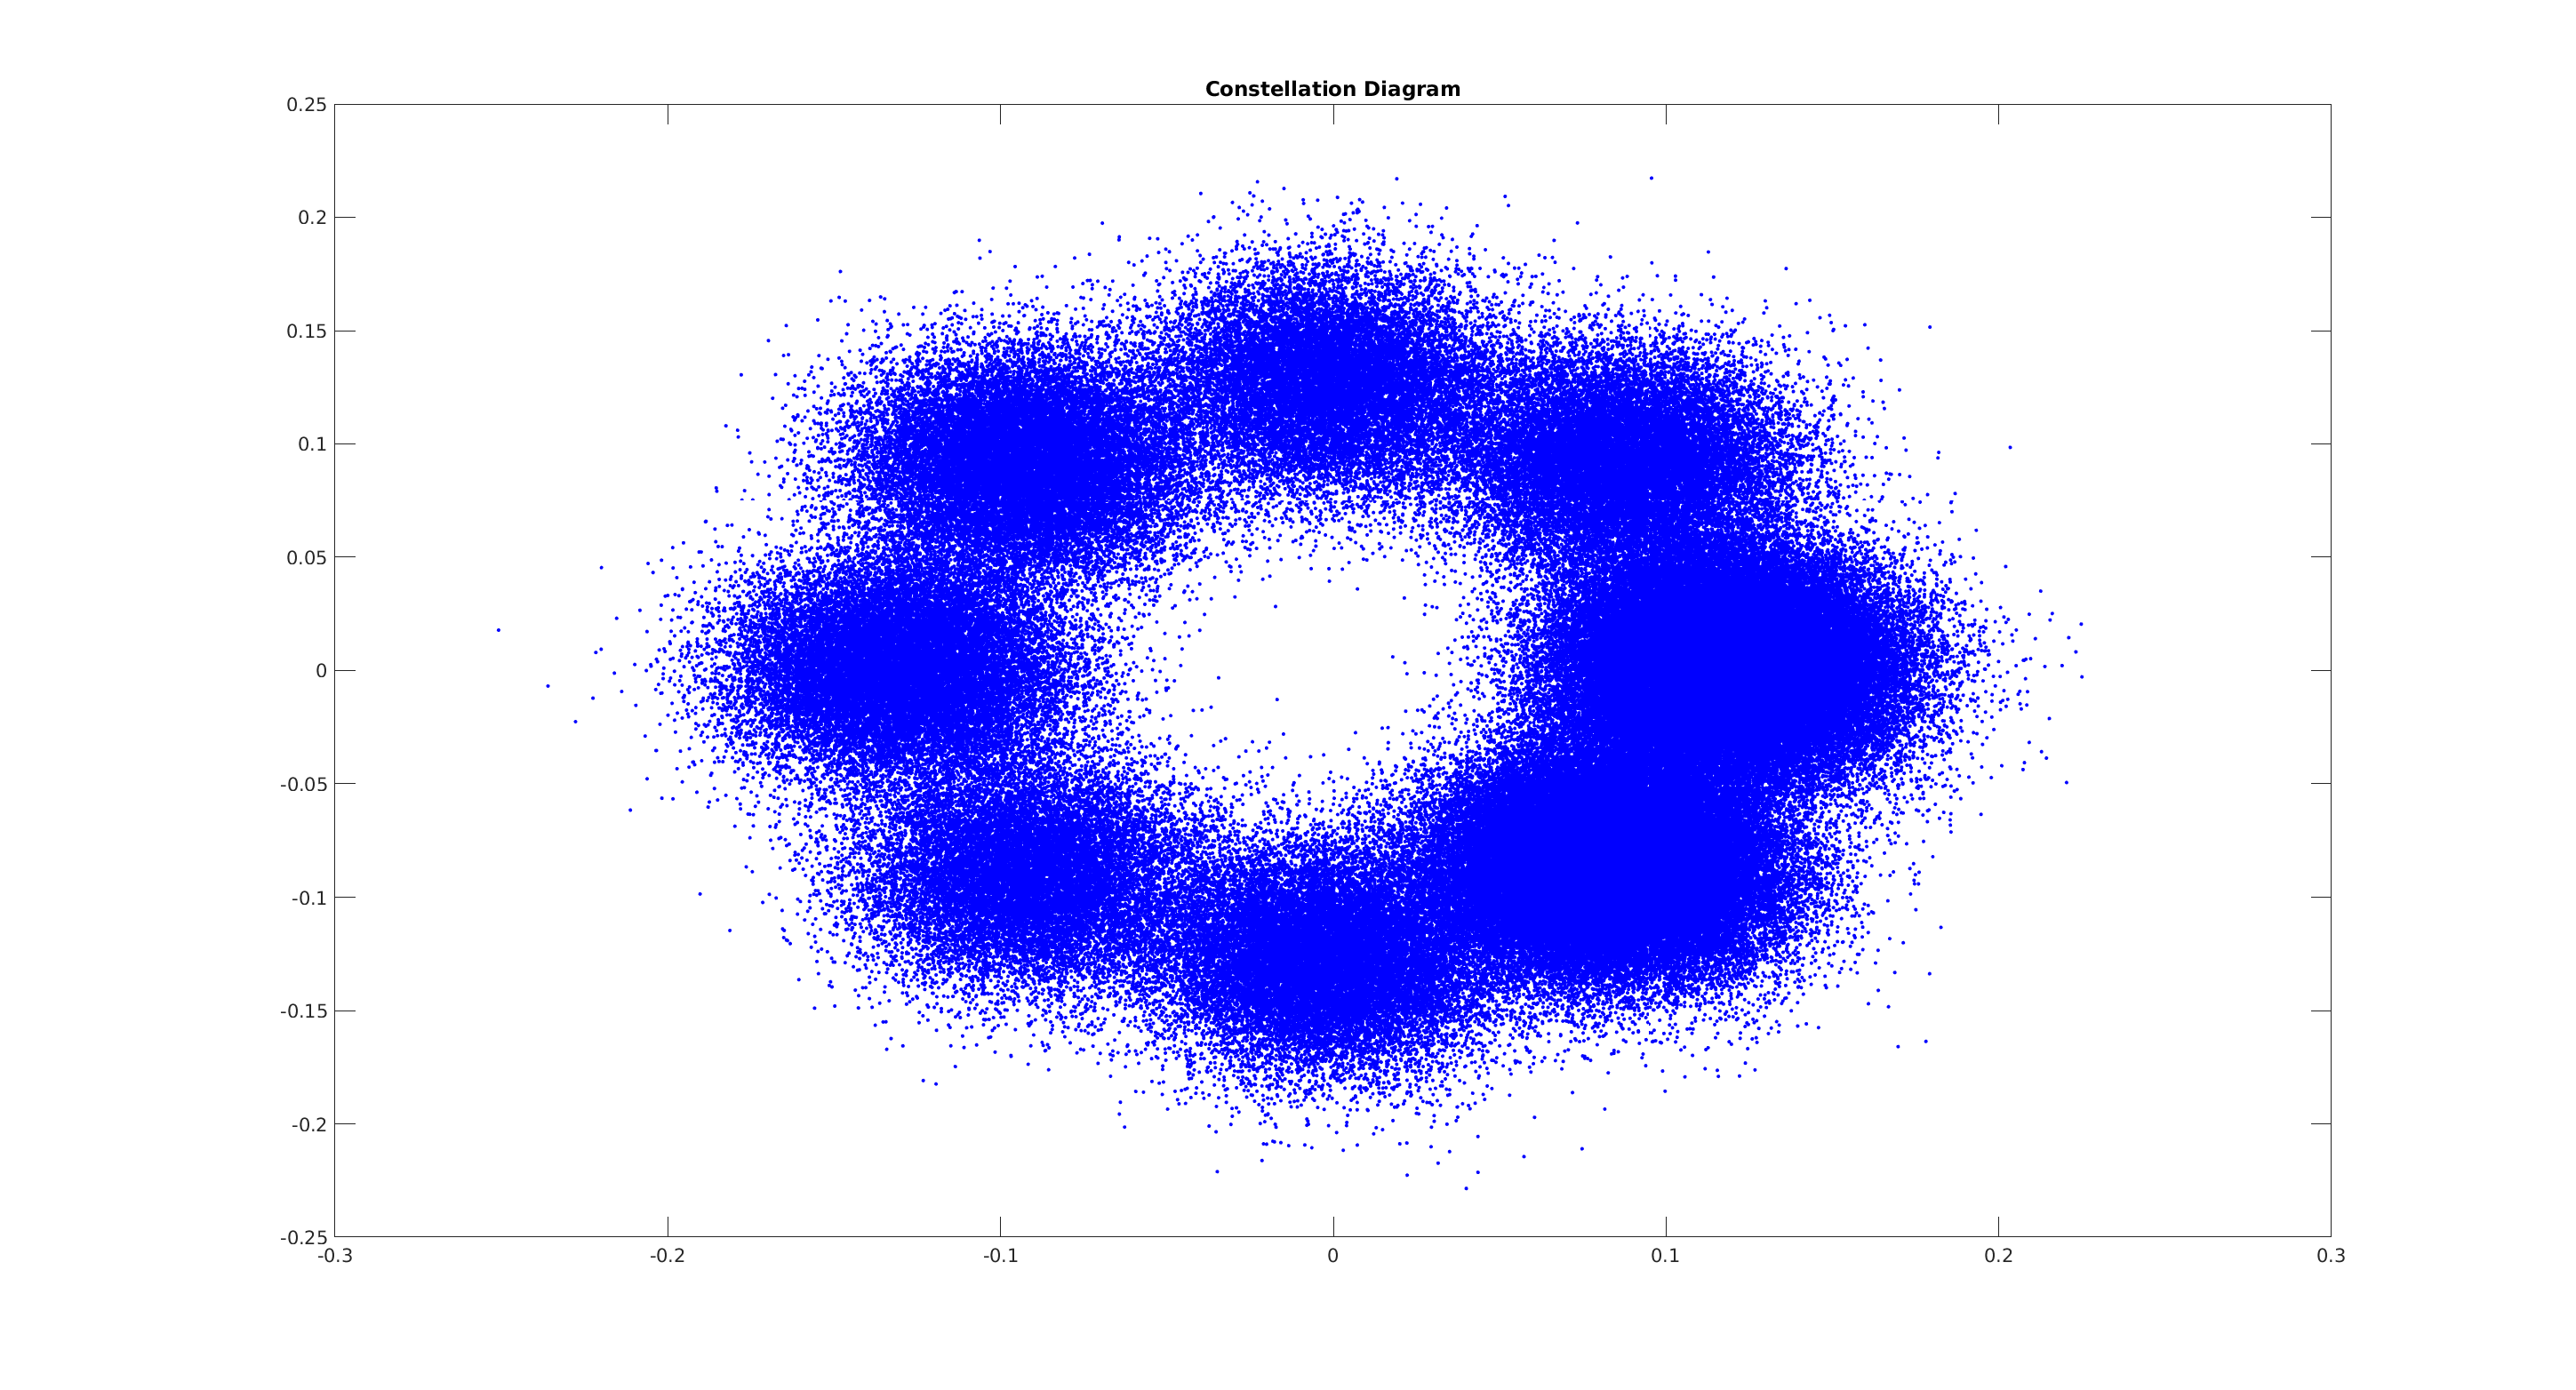
\includegraphics[width=0.9\columnwidth]{constellation9.png}
\caption{SNR=3dB}
\end{minipage}
\hfill
\begin{minipage}[t]{0.5\linewidth}
\centering
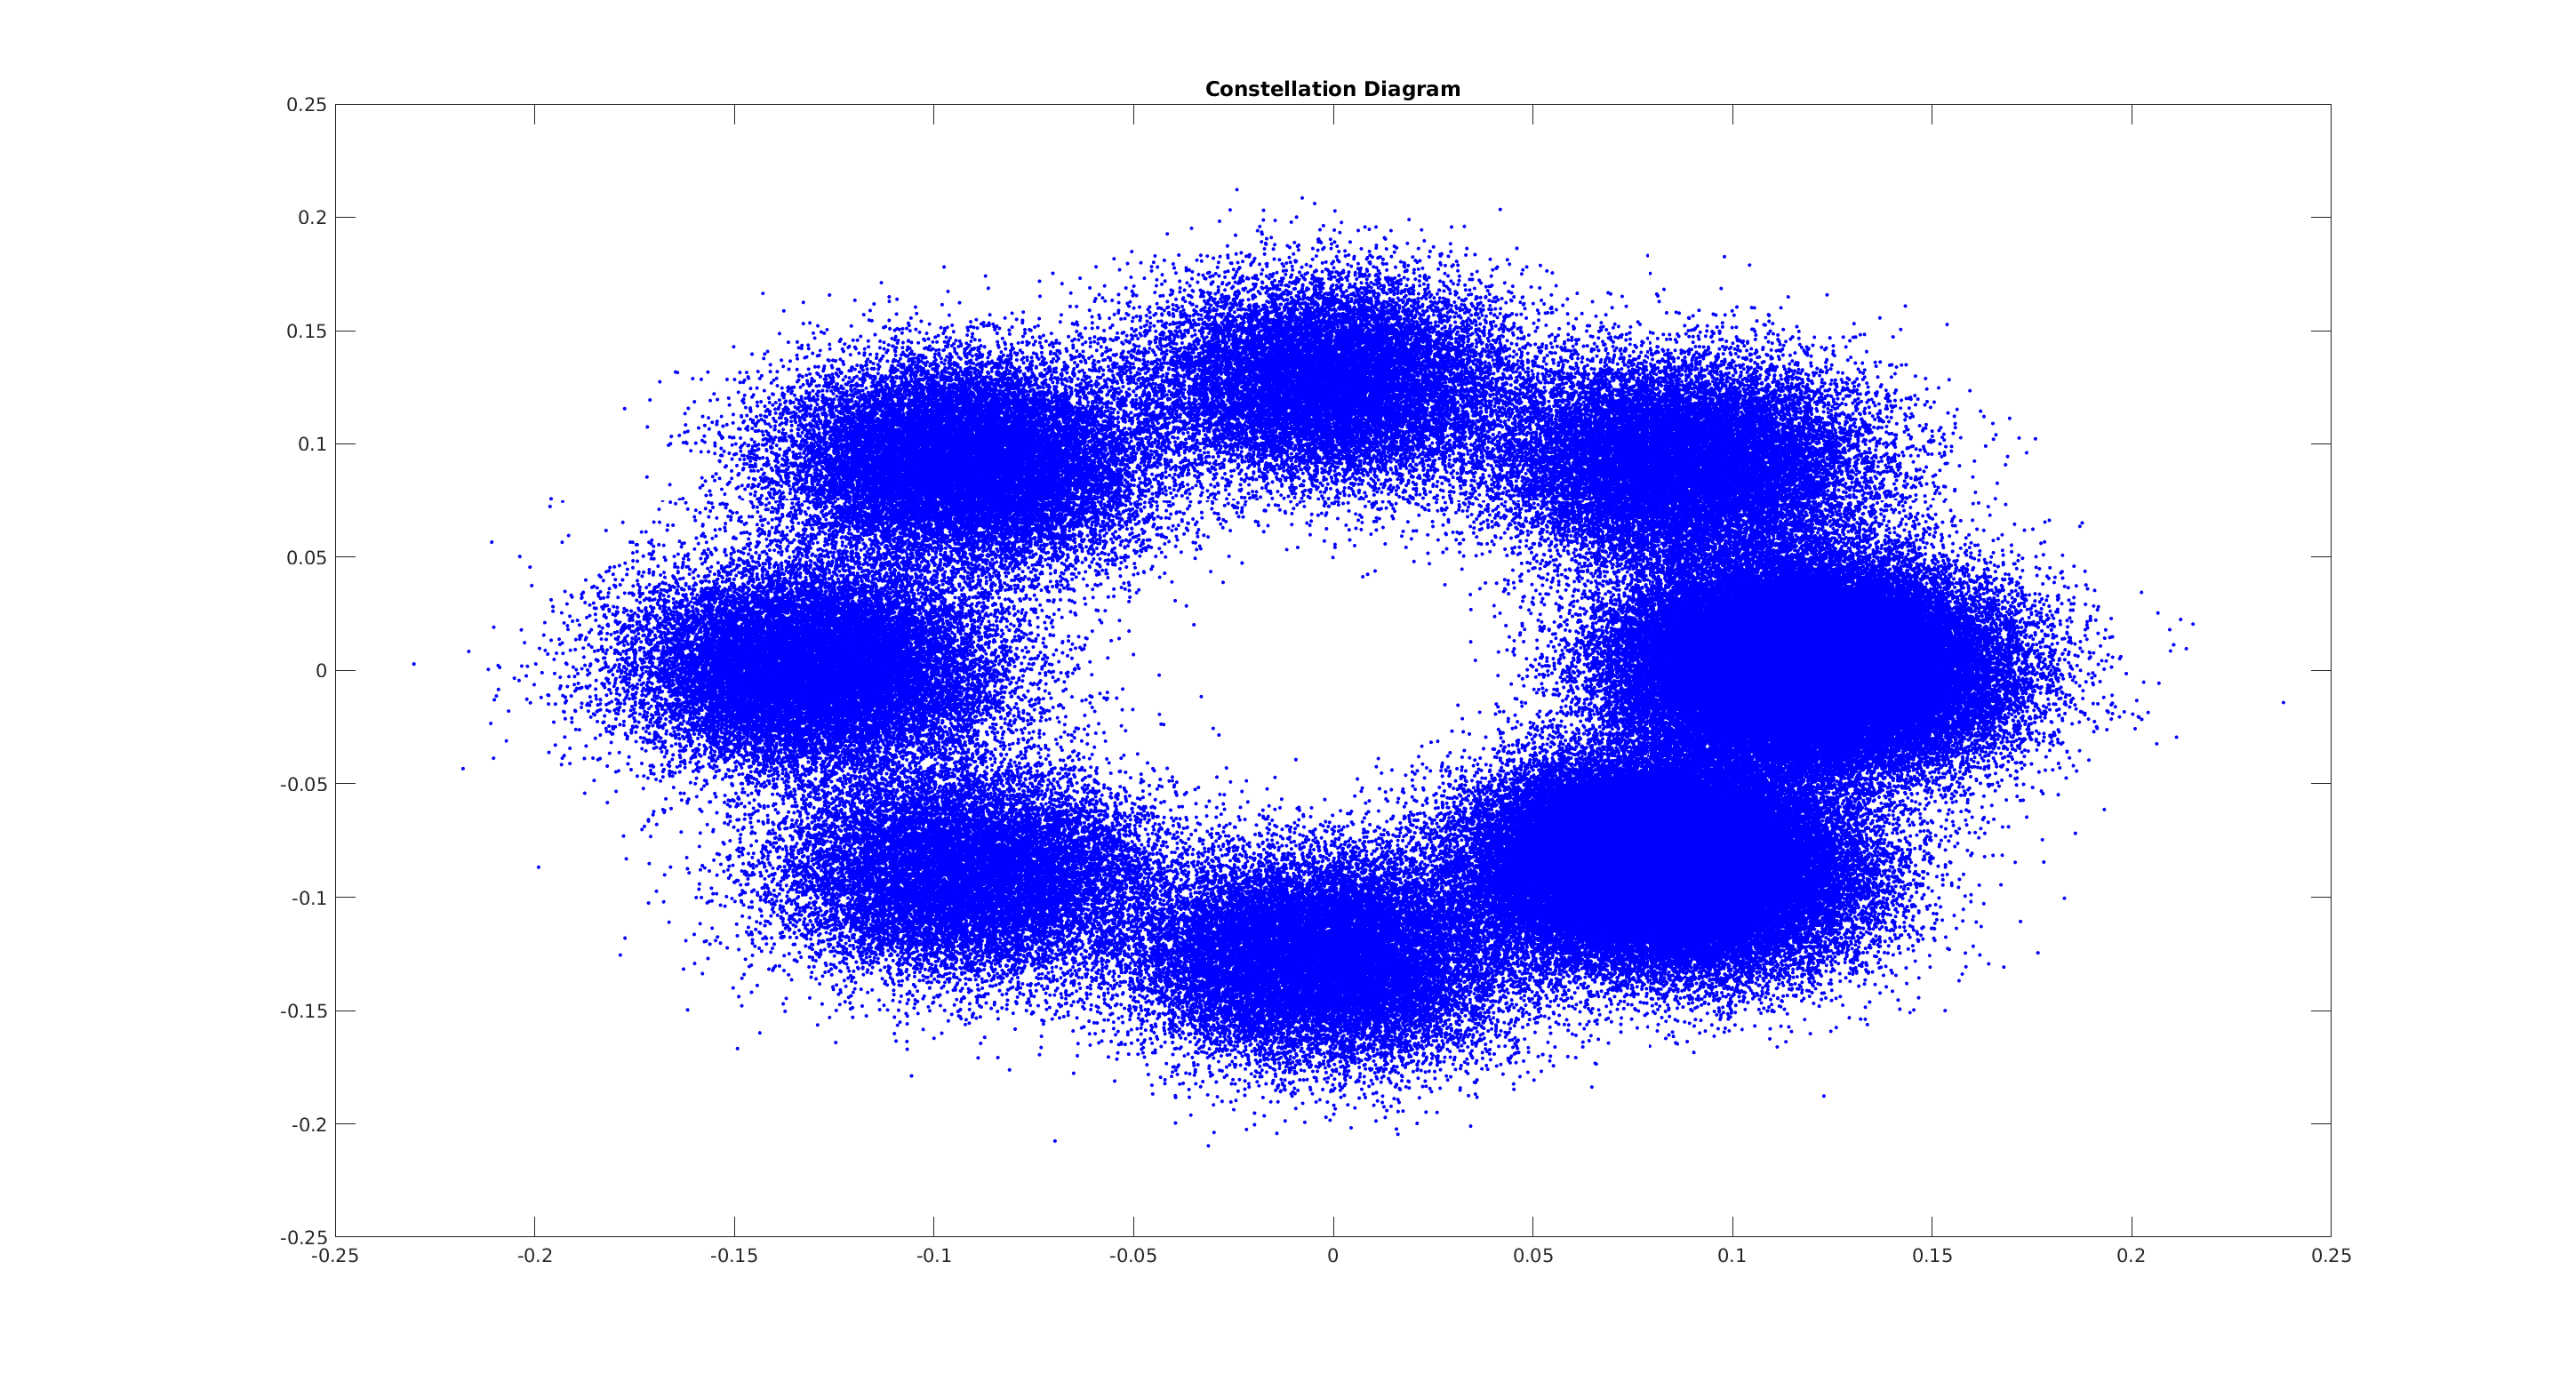
\includegraphics[width=0.9\columnwidth]{constellation10.png}
\caption{SNR=4dB}
\end{minipage}
\end{figure}


\begin{figure}[H]
\begin{minipage}[t]{0.5\linewidth}
\centering
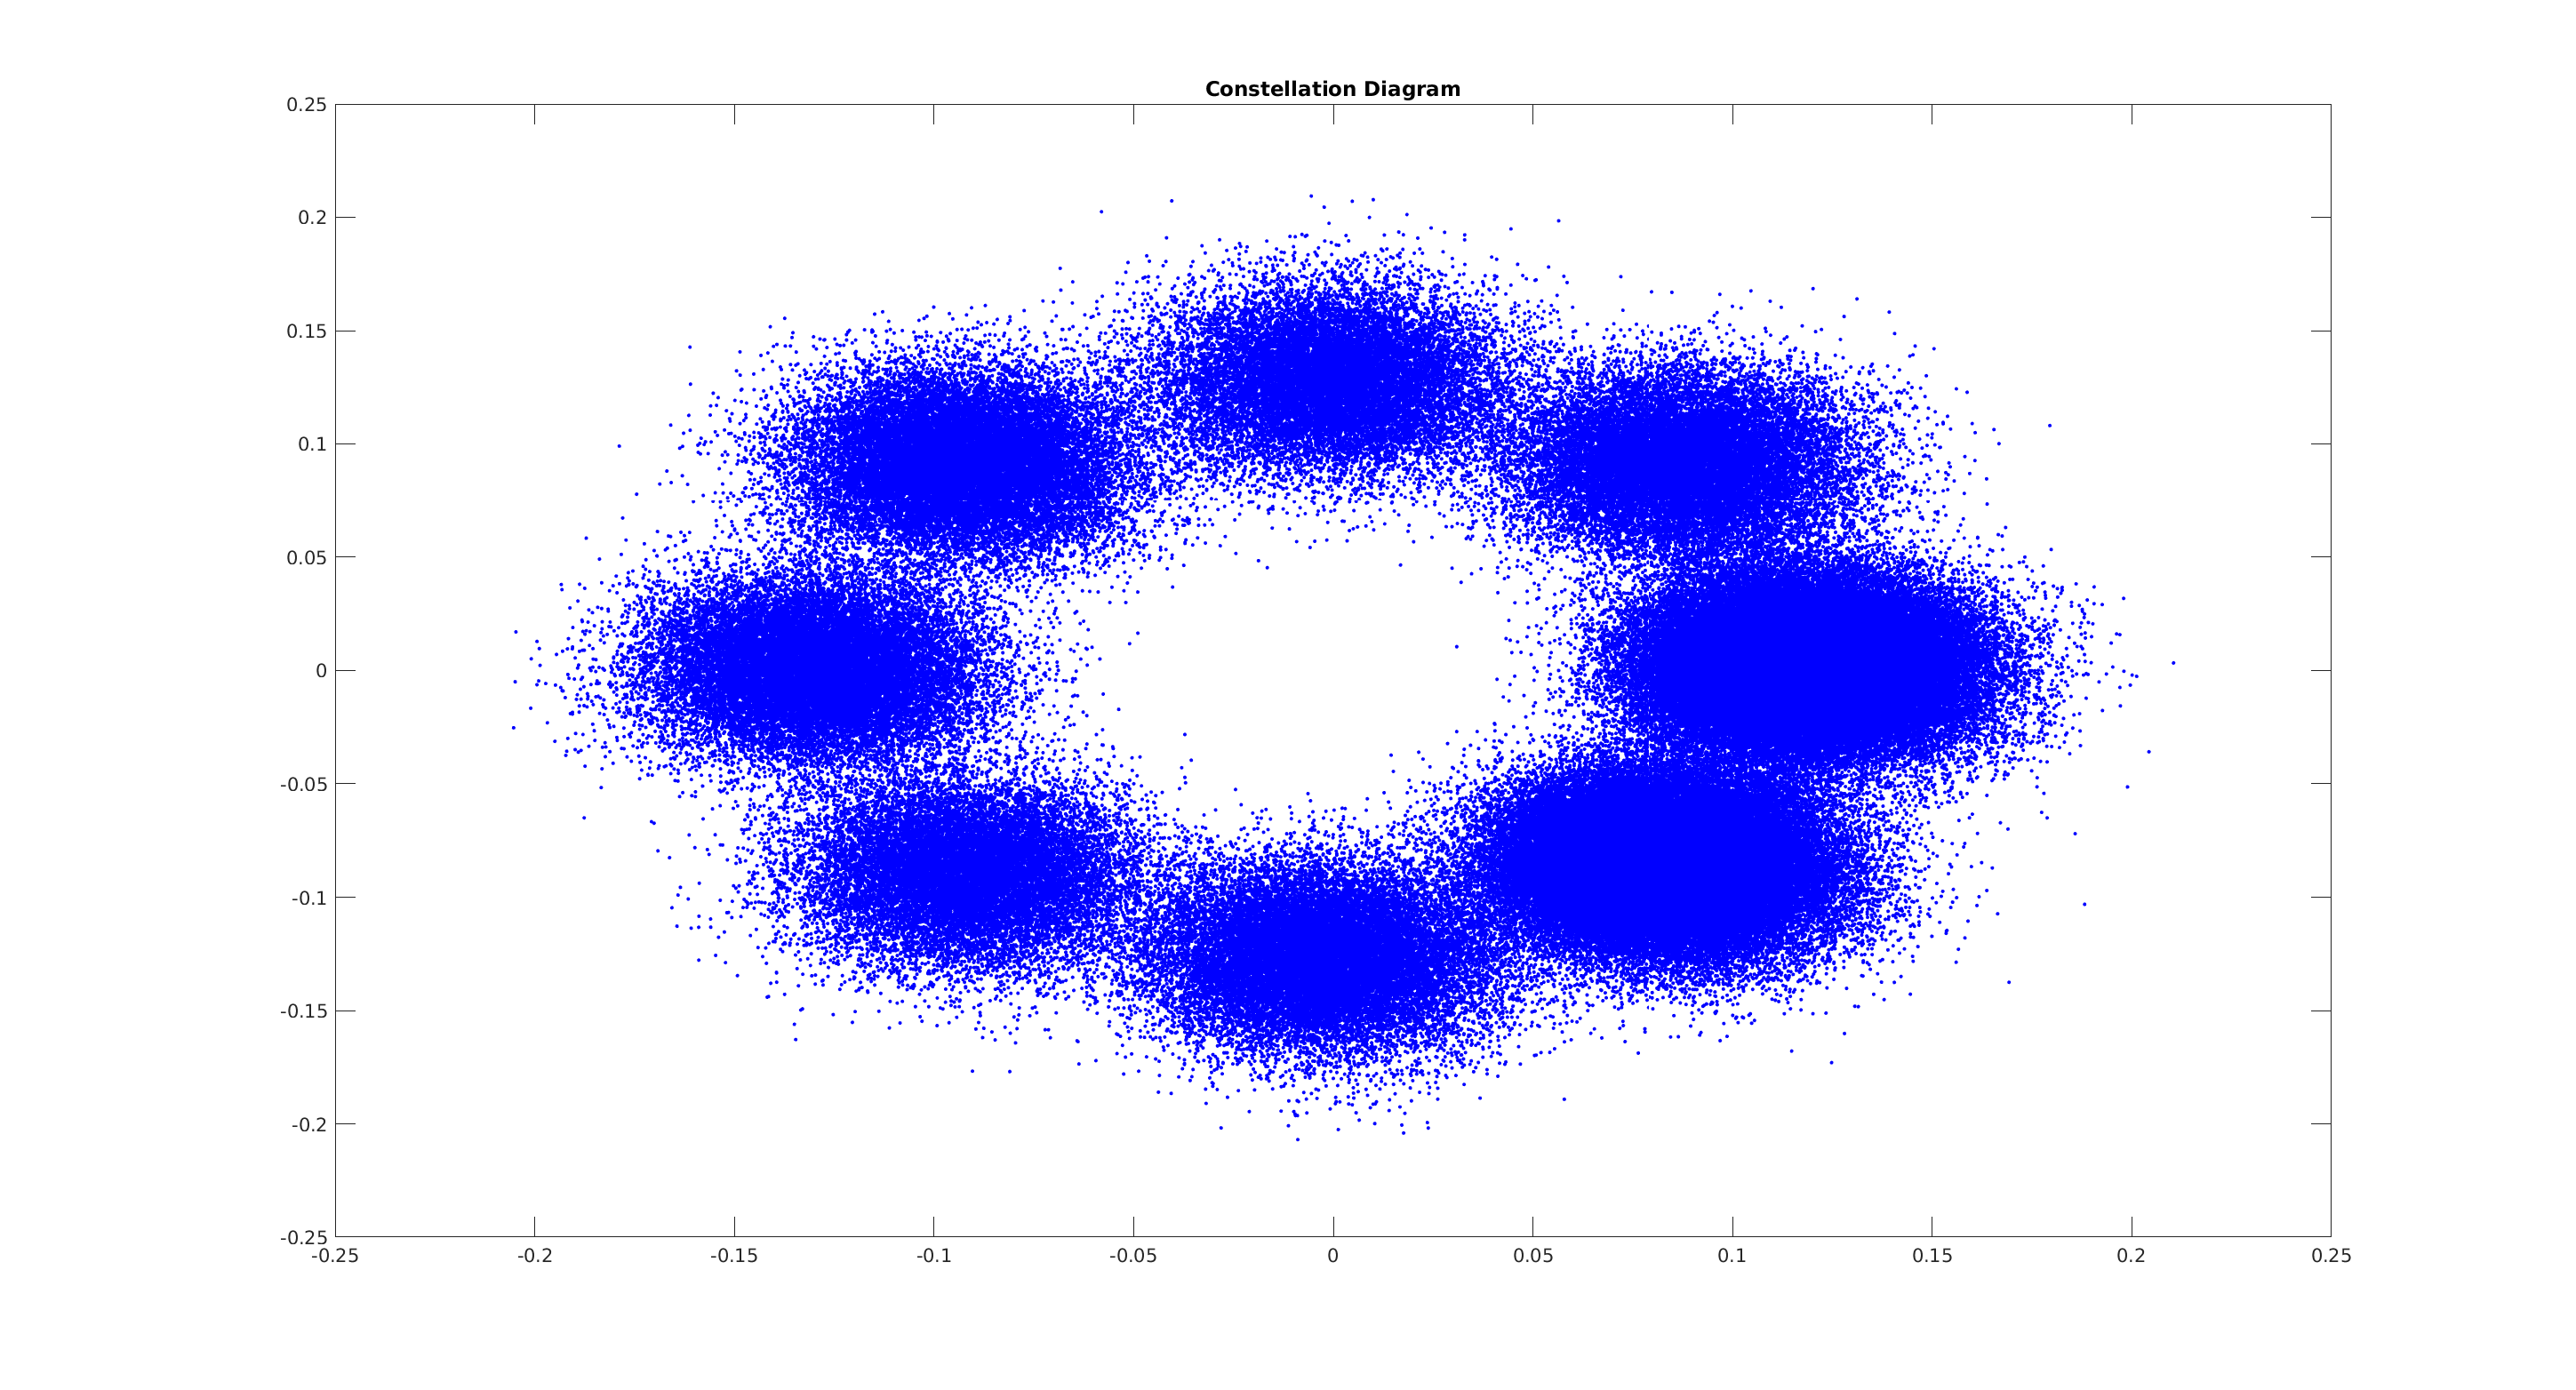
\includegraphics[width=0.9\columnwidth]{constellation11.png}
\caption{SNR=5dB}
\end{minipage}
\hfill
\begin{minipage}[t]{0.5\linewidth}
\centering
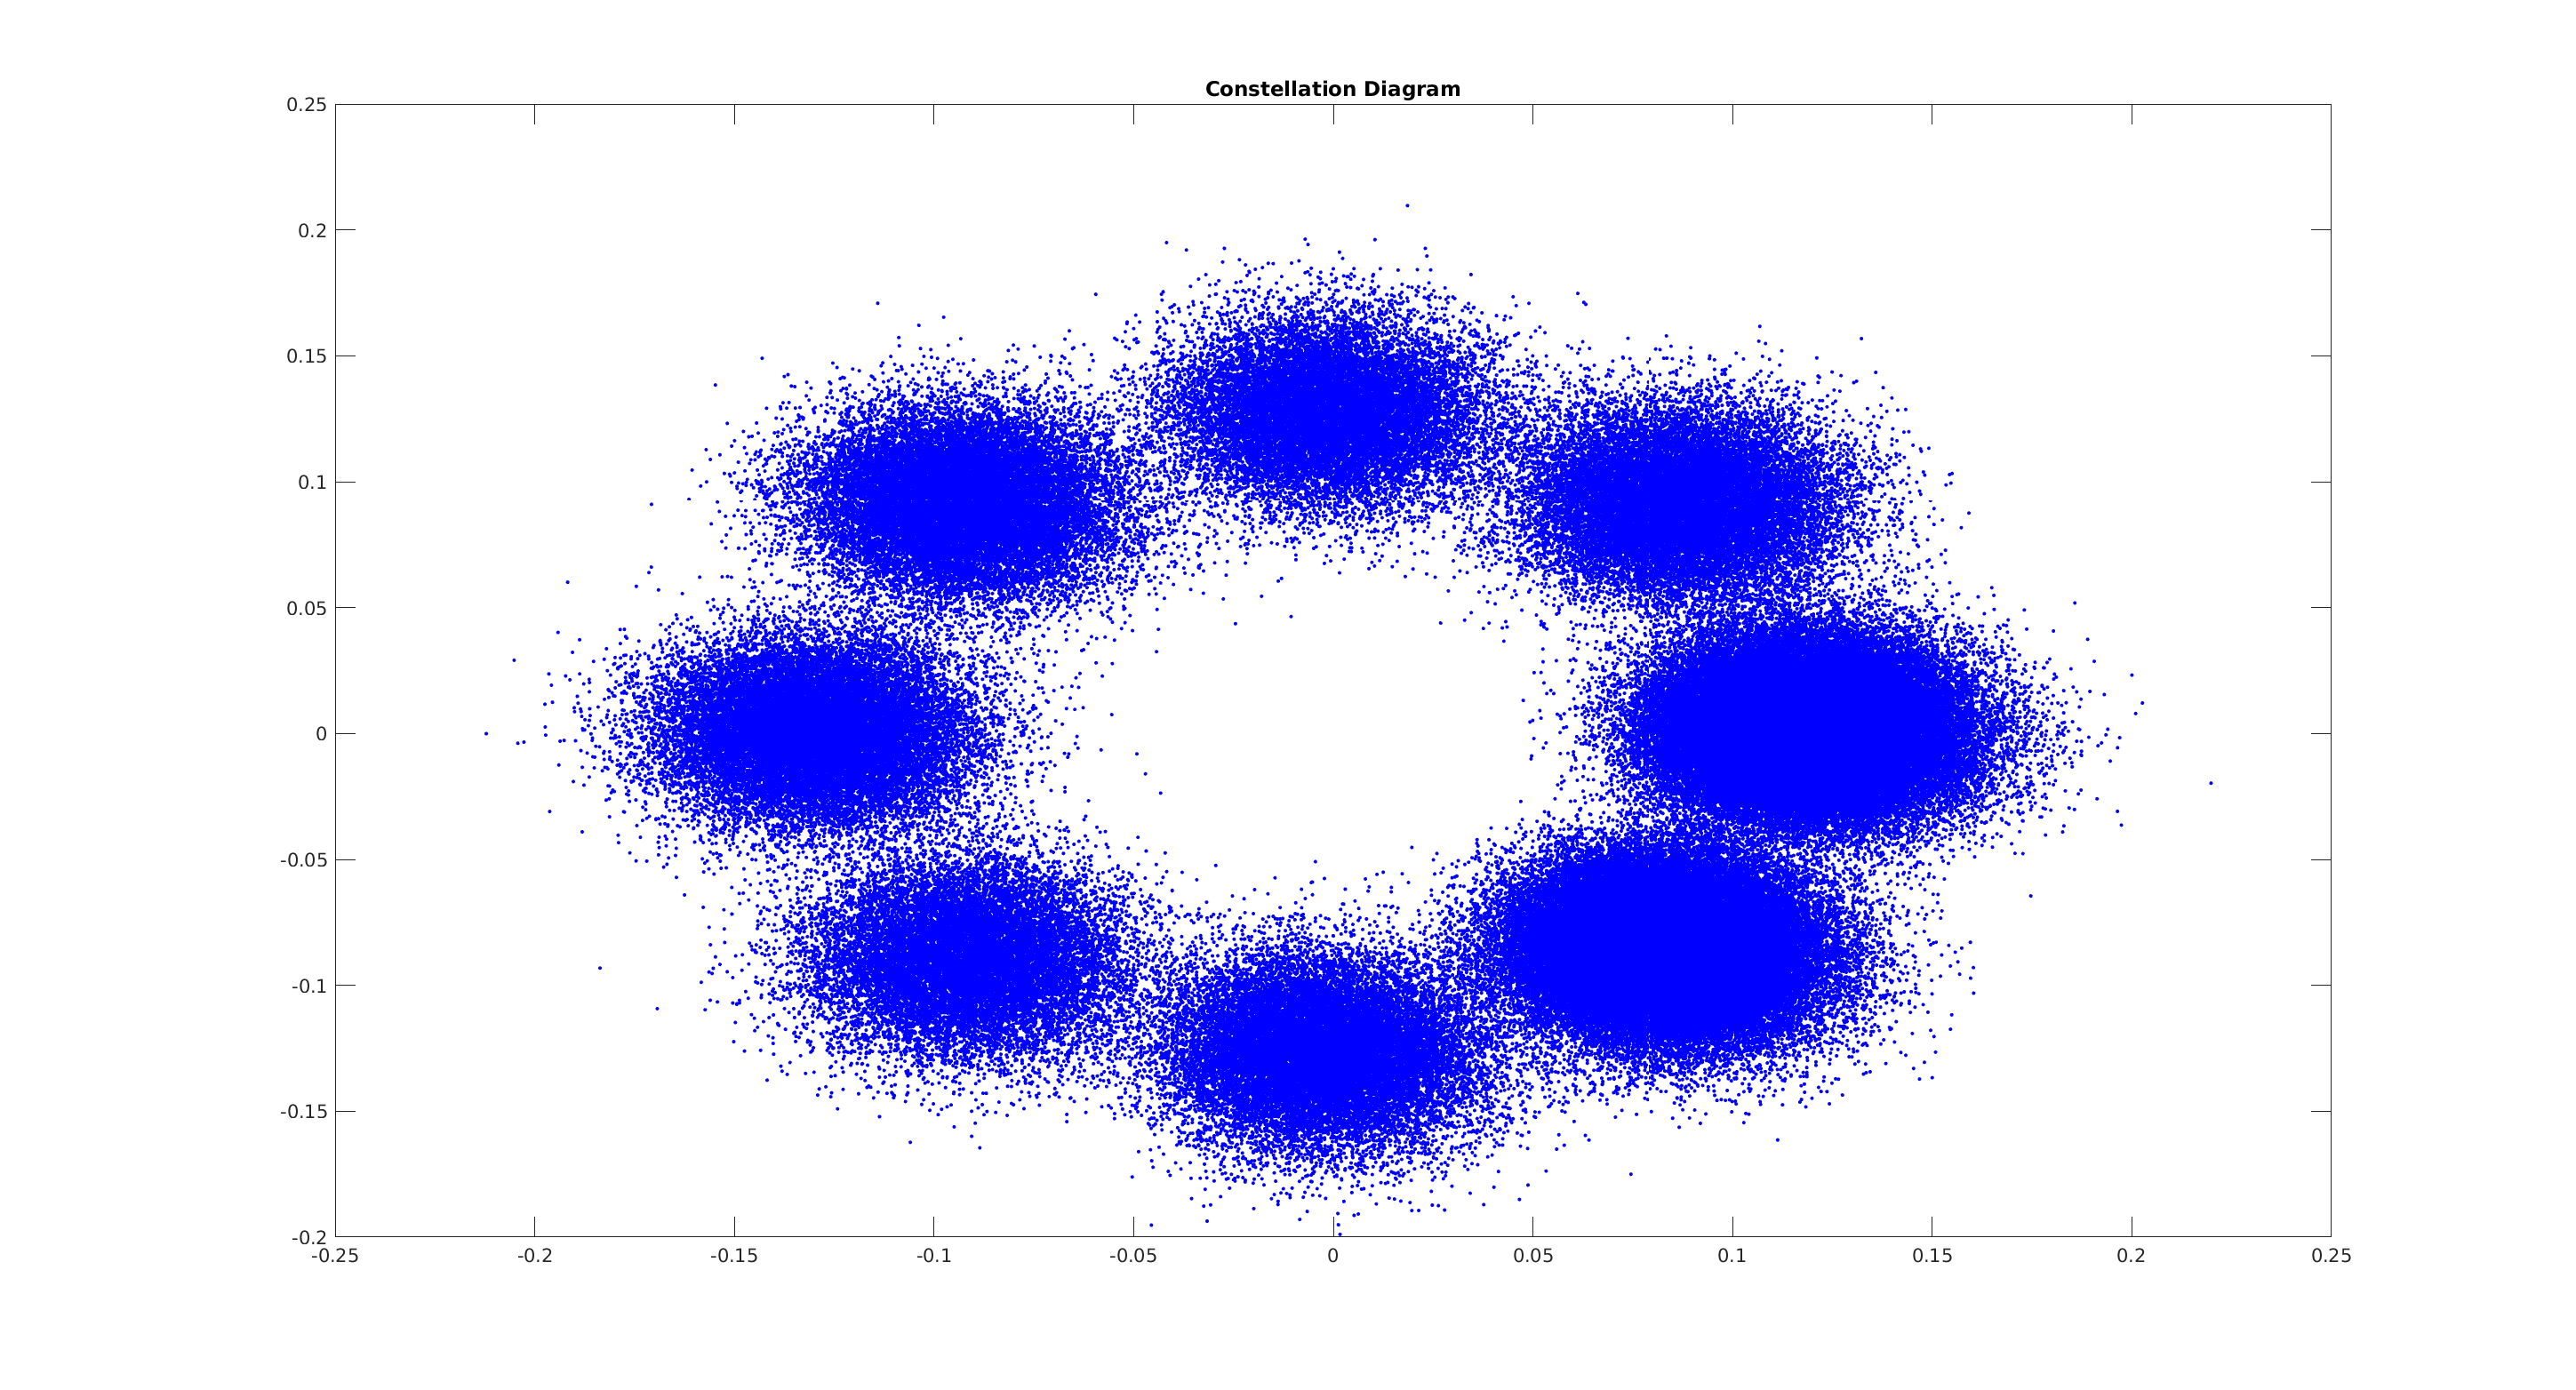
\includegraphics[width=0.9\columnwidth]{constellation12.png}
\caption{SNR=6dB}
\end{minipage}
\end{figure}


\begin{figure}[H]
\begin{minipage}[t]{0.5\linewidth}
\centering
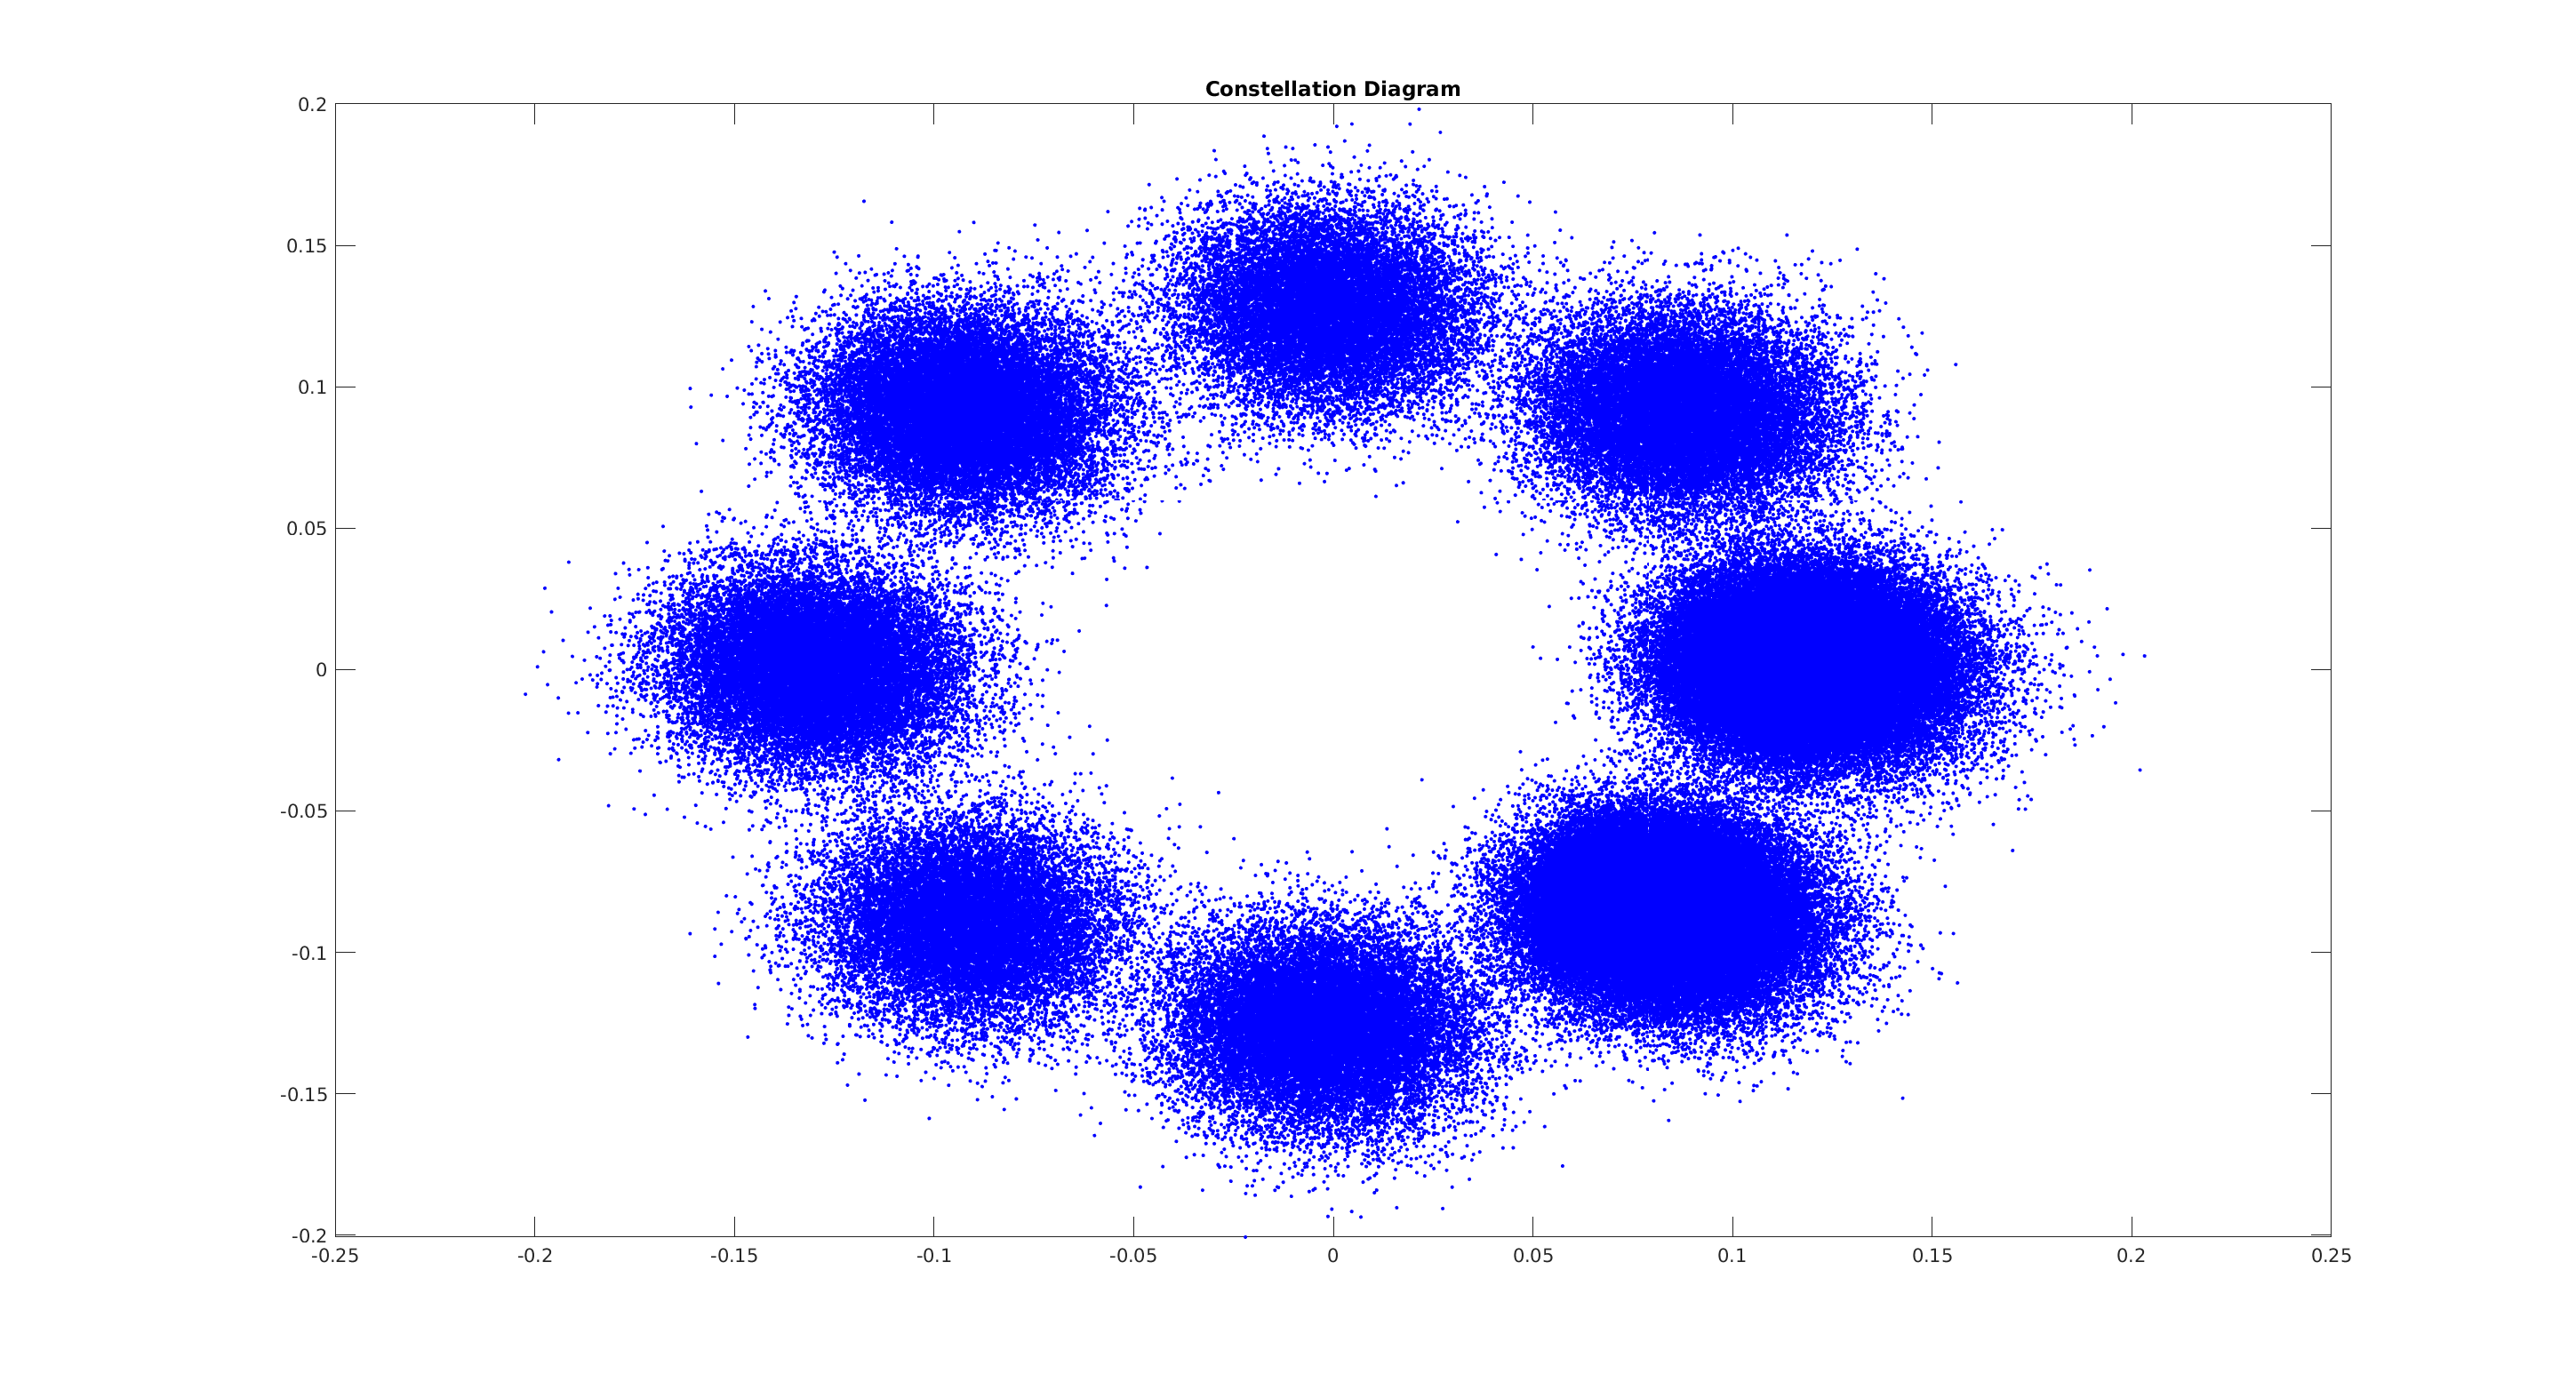
\includegraphics[width=0.9\columnwidth]{constellation13.png}
\caption{SNR=7dB}
\end{minipage}
\hfill
\begin{minipage}[t]{0.5\linewidth}
\centering
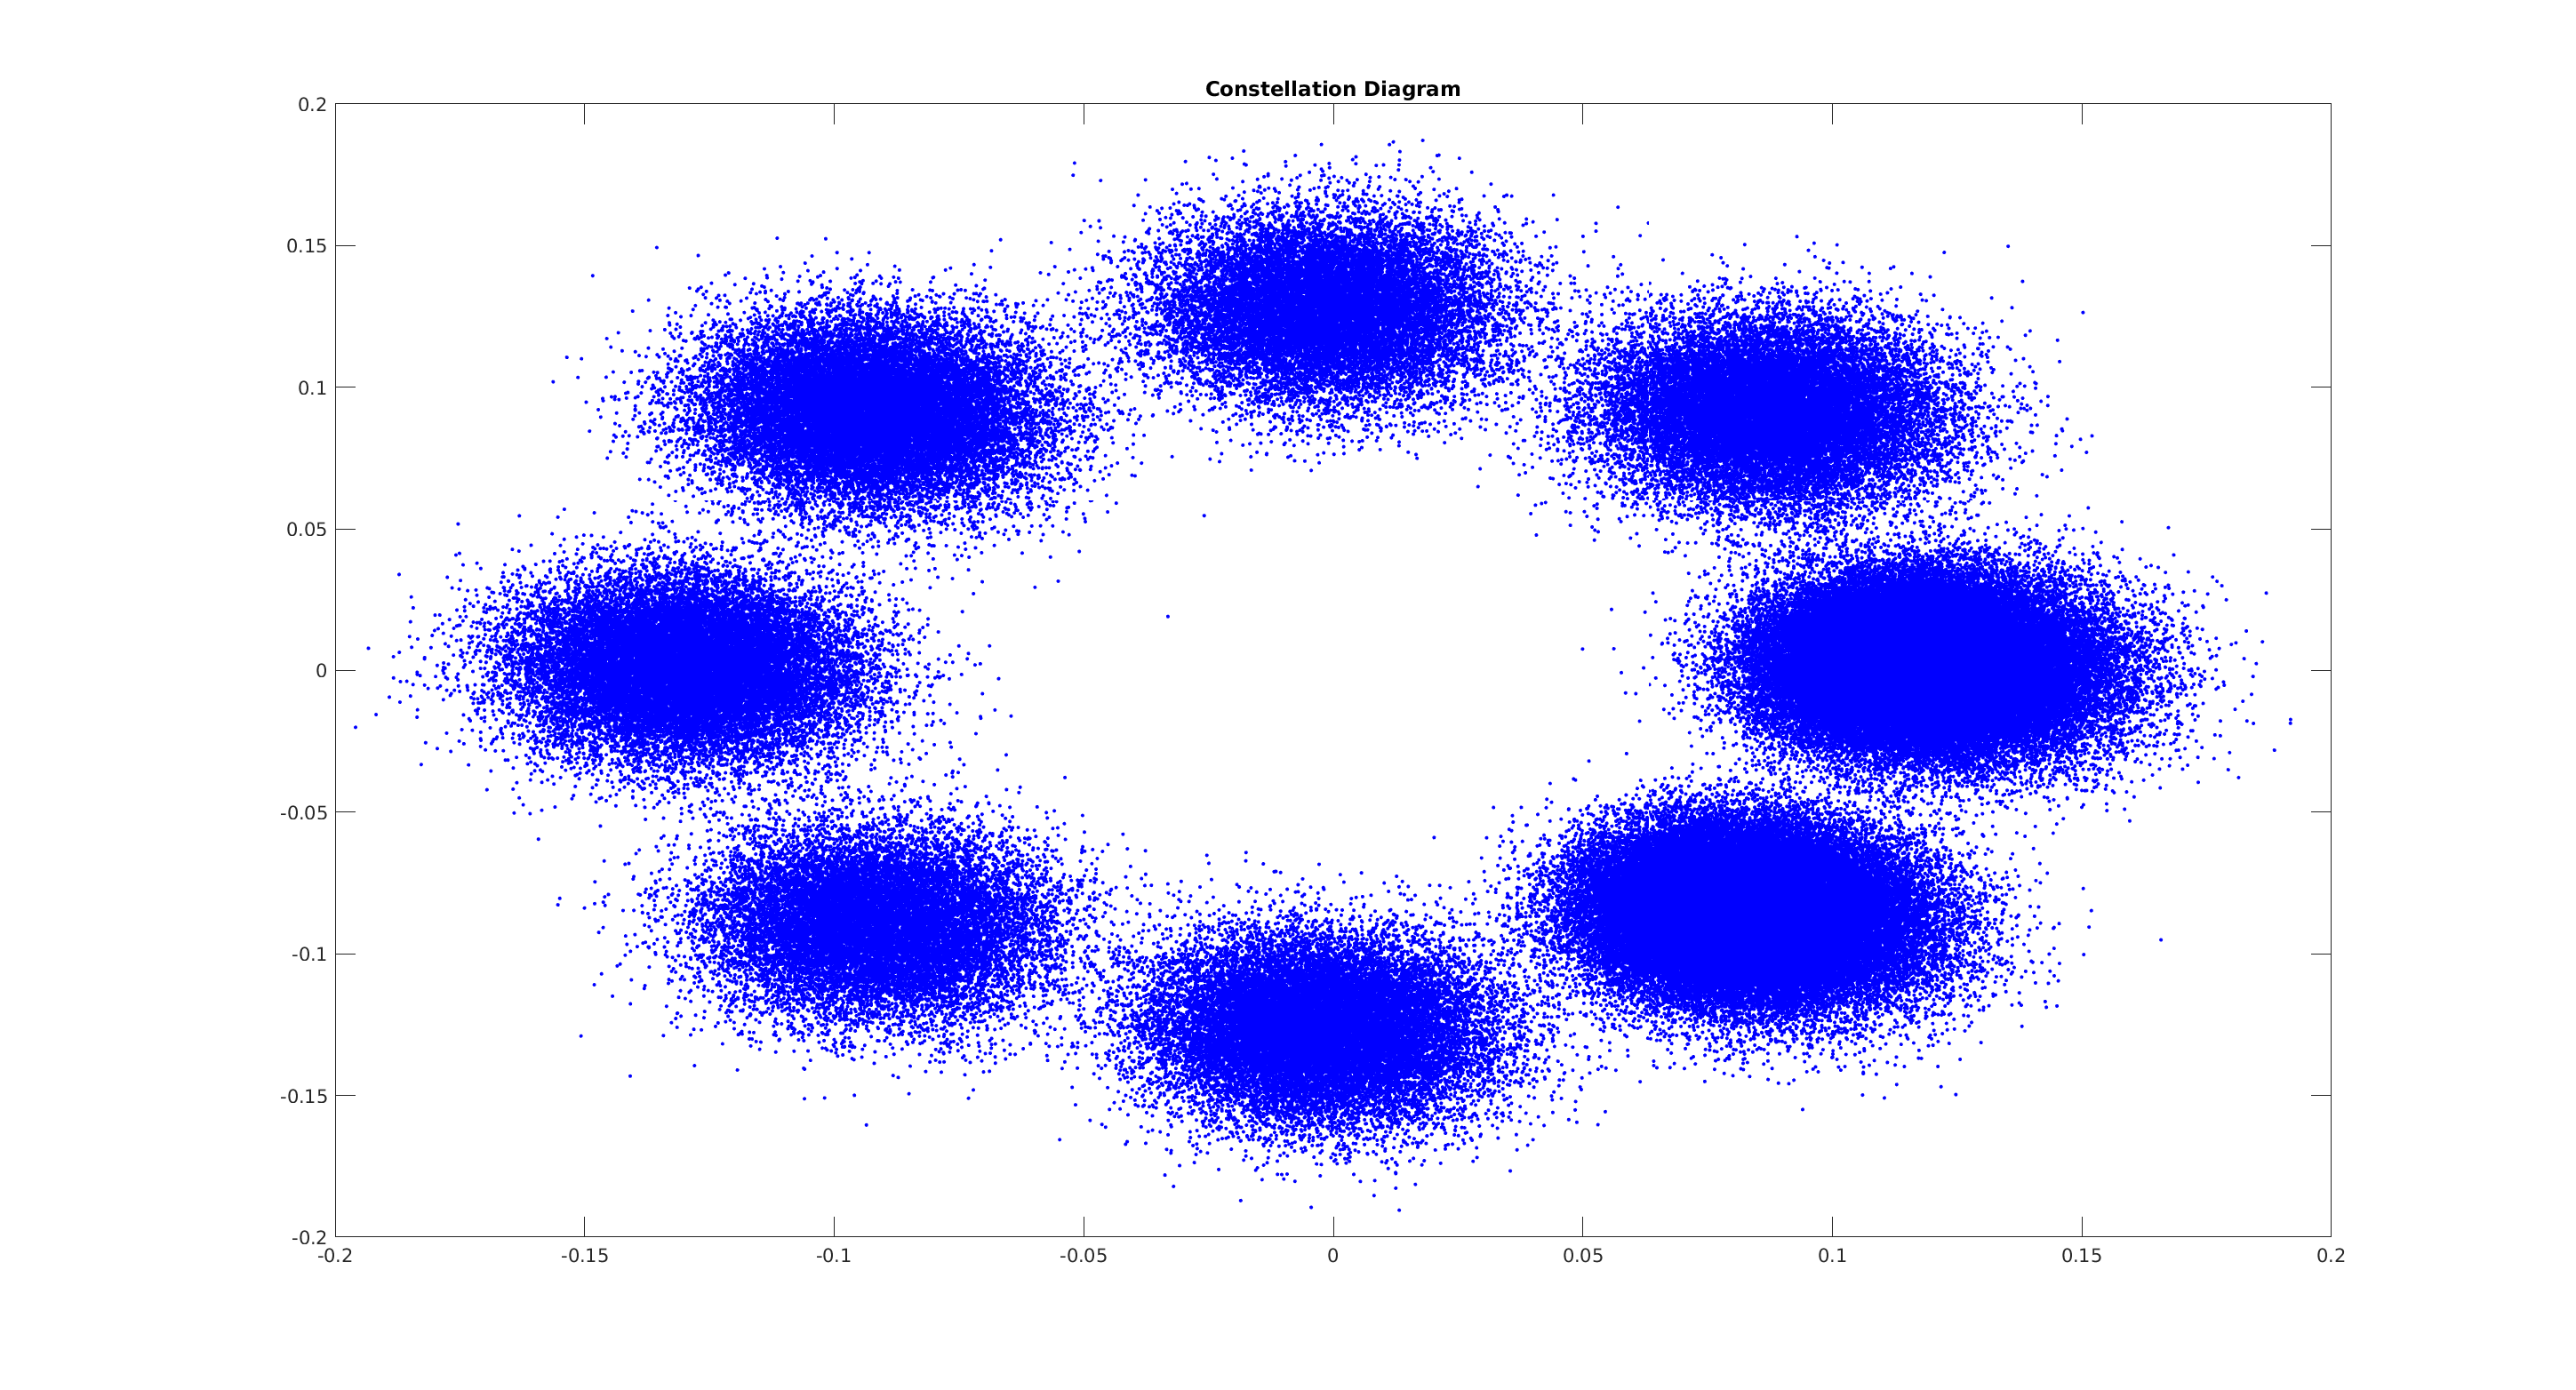
\includegraphics[width=0.9\columnwidth]{constellation14.png}
\caption{SNR=8dB}
\end{minipage}
\end{figure}



\begin{figure}[H]
\begin{minipage}[t]{0.5\linewidth}
\centering
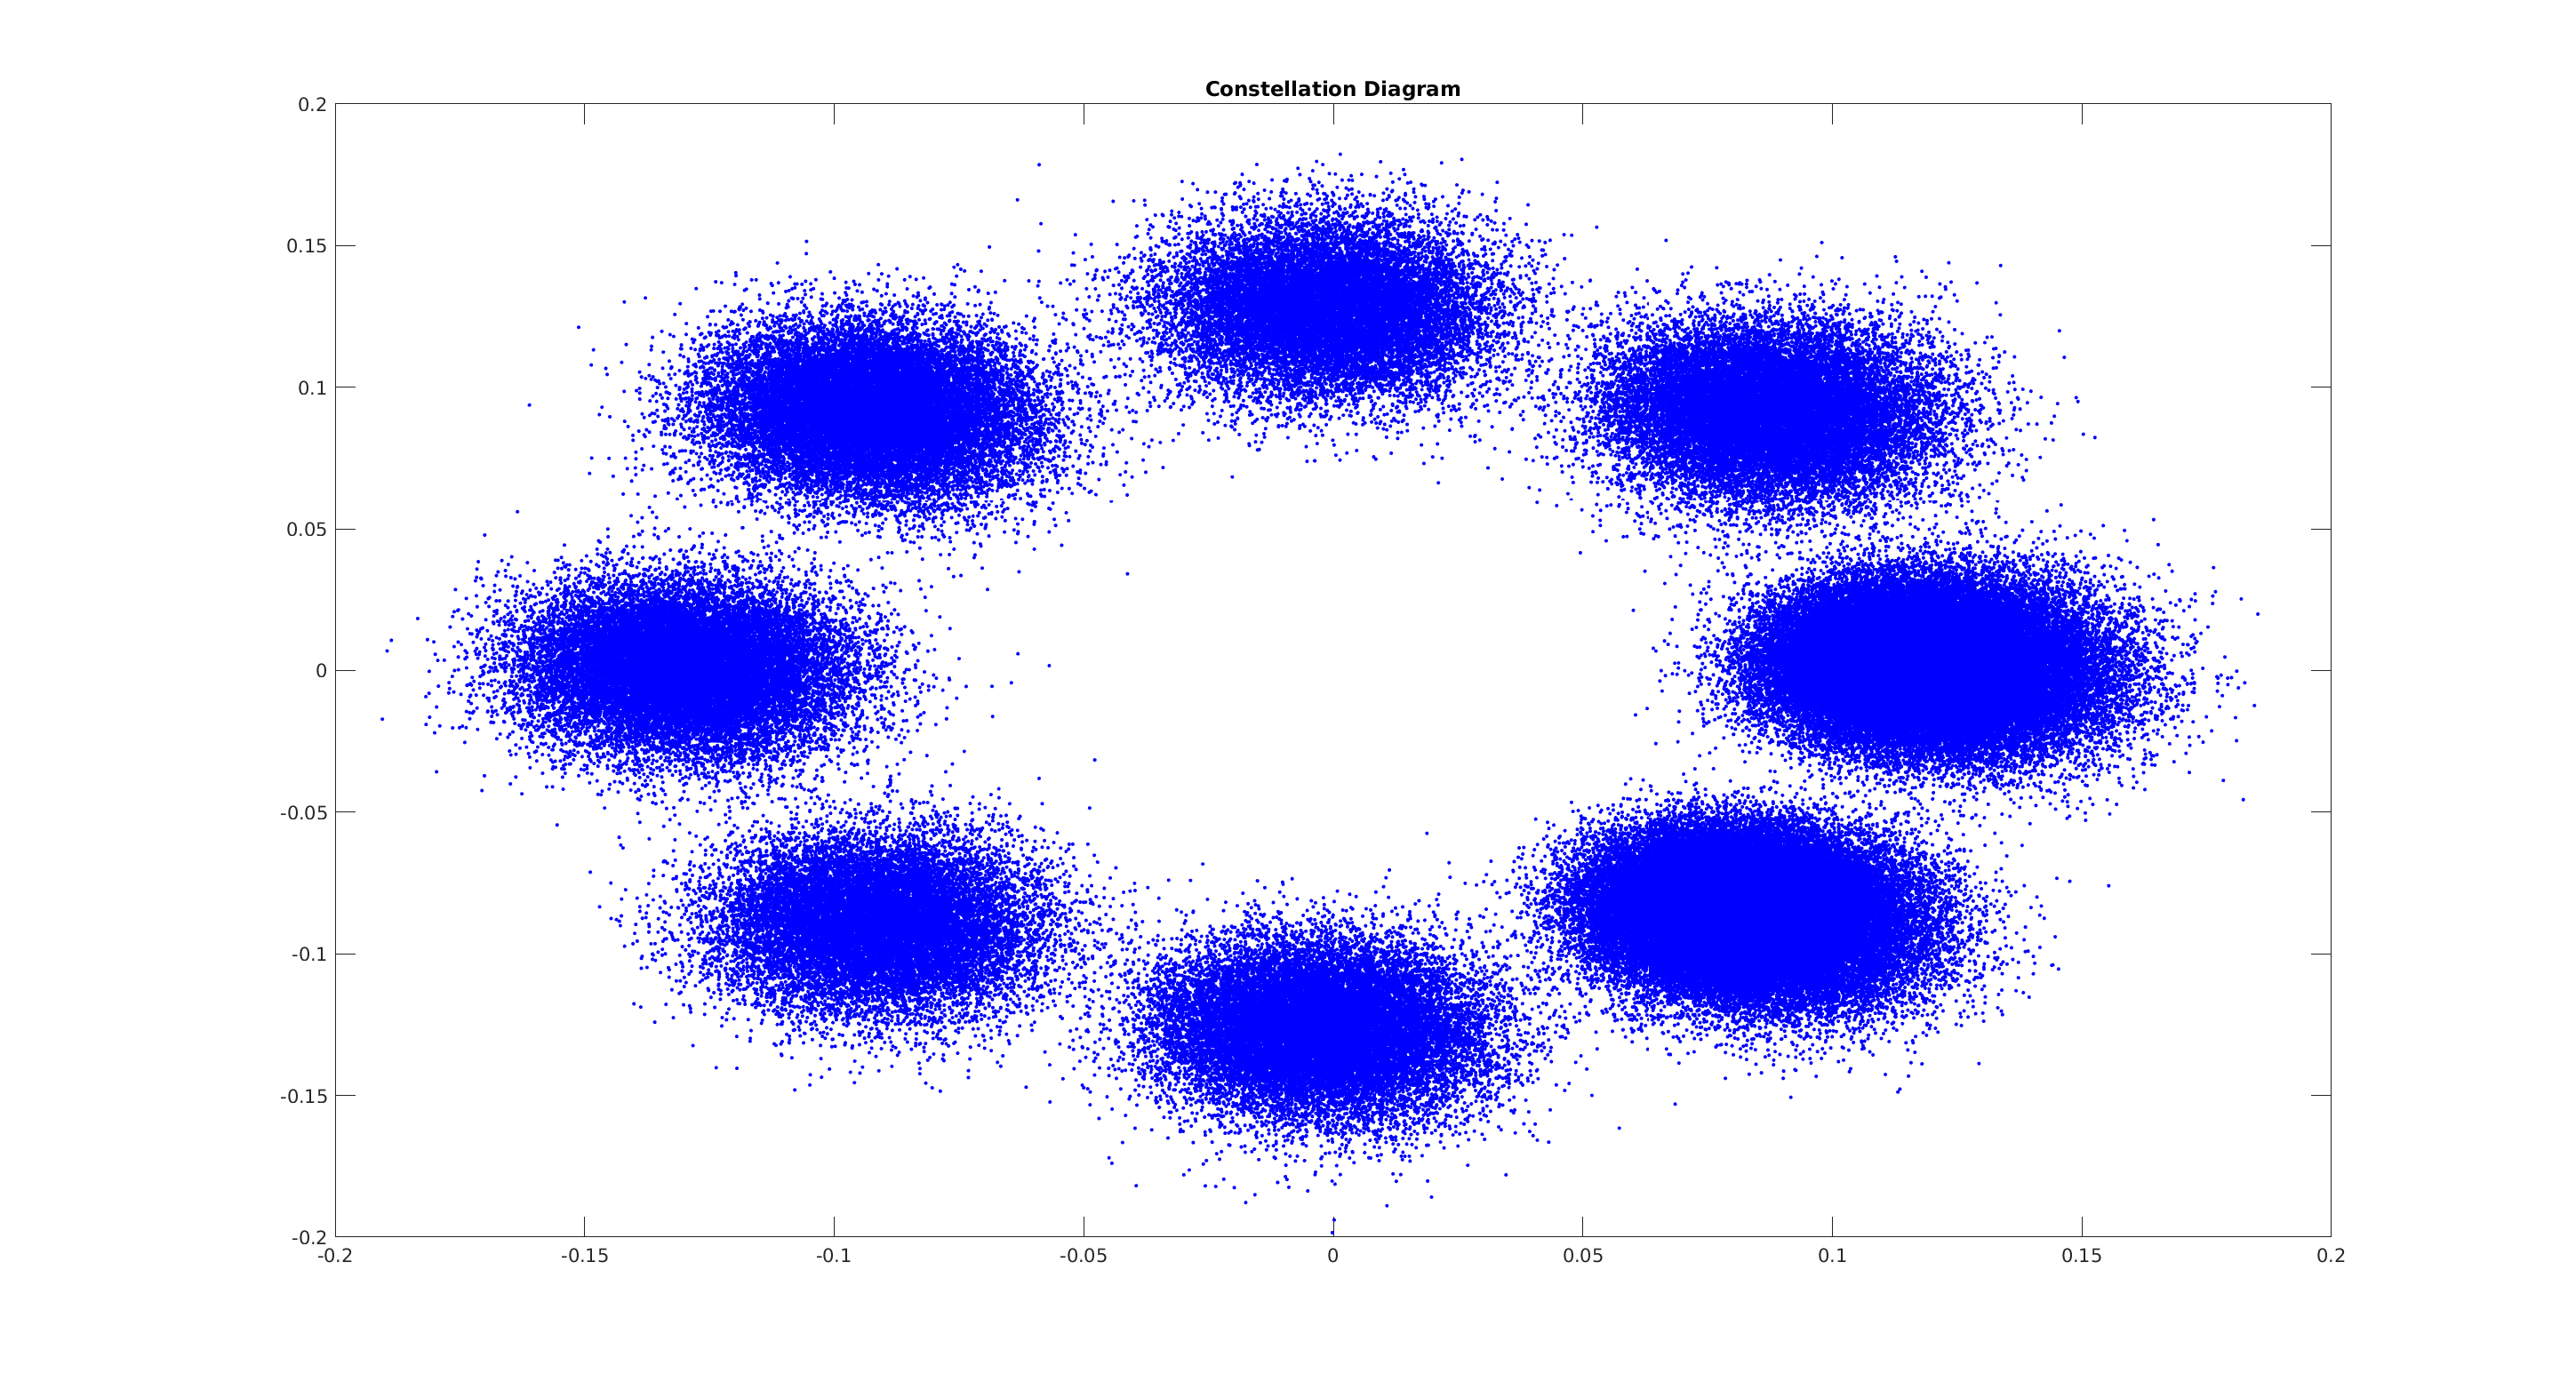
\includegraphics[width=0.9\columnwidth]{constellation15.png}
\caption{SNR=9dB}
\end{minipage}
\hfill
\begin{minipage}[t]{0.5\linewidth}
\centering
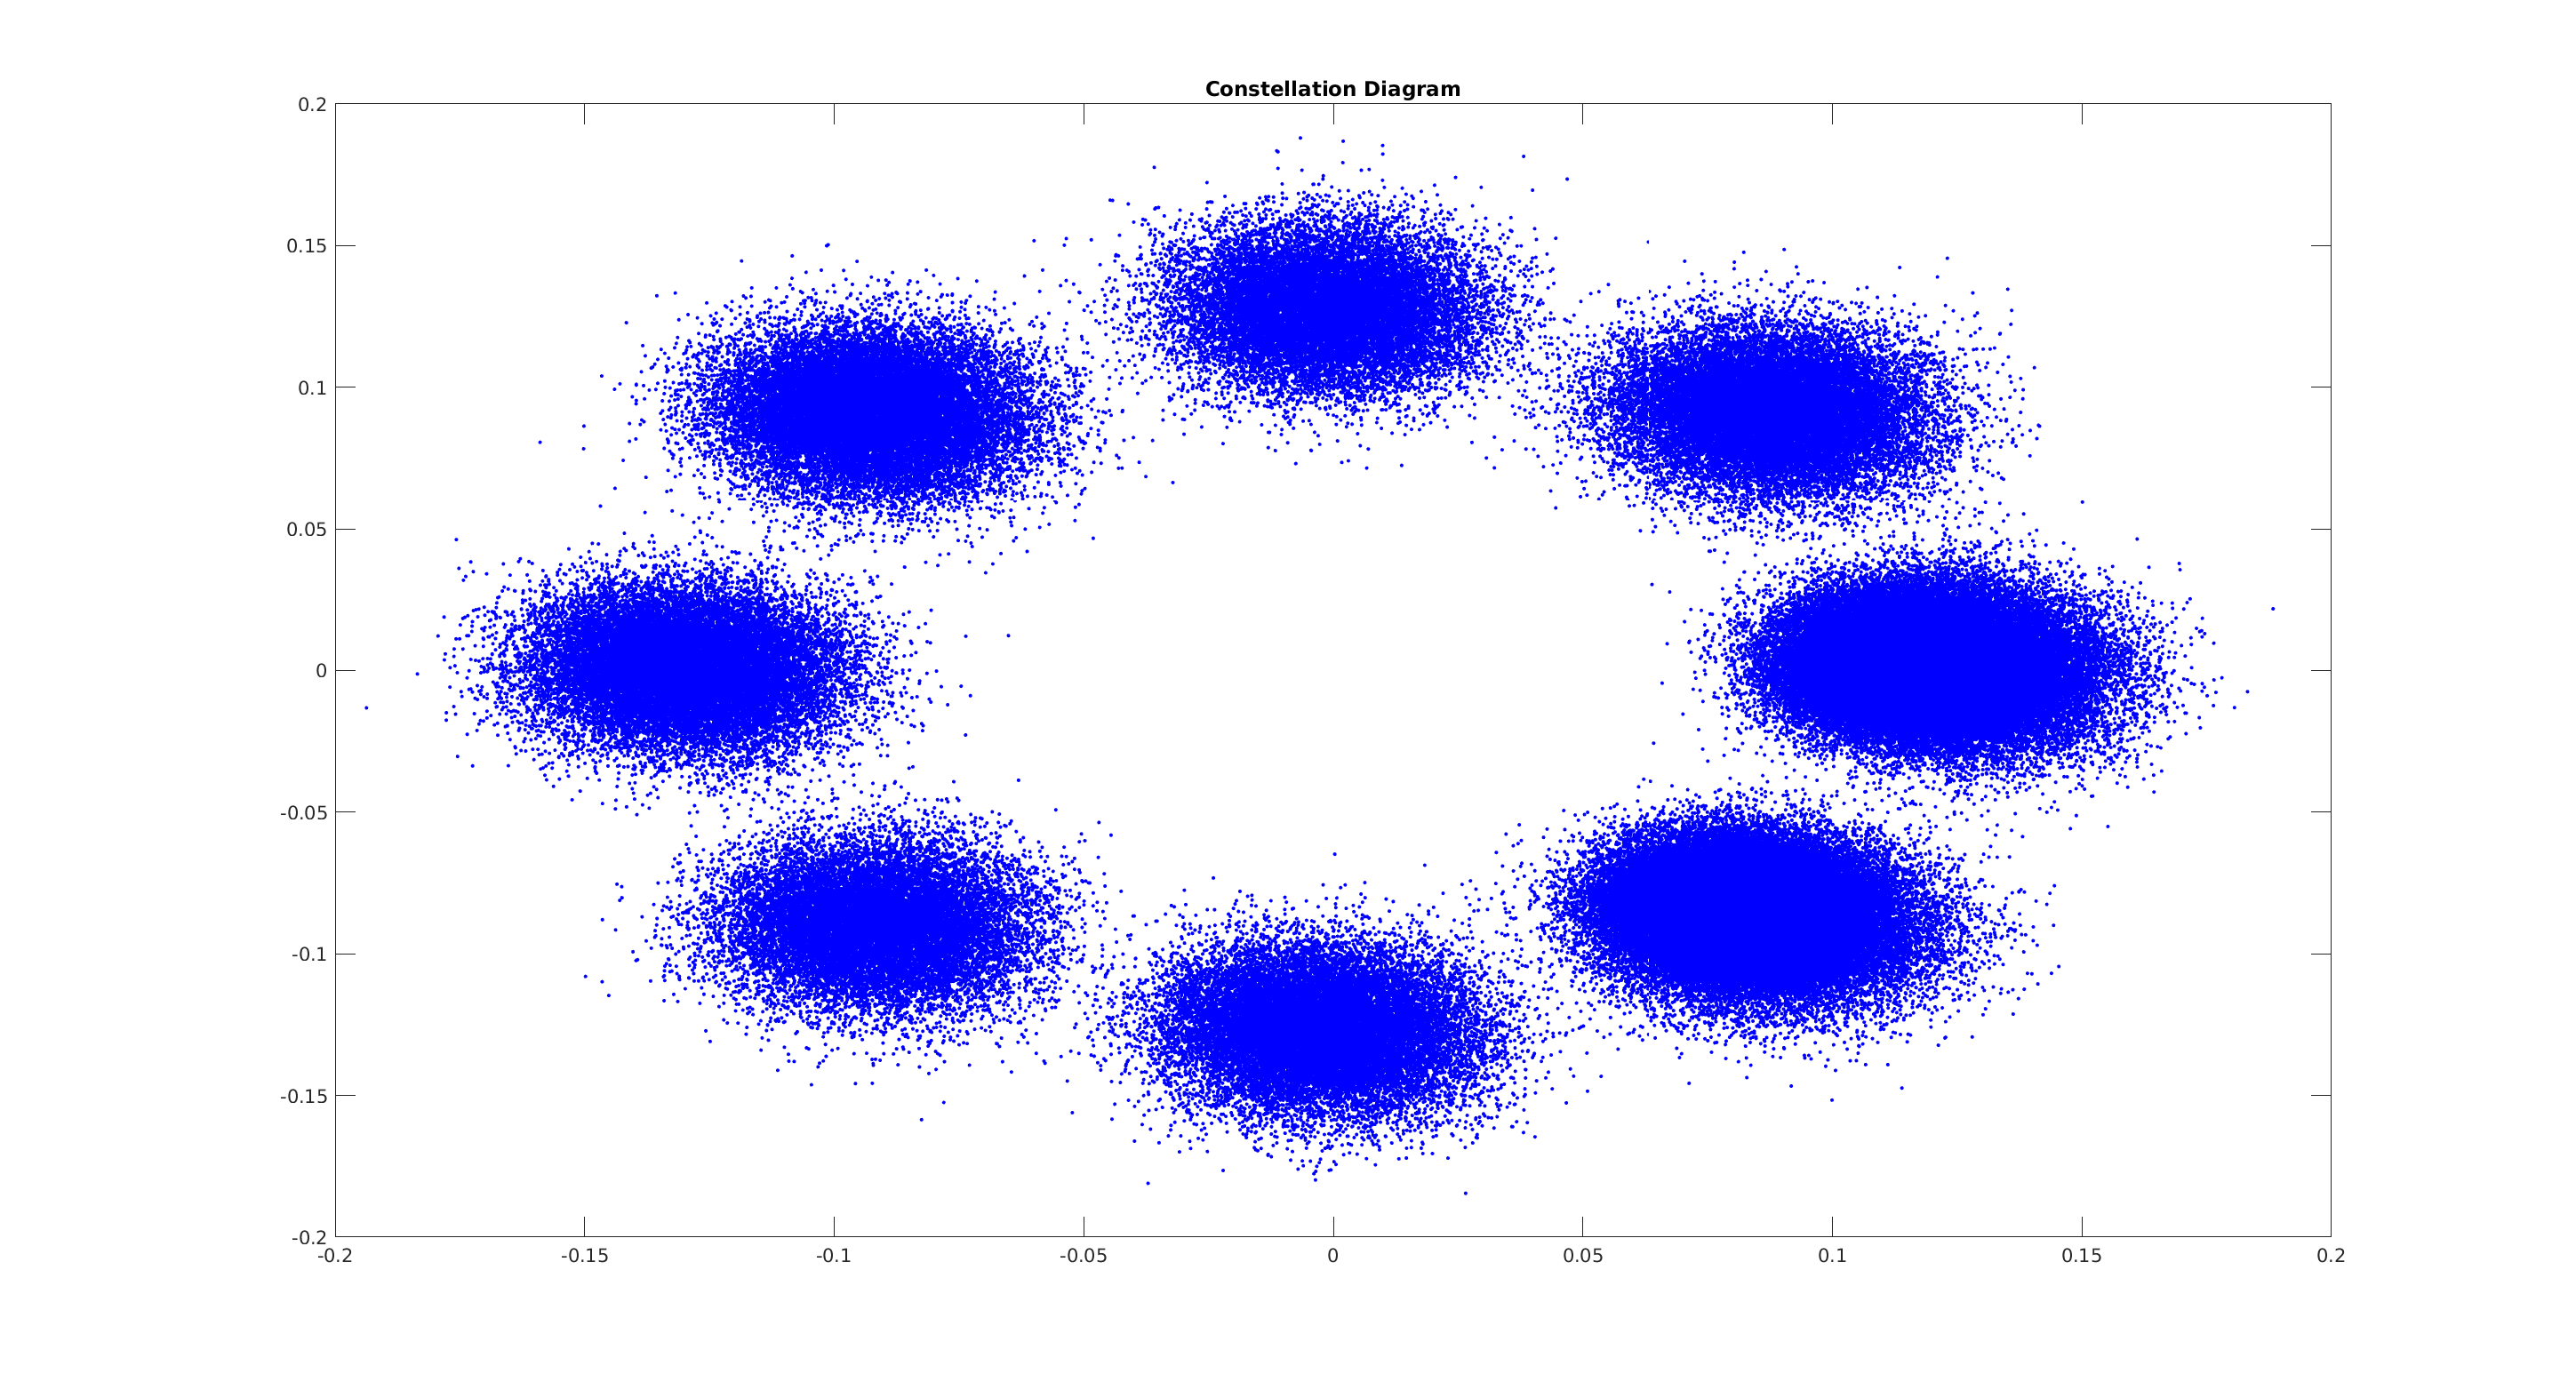
\includegraphics[width=0.9\columnwidth]{constellation16.png}
\caption{SNR=10dB}
\end{minipage}
\end{figure}

可以看到随着SNR的提升,星座图8个相位点逐渐清晰并彼此分离,表示此时判决的误码率不断下降。

\subsection{滤波器的影响}

使用等波纹方法设计的低通滤波器在EbN0较高时性能较差,与理想曲线相距较远,故尝试使用平方根升余弦滤波器,参数设置为凯泽窗,Beta=0.5,阶数为100阶,$F_s= 128000/3*8*2 \approx 682666 Hz, F_c = 128000/3 \approx 42666Hz$,参数设计、得到的星座图及最后的误码率曲线如下:

\begin{figure}[H]
\centering
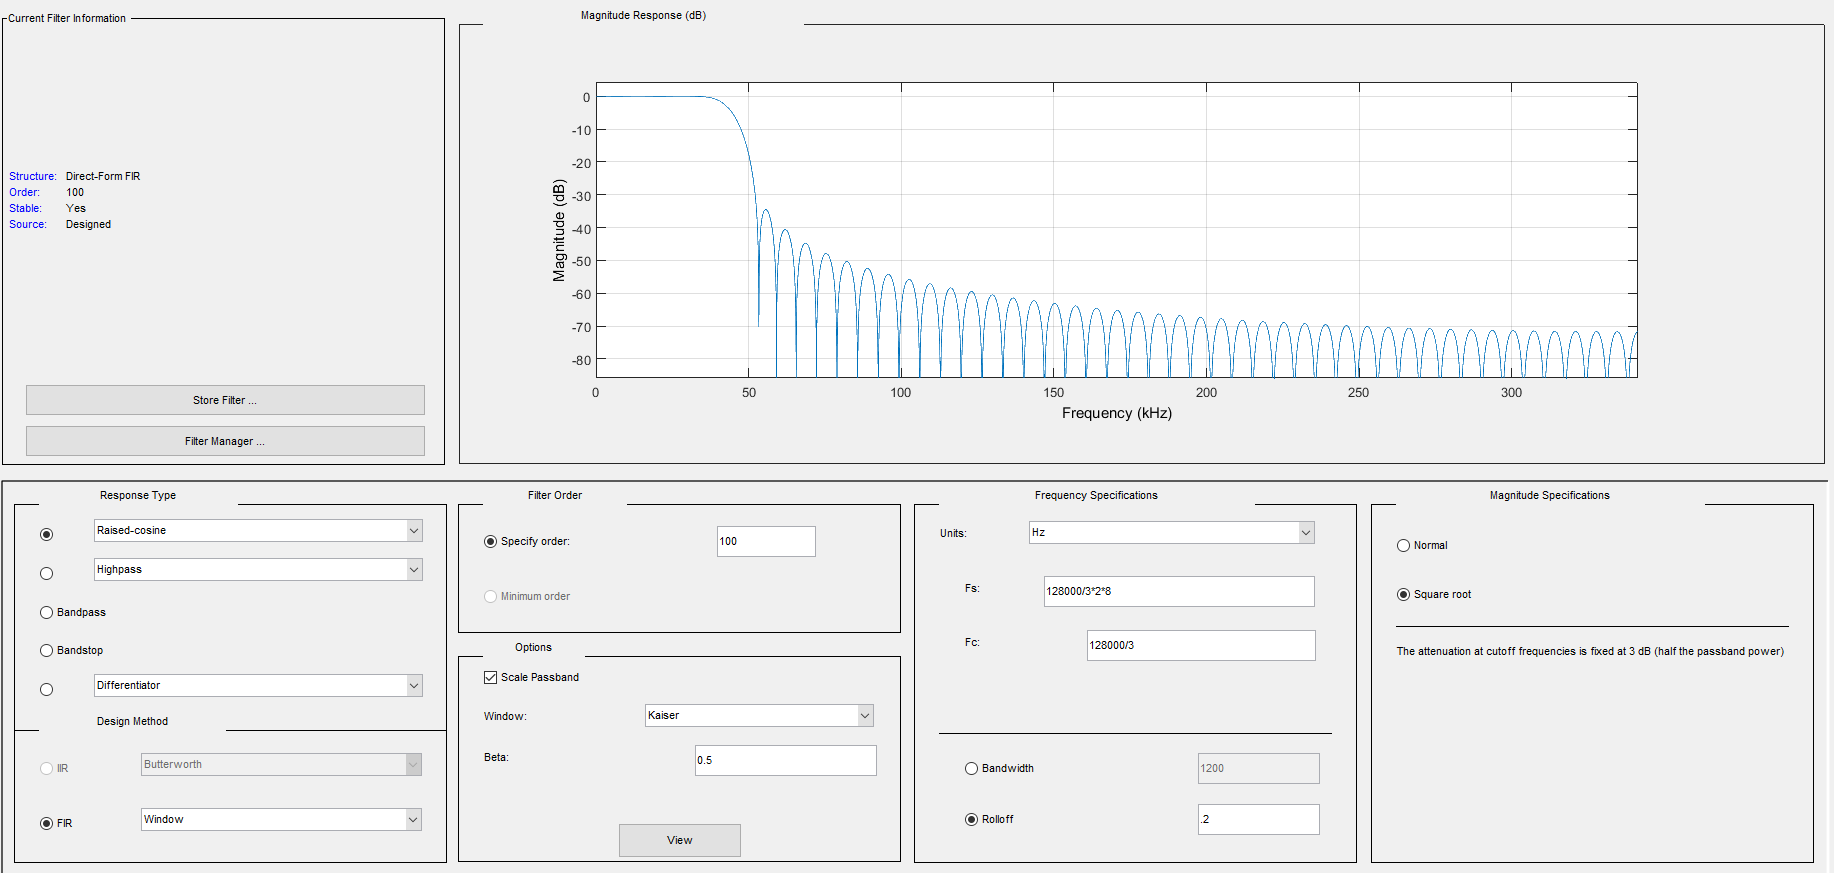
\includegraphics[width = \columnwidth]{srcparam.png}
\end{figure}

\begin{figure}[H]
\centering
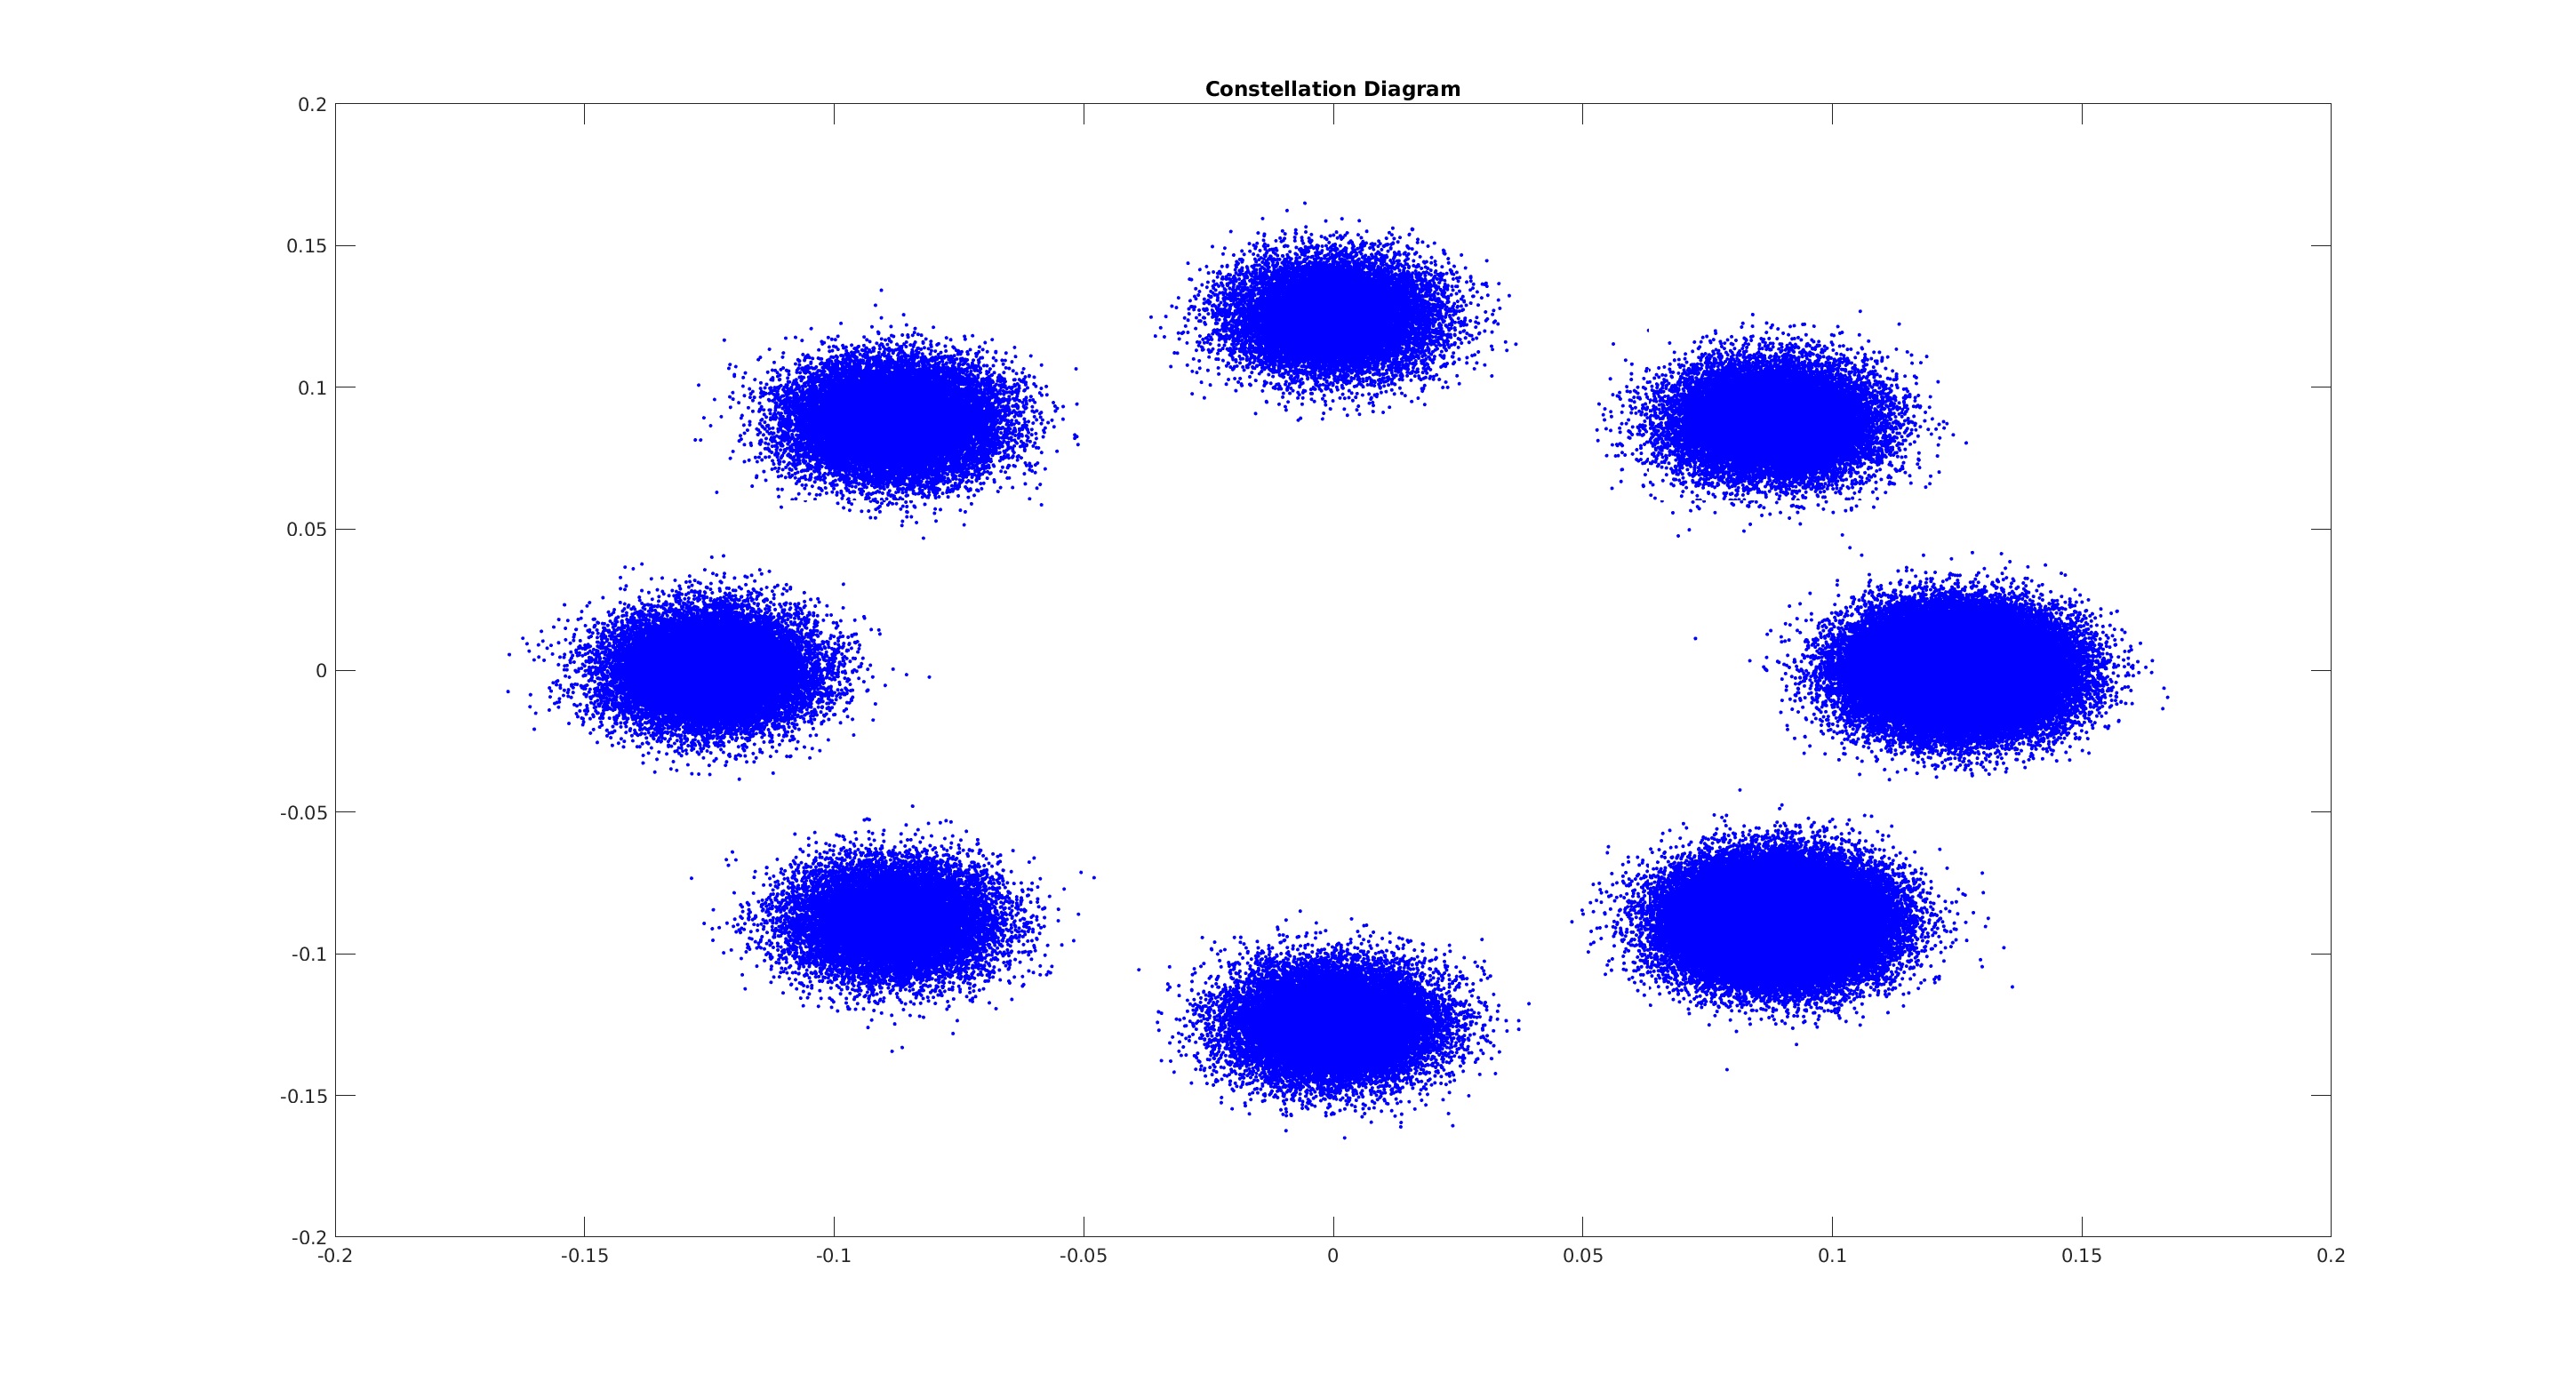
\includegraphics[width = \columnwidth]{constellation-src.png}
\end{figure}

\begin{figure}[H]
\centering
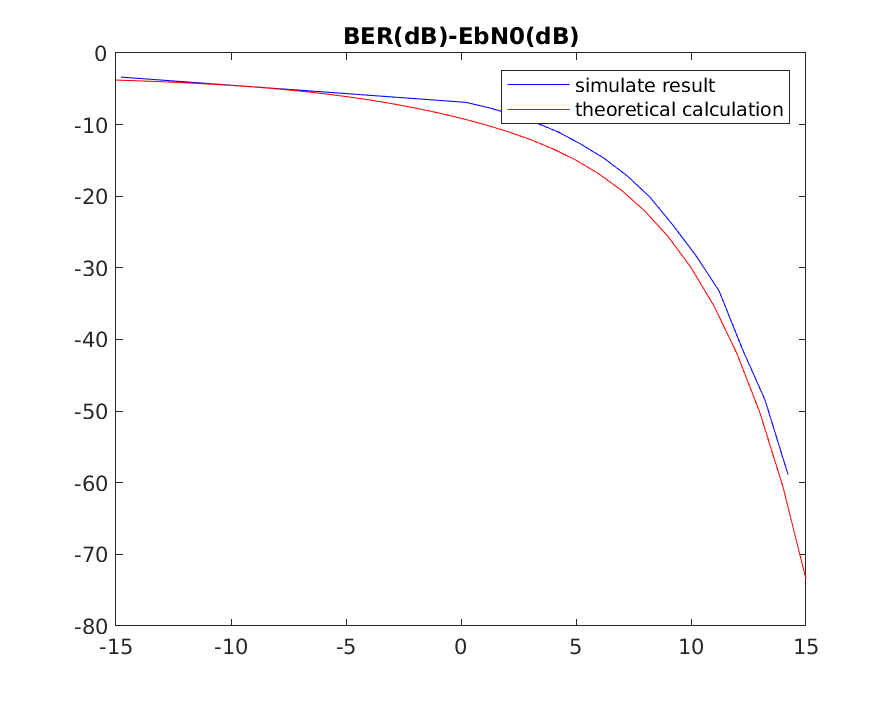
\includegraphics[width = \columnwidth]{BER-src.png}
\end{figure}

可以看到升余弦滤波器星座图得到的散点更集中于8个相位点附近,误码率与理想曲线吻合更好,说明平方根升余弦滤波器在解决符号间干扰的问题上性能突出。

\section{附0:辅助代码}

\subsection{dectobin.m}

实现十进制整数(包含正负)到二进制的转化。

\begin{lstlisting}
function bin = dectobin(dec, bit)
    bin = dec2bin(abs(dec), bit);
    for j = 1:length(dec)
        if dec(j,1) < 0
            for i = 1:bit
                if bin(j, i) == 48
                    bin(j, i) = 49;
                else
                    bin(j, i) = 48;
                end
            end
            bin(j, bit) = bin(j, bit) + 1;
            for i = bit:-1:2
                if bin(j, i) == 50
                    bin(j, i - 1) = bin(j, i - 1) + 1;
                    bin(j, i) = 48;
                end
            end
            if bin(j, 1) == 50
               bin(j, 1) = 48;
            end
        end
    end   
end
\end{lstlisting}

\subsection{HD.m}

自己设计的等波纹滤波器参数内容。

\begin{lstlisting}
function Hd = HD
%HD Returns a discrete-time filter object.

% MATLAB Code
% Generated by MATLAB(R) 9.4 and DSP System Toolbox 9.6.
% Generated on: 20-Jun-2018 00:42:54

% Equiripple Lowpass filter designed using the FIRPM function.

% All frequency values are in Hz.
Fs = 682666.66667;  % Sampling Frequency

Fpass = 42666.666667;    % Passband Frequency
Fstop = 46666.666667;    % Stopband Frequency
Dpass = 0.057501127785;  % Passband Ripple
Dstop = 0.0001;          % Stopband Attenuation
dens  = 20;              % Density Factor

% Calculate the order from the parameters using FIRPMORD.
[N, Fo, Ao, W] = firpmord([Fpass, Fstop]/(Fs/2), [1 0], [Dpass, Dstop]);

% Calculate the coefficients using the FIRPM function.
b  = firpm(N, Fo, Ao, W, {dens});
Hd = dfilt.dffir(b);

% [EOF]
\end{lstlisting}

\subsection{SRC.m}

自己设计的平方根升余弦滤波器参数内容。

\begin{lstlisting}
function Hd = SRC
%SRC Returns a discrete-time filter object.

% MATLAB Code
% Generated by MATLAB(R) 9.4 and DSP System Toolbox 9.6.
% Generated on: 19-Jun-2018 23:52:49

% FIR Window Raised-cosine filter designed using the FIRRCOS function.

% All frequency values are in Hz.
Fs = 682666.66667;  % Sampling Frequency

N    = 100;           % Order
Fc   = 42666.666667;  % Cutoff Frequency
TM   = 'Rolloff';     % Transition Mode
R    = 0.2;           % Rolloff
DT   = 'sqrt';        % Design Type
Beta = 0.5;           % Window Parameter

% Create the window vector for the design algorithm.
win = kaiser(N+1, Beta);

% Calculate the coefficients using the FIR1 function.
b  = firrcos(N, Fc/(Fs/2), R, 2, TM, DT, [], win);
Hd = dfilt.dffir(b);

% [EOF]
\end{lstlisting}

\subsection{ber\_standard.mat}

8PSK理想误码率曲线数据内容。


\end{spacing}
\end{document}